\documentclass[11pt,UTF8]{article}
\usepackage{ctex}
\usepackage{amsmath, amssymb, amsthm}
\usepackage{geometry}
\usepackage{enumerate}
\usepackage{bm}
\usepackage{graphicx}
\usepackage{ulem} % 提供 \sout 命令（删除线）
\usepackage[dvipsnames]{xcolor} % 提供更多颜色
\usepackage[colorlinks=true, % 启用彩色链接
linkcolor=black, % 内部链接颜色
urlcolor=blue, % 外部URL颜色
citecolor=ForestGreen, % 引用文献颜色
filecolor=magenta] % 本地文件链接颜色
{hyperref}

\geometry{left=2.5cm,right=2.5cm,top=2.5cm,bottom=2.5cm}

\title{离散数学 2026 春习题课笔记}
\author{讲师：刘易铖}
\date{\today}

\begin{document}

\maketitle

\tableofcontents


\section*{课前说明与作业反馈}

在正式开始习题讲解前，针对前几周的作业情况进行以下说明：
\begin{itemize}
    \item \textbf{教材版本：} 请务必核对教材版本，确保题目序号与要求一致。
    \item \textbf{解题规范：} 
    \begin{itemize}
        \item 判断题不能只给结论，必须写出详细理由（尤其是 PPT 上给出的思考题）。
        \item 证明题严禁“跳步”，应清晰呈现推导的前提条件和逻辑结论。
    \end{itemize}
    \item \textbf{提交要求：} 线上提交推荐使用 PDF 格式以便助教批改。若采用拍照方式，请确保字迹清晰、光线充足。
\end{itemize}

\newpage

\section{3月4日：集合、函数、序列与求和}

本节内容涵盖教材第 2.2 节（集合运算）、2.3 节（函数）及 2.4 节（序列与求和）。

\subsection{集合基本运算 (Section 2.2)}

在进行集合证明前，我们回顾两个基本概念：
\begin{enumerate}
    \item \textbf{子集定义：} $A \subseteq B \iff \forall x (x \in A \implies x \in B)$。
    \item \textbf{集合相等：} $A = B \iff A \subseteq B \land B \subseteq A$。
\end{enumerate}

\subsubsection*{习题 2.2-20}
\textbf{题目：} 设 $A, B, C$ 为集合，证明：
\begin{enumerate}[a)]
    \item $(A \cup B) \subseteq (A \cup B \cup C)$
    \item $(B - A) \cup (C - A) = (B \cup C) - A$
\end{enumerate}

\textbf{解答：}
\begin{itemize}
    \item \textbf{a) 的证明：}
    对于任意元素 $x \in A \cup B$，根据并集的定义可知 $x \in A$ 或 $x \in B$。
    显然，逻辑命题 $(x \in A \lor x \in B) \implies (x \in A \lor x \in B \lor x \in C)$ 恒成立。
    因此 $x \in A \cup B \cup C$。故 $(A \cup B) \subseteq (A \cup B \cup C)$ 得证。

    \item \textbf{e) 的证明：}
    我们需要从两个方向证明包含关系：
    \begin{enumerate}[1.]
        \item \textbf{证明 $(B - A) \cup (C - A) \subseteq (B \cup C) - A$：}
        设 $x \in (B - A) \cup (C - A)$，则 $x \in (B - A)$ 或 $x \in (C - A)$。
        若 $x \in (B - A)$，则 $x \in B$ 且 $x \notin A$；若 $x \in (C - A)$，则 $x \in C$ 且 $x \notin A$。
        在这两种情况下，都有 $x \notin A$ 且 ($x \in B$ 或 $x \in C$)。
        由并集定义得 $x \in (B \cup C)$，结合 $x \notin A$ 可知 $x \in (B \cup C) - A$。
        
        \item \textbf{证明 $(B \cup C) - A \subseteq (B - A) \cup (C - A)$：}
        设 $x \in (B \cup C) - A$，则 $x \in (B \cup C)$ 且 $x \notin A$。
        由 $x \in B \cup C$ 知 $x \in B$ 或 $x \in C$。
        若 $x \in B$，结合 $x \notin A$ 得 $x \in B - A$；
        若 $x \in C$，结合 $x \notin A$ 得 $x \in C - A$。
        因此 $x \in (B - A) \cup (C - A)$。
    \end{enumerate}
    综上所述，两集合相等。
\end{itemize}

\subsubsection*{习题 2.2-56}
\textbf{题目：} 求下列集合序列的并集 $\bigcup_{i=1}^{\infty} A_i$ 和交集 $\bigcap_{i=1}^{\infty} A_i$：
\begin{enumerate}[a)]
    \item $A_i = \{i, i + 1, i + 2, \dots \}$
    \item $A_i = \{0, i\}$
    \item $A_i = (0, i)$ （开区间）
    \item $A_i = (i, \infty)$ （开区间）
\end{enumerate}

\textbf{解答：}
\begin{itemize}
    \item \textbf{a)} $A_1=\{1,2,\dots\}, A_2=\{2,3,\dots\}$。并集为 $A_1 = \mathbb{Z}^+$；由于随着 $i$ 增大，集合不断变小且最小元素趋于无穷，交集为 $\emptyset$。
    \item \textbf{b)} 每个集合都包含 $0$，且 $A_i$ 包含正整数 $i$。并集为 $\{0\} \cup \mathbb{Z}^+$；交集为所有集合中共有的元素 $\{0\}$。
    \item \textbf{c)} $A_1=(0,1), A_2=(0,2)$。并集为取最大的范围 $(0, \infty)$；交集为取最小的范围 $(0, 1)$。
    \item \textbf{d)} $A_1=(1,\infty), A_2=(2,\infty)$。并集为 $A_1 = (1, \infty)$；交集为 $\emptyset$。
\end{itemize}

\subsection{函数性质 (Section 2.3)}

\subsubsection*{概念补充}
设 $f: A \to B$：
\begin{itemize}
    \item \textbf{单射 (Injective)：} $\forall a_1, a_2 \in A, f(a_1) = f(a_2) \implies a_1 = a_2$。
    \item \textbf{满射 (Surjective)：} $\forall b \in B, \exists a \in A, f(a) = b$。
    \item \textbf{双射 (Bijective)：} 既是单射又是满射。
\end{itemize}

\subsubsection*{习题 2.3-22}
\textbf{题目：} 判断下列函数是否为从实数集 $\mathbb{R}$ 到 $\mathbb{R}$ 的双射：
\begin{enumerate}[a)]
    \item $f(x) = -3x + 4$
    \item $f(x) = -3x^2 + 7$
    \item $f(x) = (x + 1)/(x + 2)$
    \item $f(x) = x^5 + 1$
\end{enumerate}

\textbf{解答提示：}
\begin{itemize}
    \item \textbf{b)} \textbf{不是双射}。因为它不是单射（如 $f(1) = f(-1) = 4$），且不是满射（值域为 $(-\infty, 7]$）。
    \item \textbf{c)} \textbf{不是从 $\mathbb{R}$ 到 $\mathbb{R}$ 的函数}。因为在 $x = -2$ 处无定义，定义域不满足全定义要求。
\end{itemize}

\subsubsection*{习题 2.3-76 (取整函数证明)}
\textbf{题目：} 证明或反驳下列关于下取整 $\lfloor x \rfloor$ 和上取整 $\lceil x \rceil$ 的命题：
\begin{enumerate}[a)]
    \item $\lfloor \lceil x \rceil \rfloor = \lceil x \rceil$
    \item $\lfloor x + y \rfloor = \lfloor x \rfloor + \lfloor y \rfloor$
    \item $\lceil \lceil x/2 \rceil / 2 \rceil = \lceil x/4 \rceil$
    \item $\lfloor \sqrt{\lceil x \rceil} \rfloor = \lfloor \sqrt{x} \rfloor$ 对于 $x > 0$
    \item $\lfloor x \rfloor + \lfloor y \rfloor + \lfloor x + y \rfloor \le \lfloor 2x \rfloor + \lfloor 2y \rfloor$
\end{enumerate}

\textbf{重点推导过程：}
\begin{itemize}
    \item \textbf{c) 的证明：}
    令 $n = \lceil x/2 \rceil \in \mathbb{Z}$。由定义知 $n-1 < x/2 \le n$，两边同除以 2 得 $\frac{n-1}{2} < \frac{x}{4} \le \frac{n}{2}$。
    \begin{itemize}
        \item 若 $n$ 是偶数，设 $n=2k$，则 $k-1/2 < x/4 \le k$，故 $\lceil x/4 \rceil = k = n/2 = \lceil n/2 \rceil$。
        \item 若 $n$ 是奇数，设 $n=2k+1$，则 $k < x/4 \le k+1/2$，故 $\lceil x/4 \rceil = k+1 = (n+1)/2 = \lceil n/2 \rceil$。
    \end{itemize}
    结论成立。

    \item \textbf{e) 的证明：}
    设 $x = m + \alpha, y = n + \beta$，其中 $m, n \in \mathbb{Z}, \alpha, \beta \in [0, 1)$。
    原不等式左边 $L = m + n + (m + n + \lfloor \alpha + \beta \rfloor) = 2m + 2n + \lfloor \alpha + \beta \rfloor$。
    右边 $R = (2m + \lfloor 2\alpha \rfloor) + (2n + \lfloor 2\beta \rfloor) = 2m + 2n + \lfloor 2\alpha \rfloor + \lfloor 2\beta \rfloor$。
    只需证 $\lfloor \alpha + \beta \rfloor \le \lfloor 2\alpha \rfloor + \lfloor 2\beta \rfloor$：
    \begin{itemize}
        \item 若 $\alpha + \beta < 1$，左边为 $0$，不等式显然成立。
        \item 若 $\alpha + \beta \ge 1$，则 $\alpha, \beta$ 中至少有一个 $\ge 1/2$（否则 $\alpha+\beta < 1$），故 $\lfloor 2\alpha \rfloor + \lfloor 2\beta \rfloor \ge 1$。左边为 $1$，不等式成立。
    \end{itemize}
\end{itemize}

\subsection{序列与递推关系 (Section 2.4)}

\subsubsection*{习题 2.4-16}
\textbf{题目：} 求解下列满足给定初始条件的递推关系：
\begin{enumerate}[a)]
    \item $a_n = 2a_{n-1} - 3, a_0 = -1$
    \item $a_n = -a_{n-1} + n - 1, a_0 = 7$
\end{enumerate}

\textbf{解答推导：}
\begin{itemize}
    \item \textbf{a) 的解法：}
    观察形式 $a_n - 3 = 2(a_{n-1} - 3)$。令 $b_n = a_n - 3$，则 $b_n = 2b_{n-1}$ 且 $b_0 = a_0 - 3 = -4$。
    这是一个等比数列，$b_n = -4 \cdot 2^n$。
    还原得 $a_n = -4 \cdot 2^n + 3 = 3 - 2^{n+2}$。

    \item \textbf{b) 的解法：}
    通过迭代发现：$a_n = -(-a_{n-2} + n - 2) + n - 1 = a_{n-2} + 1$。
    这说明序列每隔两项增加 1。
    计算首项：$a_0 = 7, a_1 = -7 + 1 - 1 = -7$。
    \begin{itemize}
        \item 当 $n$ 为偶数时，$a_n = a_0 + n/2 = 7 + n/2$。
        \item 当 $n$ 为奇数时，$a_n = a_1 + (n-1)/2 = -7 + (n-1)/2$。
    \end{itemize}
    合并公式为：$a_n = \frac{29(-1)^n + 2n - 1}{4}$。
\end{itemize}

\subsubsection*{思考题：幂和的闭式解}
\textbf{题目：} 求 $\sum_{k=1}^{n} k^4$ 的闭式表达式。
\textbf{思路：} 利用恒等式 $(k+1)^5 - k^5 = 5k^4 + 10k^3 + 10k^2 + 5k + 1$。
对 $k=1, \dots, n$ 求和，左侧发生消去（裂项），右侧代入已知的 $\sum k, \sum k^2, \sum k^3$ 公式，整理可得：
\[ \sum_{k=1}^{n} k^4 = \frac{n(n+1)(2n+1)(3n^2 + 3n - 1)}{30} \]



\section{3月11日：集合的基数与矩阵运算}

本节内容重点在于理解可数集（Countable Sets）的性质、集合势的比较，以及布尔矩阵的乘法。

\subsection{集合的基数 (Section 2.5)}

\subsubsection*{概念补充}
\begin{itemize}
    \item \textbf{可数集 (Countable Set)：} 如果一个集合是有限的，或者它与正整数集 $\mathbb{Z}^+$ 具有相同的基数（即存在双射），则称该集合为可数集。
    \item \textbf{势的比较：} $|A| \le |B|$ 当且仅当存在从 $A$ 到 $B$ 的单射函数。
    \item \textbf{Schröder-Bernstein 定理：} 若 $|A| \le |B|$ 且 $|B| \le |A|$，则 $|A| = |B|$（存在双射）。
\end{itemize}

\subsubsection*{习题 2.5-22}
\textbf{题目：} 假设 $A$ 是一个可数集。证明：如果存在一个从 $A$ 到 $B$ 的满射函数 $f$，那么 $B$ 也是可数的。

\textbf{解答思路与证明：}
\begin{enumerate}[1.]
    \item \textbf{前提分析：} 
    $A$ 是可数集，意味着 $|A| \le |\mathbb{Z}^+|$，即存在一个单射函数 $g: A \to \mathbb{Z}^+$。
    $f: A \to B$ 是满射，意味着对于 $B$ 中的每一个元素 $b$，在 $A$ 中至少有一个原像。

    \item \textbf{构造单射：} 
    为了证明 $B$ 可数，我们需要构造一个从 $B$ 到 $A$ 的单射函数 $f'$。
    对于每个 $b \in B$，定义 $f'(b) = a$，其中 $a$ 是原像集 $\{x \in A \mid f(x) = b\}$ 中编号最小的元素（利用 $A$ 可数这一性质给 $A$ 编号，或者基于选择公理）。
    由于 $f$ 是函数且每个 $b$ 至少有一个原像，这样构造的 $f': B \to A$ 满足：若 $b_1 \neq b_2$，则其原像集不相交，故 $f'(b_1) \neq f'(b_2)$。因此 $f'$ 是单射。

    \item \textbf{结论：} 
    由此可知 $|B| \le |A|$。由于 $|A| \le |\mathbb{Z}^+|$, 根据单射函数的复合性质，存在从 $B$ 到 $\mathbb{Z}^+$ 的单射 $g \circ f'$。
    所以 $|B| \le |\mathbb{Z}^+|$，即 $B$ 也是可数的。
\end{enumerate}

\subsubsection*{习题 2.5-24}
\textbf{题目：} 证明不存在无穷集合 $A$ 使得 $|A| < |\mathbb{Z}^+| = \aleph_0$。

\textbf{证明：}
根据定义，$\aleph_0$ 是最小的无穷势。
假设存在一个无穷集合 $A$。我们可以从 $A$ 中依次取出不同的元素 $a_1, a_2, a_3, \dots$。
由于 $A$ 是无穷的，这个过程可以永远进行下去，从而构造出一个 $A$ 的子集 $A' = \{a_1, a_2, \dots\}$，显然 $A'$ 是可数无穷的，即 $|A'| = \aleph_0$。
因为 $A' \subseteq A$，所以 $|A'| \le |A|$，即 $\aleph_0 \le |A|$。
这与假设 $|A| < \aleph_0$ 矛盾。因此，不存在势小于 $\aleph_0$ 的无穷集合。

\subsubsection*{习题 2.5-30}
\textbf{题目：} 证明所有系数为整数的二次方程 $ax^2 + bx + c = 0$ ($a \neq 0$) 的实数解组成的集合是可数的。

\textbf{解答：}
\begin{enumerate}[1.]
    \item \textbf{系数集合的可数性：}
    每个方程由三元组 $(a, b, c)$ 唯一确定，其中 $a, b, c \in \mathbb{Z}$ 且 $a \neq 0$。
    整数集 $\mathbb{Z}$ 是可数的，因此笛卡尔积 $\mathbb{Z}^3$ 也是可数的。令 $T = \{(a, b, c) \in \mathbb{Z}^3 \mid a \neq 0\}$，$T$ 作为可数集的子集，显然是可数的。
    
    \item \textbf{根集的可数性：}
    对于 $T$ 中的每一个元素 $t = (a, b, c)$，对应的二次方程最多有两个实数根。记其根集为 $R_t$，则 $|R_t| \le 2$。
    
    \item \textbf{并集性质：}
    所有此类方程的解集 $Q = \bigcup_{t \in T} R_t$。
    定理指出：\textbf{可数个可数集的并集仍然是可数的}。
    由于索引集 $T$ 可数，且每个 $R_t$ 是有限集（有限集必可数），因此 $Q$ 是可数的。
\end{enumerate}

\subsubsection*{思考题 (PPT-1)：比特串与无理数}
\textbf{题目：} 令 $\{0, 1\}^\omega$ 表示无限比特串集合，$\{0, 1\}^* 0^\omega$ 表示以无限个 $0$ 结尾的比特串集合。证明：
$|\{0, 1\}^\omega \setminus \{0, 1\}^* 0^\omega| = |\mathbb{I} \cap [0, 1]|$，其中 $\mathbb{I}$ 为无理数集。

\textbf{推导思路：}
\begin{enumerate}[1.]
    \item \textbf{左侧分析：} 无限比特串 $0.b_1b_2b_3\dots$ 对应区间 $[0, 1]$ 内实数的二进制表示。
    需要注意的是，某些实数有两套表示（如二进制的 $0.0111\dots = 0.1000\dots$）。
    集合 $\{0, 1\}^\omega \setminus \{0, 1\}^* 0^\omega$ 删除了所有以 $0$ 结尾的后缀（即删除了所有 $0.b_1\dots b_n 000\dots$ 形式的串）。
    这种做法实际上为每个二进制小数保留了唯一的表示（例如用 $0.0111\dots$ 代替 $0.1000\dots$），从而与半开区间 $(0, 1]$ 建立了一一对应。
    
    \item \textbf{右侧分析：} $\mathbb{I} \cap [0, 1]$ 是区间 $[0, 1]$ 除去所有有理数 $Q$。
    由于 $\mathbb{Q} \cap [0, 1]$ 是可数的，而 $[0, 1]$ 是不可数的，根据性质：若 $A$ 不可数且 $B$ 可数，则 $|A \setminus B| = |A|$。
    因此 $|\mathbb{I} \cap [0, 1]| = |[0, 1]|$。

    \item \textbf{结论：} 
    左侧集合与 $(0, 1]$ 等势，其势为 $c$（连续统势）；
    右侧集合与 $[0, 1]$ 等势，其势也为 $c$。故等式成立。
\end{enumerate}

\subsection{矩阵运算 (Section 2.6)}

\subsubsection*{概念补充：布尔乘积 (Boolean Product)}
设 $\mathbf{A}$ 是 $m \times k$ 矩阵，$\mathbf{B}$ 是 $k \times n$ 矩阵。其布尔乘积 $\mathbf{A} \odot \mathbf{B} = \mathbf{C}$ 的元素定义为：
\[ c_{ij} = (a_{i1} \land b_{1j}) \lor (a_{i2} \land b_{2j}) \lor \dots \lor (a_{ik} \land b_{kj}) \]
即在普通矩阵乘法的基础上，将乘法替换为逻辑与 ($\land$)，加法替换为逻辑或 ($\lor$)。

\subsubsection*{习题 2.6-28}
\textbf{题目：} 求 $\mathbf{A}$ 与 $\mathbf{B}$ 的布尔乘积，其中：
\[ \mathbf{A} = \begin{bmatrix} 1 & 0 & 0 & 1 \\ 0 & 1 & 0 & 1 \\ 1 & 1 & 1 & 1 \end{bmatrix}, \quad \mathbf{B} = \begin{bmatrix} 1 & 0 \\ 0 & 1 \\ 1 & 1 \\ 1 & 0 \end{bmatrix} \]

\textbf{解答：}
计算 $\mathbf{C} = \mathbf{A} \odot \mathbf{B}$：
\begin{itemize}
    \item $c_{11} = (1\land 1) \lor (0\land 0) \lor (0\land 1) \lor (1\land 1) = 1 \lor 0 \lor 0 \lor 1 = 1$
    \item $c_{12} = (1\land 0) \lor (0\land 1) \lor (0\land 1) \lor (1\land 0) = 0 \lor 0 \lor 0 \lor 0 = 0$
    \item 依次计算其他元素...
\end{itemize}
最终结果为：
\[ \mathbf{A} \odot \mathbf{B} = \begin{bmatrix} 1 & 0 \\ 1 & 1 \\ 1 & 1 \end{bmatrix} \]

\newpage

\section{3月16日：算法分析}

本节内容关注算法的设计与效率评估，重点在于二分查找的变体、排序算法的比较次数统计，以及贪心算法在找零问题中的适用性分析。

\subsection{二分查找的应用 (Problem ppt-1)}

\subsubsection*{概念补充：旋转有序数组}
一个严格递增有序数组 $a[1..n]$ 的旋转是指将数组的前 $k$ 个元素移到数组末尾。例如，$[1, 2, 3, 4, 5]$ 旋转后可能变为 $[3, 4, 5, 1, 2]$。

\subsubsection*{习题内容}
\textbf{题目：} 使用二分查找算法在一个经过旋转的有序数组中找到最小元素。

\textbf{算法步骤与思路：}
\begin{enumerate}[1.]
    \item \textbf{初始化：} 令左边界 $l = 1$，右边界 $r = n$。
    \item \textbf{循环条件：} 当 $l < r$ 时执行以下操作：
    \begin{itemize}
        \item 计算中间位置 $m = \lfloor(l + r) / 2\rfloor$。
        \item \textbf{判断分支 A：} 若 $a[m] \le a[r]$，说明从 $m$ 到 $r$ 段是递增的，最小值可能在 $m$ 处或其左侧。执行 $r := m$。
        \item \textbf{判断分支 B：} 否则（即 $a[m] > a[r]$），说明旋转点出现在 $m$ 的右侧，最小值必然在 $m+1$ 到 $r$ 之间。执行 $l := m + 1$。
    \end{itemize}
    \item \textbf{结束：} 循环结束时 $l = r$，此时 $a[l]$ 即为最小元素。
\end{enumerate}

\textbf{细节注意：}
\begin{itemize}
    \item \textbf{为何 $l$ 的更新是 $m+1$？} 若更新为 $l := m$，当 $l=3, r=4$ 时，$m=3$，若进入分支 B 则 $l$ 保持 3 不变，会导致程序陷入死循环。
    \item \textbf{区间含义：} 维护的区间 $[l, r]$ 始终保证包含最小值。
\end{itemize}

\subsection{排序算法的比较次数 (Problem ppt-2)}

\subsubsection*{习题内容}
\textbf{题目：} 对于降序序列 $n, n-1, \dots, 2, 1$，冒泡排序（Bubble Sort）和插入排序（Insertion Sort）分别需要多少次比较？

\textbf{解答与分析：}
\begin{enumerate}[1.]
    \item \textbf{冒泡排序：}
    根据伪代码，内层循环执行 $n-i$ 次比较。总比较次数为：
    \[ (n-1) + (n-2) + \dots + 1 = \frac{n(n-1)}{2} \]
    对于任何输入，标准冒泡排序的比较次数均为 $O(n^2)$。

    \item \textbf{插入排序：}
    当输入为倒序时，是插入排序的最坏情况。
    对于第 $j$ 个元素 $a_j$（从 $2$ 到 $n$），它需要与前面已排序的 $j-1$ 个元素逐一比较。
    在伪代码的 \texttt{while} 循环中，每次比较成功后都会执行 \texttt{insertPos := insertPos - 1}。
    对于降序序列，每次循环都需要比较 $j-1$ 次成功（移动）加上最后一次失败（判定边界），即 $j$ 次比较（或根据具体伪代码实现为 $2(i-1)+1$ 次判定）。
    最终计算总和得到比较次数为 $O(n^2)$ 级别。例如，对于序列 $[2, 1]$，插入排序需要 3 次判定/比较。
\end{enumerate}

\subsection{找零问题的贪心算法 (Problem ppt-3)}

\subsubsection*{习题内容}
\textbf{题目：} 针对第二套人民币纸币面额 $\{1, 2, 3, 5, 10\}$ 元，贪心算法 \texttt{change()} 是否总能产生张数最少的找零方案？

\textbf{解答：}
\textbf{结论：} 是的，对于该特定面额组合，贪心算法成立。

\textbf{证明逻辑分析：}
\begin{enumerate}[1.]
    \item \textbf{反例排除：} 贪心算法并不对所有面额组合有效。例如若面额为 $\{1, 8, 10\}$，找 24 元时：
    \begin{itemize}
        \item 贪心法：$10 \times 2 + 1 \times 4$（共 6 张）。
        \item 最优解：$8 \times 3$（共 3 张）。
    \end{itemize}
    
    \item \textbf{面额 $\{1, 2, 3, 5, 10\}$ 的特殊性证明：}
    我们需要证明在任何最优方案中，小面额纸币的张数是有上限的：
    \begin{itemize}
        \item 1元和2元：若有3张2元，可以用2张3元代替；若有2张1元，可以用1张2元代替。
        \item 3元：2张3元可以用1张5元和1张1元替换（张数不变但面值余量改变），更进一步，通过分类讨论发现小
        面额组合的总和若超过 10，总能被 10 元替换而减少张数。
    \end{itemize}
    通过计算，使用 $\{1, 2, 3, 5\}$ 能凑出的、且不满足替换条件的最高金额为 $1+2\times 2+3\times 3+5\times 1 = 19$（此为宽泛上限）。实际上，经过更细致的范围缩减，可以证明当总金额 $\ge 10$ 时，使用 10 元纸币必然是最优选择的一部分。
\end{enumerate}



\section{3月18日：函数的增长与算法复杂度}

本节内容重点在于使用大 $O$ 记号（Big-$O$ notation）评估函数的增长率，并分析具体算法的时间复杂度。

\subsection{函数的增长 (Section 3.2)}

\subsubsection*{概念补充}
\begin{itemize}
    \item \textbf{大 $O$ 记号定义：} 设 $f$ 和 $g$ 是从整数集或实数集到实数集的函数。如果存在常数 $C$ 和 $k$，使得当 $x > k$ 时，$|f(x)| \le C|g(x)|$，则称 $f(x)$ 是 $O(g(x))$。
    \item \textbf{增长阶级参考：} $1 < \log n < n < n \log n < n^2 < 2^n < n! < n^n$。
\end{itemize}

\subsubsection*{习题 3.2-26}
\textbf{题目：} 给出下列每个函数的渐进大 $O$ 估计：
\begin{enumerate}[a)]
    \item $f(n) = (n^3 + n^2 \log n)(\log n + 1) + (17 \log n + 19)(n^3 + 2)$
    \item $f(n) = (2^n + n^2)(n^3 + 3^n)$
    \item $f(n) = (n^n + n 2^n + 5^n)(n! + 5^n)$
\end{enumerate}

\textbf{解答提示：} 在处理乘积和求和的大 $O$ 估计时，只需保留增长最快的项。
\begin{itemize}
    \item \textbf{a) 的分析：}
    第一部分 $(n^3 + n^2 \log n)(\log n + 1) \approx n^3 \cdot \log n = O(n^3 \log n)$。
    第二部分 $(17 \log n + 19)(n^3 + 2) \approx \log n \cdot n^3 = O(n^3 \log n)$。
    故整体为 $O(n^3 \log n)$。
    
    \item \textbf{b) 的分析：}
    第一括号中 $2^n$ 增长最快，第二括号中 $3^n$ 增长最快。
    故 $f(n) = O(2^n \cdot 3^n) = O(6^n)$。
    
    \item \textbf{c) 的分析：}
    第一括号中 $n^n$ 占据主导，第二括号中 $n!$ 增长远快于 $5^n$。
    故 $f(n) = O(n^n \cdot n!)$。
\end{itemize}

\subsubsection*{习题 3.2-42 (关键证明题)}
\textbf{题目：} 假设 $f(x)$ 是 $O(g(x))$。是否可以推出 $2^{f(x)}$ 也是 $O(2^{g(x)})$？

\textbf{解答：}
\textbf{结论：} 不可以（不成立）。
\textbf{证明（反例法）：}
取 $f(x) = 2x$ 且 $g(x) = x$。
显然，由于 $2x \le 2 \cdot x$ 对于所有 $x > 0$ 成立，所以 $f(x)$ 是 $O(g(x))$。
然而，考虑它们的指数形式：
$2^{f(x)} = 2^{2x} = 4^x$，而 $2^{g(x)} = 2^x$。
计算它们的比值：$\frac{4^x}{2^x} = 2^x$。
当 $x \to \infty$ 时，$2^x \to \infty$，不存在常数 $C$ 使得 $4^x \le C \cdot 2^x$ 始终成立。
因此，$2^{f(x)}$ 不是 $O(2^{g(x)})$。

\subsection{算法复杂度 (Section 3.3)}

\subsubsection*{习题 3.3-12}
\textbf{题目：} 证明矩阵求最小值算法（Matrix-minimum algorithm）的时间复杂度为 $\Theta(n^3)$。

\textbf{证明过程：}
该算法通常涉及三重嵌套循环。设 $T(n)$ 为比较总次数：
\[ T(n) = \sum_{i=1}^{n} \sum_{j=i+1}^{n} \sum_{k=i+1}^{j} 1 = \sum_{i=1}^{n} \sum_{j=i+1}^{n} (j - i) \]
\begin{enumerate}[1.]
    \item \textbf{上界证明 ($O(n^3)$)：}
    三重循环的每一层规模都不会超过 $n$，因此总次数显然满足 $T(n) \le n \cdot n \cdot n = O(n^3)$。
    
    \item \textbf{下界证明 ($\Omega(n^3)$)：}
    为了证明下界，我们缩小索引范围。考虑 $i \le n/4$ 且 $j \ge 3n/4$ 的情况：
    在这种情况下，满足条件的 $(i, j)$ 对数大约有 $(n/4) \cdot (n/4) = n^2/16$ 对。
    对于每一对这样的 $(i, j)$，由于 $j - i \ge 3n/4 - n/4 = n/2$，
    其最内层循环的累加贡献至少为 $n/2$。
    则总和 $T(n) \ge (n/4) \cdot (n/4) \cdot (n/2) = n^3/32 = \Omega(n^3)$。
\end{enumerate}
由于 $T(n)$ 既是 $O(n^3)$ 又是 $\Omega(n^3)$，故 $T(n) = \Theta(n^3)$。

\subsubsection*{习题 3.3-13 \& 14}
\textbf{题目：} 
13. 给出计算多项式 $P(x) = a_nx^n + a_{n-1}x^{n-1} + \dots + a_1x + a_0$ 在 $x=c$ 处取值的传统算法。
14. 是否存在更高效的算法？

\textbf{解答说明：}
\begin{itemize}
    \item \textbf{传统算法：} 逐项计算 $x^i$ 再乘系数，复杂度为 $O(n^2)$。
    \item \textbf{高效算法（秦九韶算法/Horner's Method）：}
    通过嵌套重写多项式：$P(x) = (\dots((a_nx + a_{n-1})x + a_{n-2})x + \dots + a_1)x + a_0$。
    该算法仅需 $n$ 次乘法和 $n$ 次加法，时间复杂度优化至 $O(n)$。
\end{itemize}



\section{3月25日：数学归纳法与强归纳法}

本节内容重点在于掌握归纳法的证明规范，理解强归纳法与标准归纳法的区别，并探讨归纳假设的加强技巧。

\subsection{数学归纳法 (Section 5.1)}

\subsubsection*{概念补充：数学归纳法的步骤}
证明命题 $P(n)$ 对所有正整数 $n \ge n_0$ 成立：
\begin{enumerate}
    \item \textbf{基础步 (Basis Step)：} 证明 $P(n_0)$ 成立。
    \item \textbf{归纳步 (Inductive Step)：} 证明“若 $P(k)$ 成立，则 $P(k+1)$ 也成立”。其中 $P(k)$ 称为归纳假设 (Inductive Hypothesis)。
\end{enumerate}

\subsubsection*{习题 5.1-19}
\textbf{题目：} 证明对于所有大于 $1$ 的整数 $n$，下式恒成立：
\[ 1 + \frac{1}{4} + \frac{1}{9} + \dots + \frac{1}{n^2} < 2 - \frac{1}{n} \]

\textbf{证明过程：}
\begin{enumerate}[1.]
    \item \textbf{基础步：} 当 $n=2$ 时，左边 $= 1 + \frac{1}{4} = 1.25$；右边 $= 2 - \frac{1}{2} = 1.5$。由于 $1.25 < 1.5$，故 $P(2)$ 成立。
    \item \textbf{归纳步：} 假设 $P(k)$ 成立，即 $\sum_{j=1}^{k} \frac{1}{j^2} < 2 - \frac{1}{k}$。
    我们需要证 $P(k+1)$ 成立，即 $\sum_{j=1}^{k+1} \frac{1}{j^2} < 2 - \frac{1}{k+1}$。
    由归纳假设得：
    \[ \sum_{j=1}^{k+1} \frac{1}{j^2} = \sum_{j=1}^{k} \frac{1}{j^2} + \frac{1}{(k+1)^2} < 2 - \frac{1}{k} + \frac{1}{(k+1)^2} \]
    只需证 $2 - \frac{1}{k} + \frac{1}{(k+1)^2} \le 2 - \frac{1}{k+1}$，等价于证明：
    \[ \frac{1}{(k+1)^2} \le \frac{1}{k} - \frac{1}{k+1} = \frac{(k+1)-k}{k(k+1)} = \frac{1}{k(k+1)} \]
    由于 $k(k+1) < (k+1)^2$ 对 $k \ge 2$ 显然成立，故分式不等式成立。
\end{enumerate}
结论：原命题对所有 $n > 1$ 成立。

\subsubsection*{习题 5.1-74 (关于归纳假设的加强)}
\textbf{题目：} 说明为什么不能直接用归纳法证明 $\sum_{j=1}^{n} \frac{1}{j^2} < 2$，并解释该命题与习题 19 的关系。

\textbf{分析：}
如果我们直接设归纳假设为 $\sum_{j=1}^{k} \frac{1}{j^2} < 2$，在归纳步中：
$\sum_{j=1}^{k+1} \frac{1}{j^2} = (\sum_{j=1}^{k} \frac{1}{j^2}) + \frac{1}{(k+1)^2} < 2 + \frac{1}{(k+1)^2}$。
由于 $2 +$ 一个正数必然大于 $2$，我们无法推导出结果仍然小于 $2$。
\textbf{启示：} 归纳证明中有时需要一个“更强”的命题（如习题 19 中减去 $1/n$）作为中介，才能使归纳步顺利闭合。

\subsection{强归纳法 (Section 5.2)}

\subsubsection*{概念补充：强归纳法 (Strong Induction)}
在归纳步中，假设 $P(n_0), P(n_0+1), \dots, P(k)$ 全部成立，以此推导 $P(k+1)$。

\subsubsection*{习题 5.2-6 (邮票问题)}
\textbf{题目：} 
a) 确定仅用 3 分和 10 分邮票可以凑出的邮资额。
b) 用数学归纳法证明结论。
c) 用强归纳法证明结论。

\textbf{解答与证明：}
\textbf{a) 结论：} 可以凑出的额度为 3, 6, 9, 10, 12, 13, 15, 16 以及所有 $\ge 18$ 的整数。

\textbf{b) 数学归纳法 (k $\to$ k+1)：}
基础步 $P(18)$ 成立 ($3\times 6$)。
归纳步：假设 $P(k)$ 成立 ($k \ge 18$)。
\begin{itemize}
    \item 若凑出 $k$ 的方案中包含两张 10 分，将其换成七张 3 分，总额增 1。
    \item 若方案中 10 分邮票少于两张，由于 $k \ge 18$，则 3 分邮票至少有六张。将三张 3 分换成一张 10 分，总额增 1。
\end{itemize}

\textbf{c) 强归纳法：}
基础步：验证 $P(18), P(19), P(20)$ 均成立。
归纳步：假设对于 $18 \le j \le k$ 的 $P(j)$ 均成立 ($k \ge 20$)。
考虑凑出 $k+1$ 的方案：因为 $P(k-2)$ 成立，只需在其方案基础上增加一张 3 分邮票即可得到 $k+1$。

\subsubsection*{习题 5.2-10 (巧克力问题)}
\textbf{题目：} 将一块含有 $n$ 个小方块的巧克力折断成 $n$ 个独立的单块，需要折断多少次？

\textbf{解答：} 
\textbf{结论：} 恰好需要 $n-1$ 次。
\textbf{强归纳证明：}
基础步：$n=1$ 时，无需折断，次数为 $0 = 1-1$，成立。
归纳假设：对于所有 $1 \le m \le k$，分割 $m$ 块巧克力需 $m-1$ 次。
证明 $P(k+1)$：第一次折断会将巧克力分成大小为 $a$ 和 $b$ 的两块，其中 $a+b = k+1$ 且 $a,b \ge 1$。
根据假设，分割这两块分别需要 $a-1$ 次和 $b-1$ 次。
总次数 $= 1 + (a-1) + (b-1) = a+b-1 = (k+1)-1$。
结论得证。

\subsubsection*{习题 5.2-34 (复杂求和式证明)}
\textbf{题目：} 证明 $\sum_{j=1}^{n} j(j+1)\dots(j+k-1) = \frac{n(n+1)\dots(n+k)}{k+1}$ 对所有正整数 $n, k$ 成立。

\textbf{解答提示：} 对 $n$ 做归纳（将 $k$ 视为参数）。
基础步 ($n=1$)：左边 $= 1\cdot 2\dots k = k!$；右边 $= \frac{1\cdot 2\dots(k+1)}{k+1} = k!$。
归纳步：假设 $n$ 时成立。对于 $n+1$：
\[ \text{左边} = \sum_{j=1}^{n} (\dots) + (n+1)(n+2)\dots(n+k) \]
代入假设后提取公因子 $(n+1)\dots(n+k)$，括号内剩下 $\frac{n}{k+1} + 1 = \frac{n+k+1}{k+1}$。
整理即得 $\frac{(n+1)(n+2)\dots(n+k+1)}{k+1}$。



\section{第5.3节：递归定义与结构归纳法}

本节重点在于掌握递归定义（Recursive Definition）集合或结构的方法，以及与之配套的\textbf{结构归纳法}（Structural Induction）证明技巧。结构归纳法是普通数学归纳法在递归定义对象上的自然推广。

\subsection{递归定义与结构归纳法 (Section 5.3)}

\subsubsection*{概念补充}
\begin{itemize}
    \item \textbf{递归定义：} 对集合 $S$ 的递归定义通常包含两部分——\textbf{基础步骤}（指定最原始的元素）和\textbf{递归步骤}（给出从已有元素构造新元素的规则）。隐含地，只有经有限次应用上述规则得到的元素才属于 $S$。
    \item \textbf{结构归纳法：} 要证明递归定义集合中\textbf{所有}元素都满足某性质 $P$，只需验证：
    \begin{enumerate}[1.]
        \item \textbf{基础步：} 所有由基础步骤直接给出的元素满足 $P$；
        \item \textbf{归纳步：} 若已有元素满足 $P$，则通过递归规则生成的新元素也满足 $P$。
    \end{enumerate}
    \item \textbf{字符串递归定义：} 字母表 $\Sigma$ 上的字符串集合 $\Sigma^*$ 可递归定义为基础步 $\lambda \in \Sigma^*$（空串），递归步：若 $w \in \Sigma^*$ 且 $x \in \Sigma$，则 $wx \in \Sigma^*$。字符串的反转（Reversal）递归定义为：$\lambda^R = \lambda$；$(wx)^R = x w^R$。
\end{itemize}

\subsubsection*{习题 5.3-14}
\textbf{题目：} 证明当 $n$ 是正整数时，$f_{n+1}f_{n-1} - f_n^2 = (-1)^n$，其中 $f_n$ 为第 $n$ 个斐波那契数（规定 $f_0=0, f_1=1, f_2=1$）。

\textbf{证明：} 对正整数 $n$ 使用数学归纳法。

\begin{enumerate}[1.]
    \item \textbf{基础步：} 当 $n=1$ 时，
    \[ f_2 f_0 - f_1^2 = 1 \cdot 0 - 1^2 = -1 = (-1)^1 \]
    等式成立。

    \item \textbf{归纳步：} 假设当 $n=k$（$k \ge 1$）时等式成立，即
    \[ f_{k+1}f_{k-1} - f_k^2 = (-1)^k \tag{IH} \]
    需证 $n=k+1$ 时，$f_{k+2}f_k - f_{k+1}^2 = (-1)^{k+1}$。

    由斐波那契递推关系 $f_{k+2} = f_{k+1} + f_k$，左边可展开为：
    \begin{align*}
        f_{k+2}f_k - f_{k+1}^2
        &= (f_{k+1} + f_k)f_k - f_{k+1}^2 \\
        &= f_{k+1}f_k + f_k^2 - f_{k+1}^2
    \end{align*}
    由归纳假设 (IH) 可知 $f_k^2 = f_{k+1}f_{k-1} - (-1)^k$，代入上式：
    \begin{align*}
        &= f_{k+1}f_k + \bigl[f_{k+1}f_{k-1} - (-1)^k\bigr] - f_{k+1}^2 \\
        &= f_{k+1}(f_k + f_{k-1} - f_{k+1}) + (-1)^{k+1}
    \end{align*}
    由于 $f_k + f_{k-1} = f_{k+1}$，括号内为 $0$，于是：
    \[ f_{k+2}f_k - f_{k+1}^2 = (-1)^{k+1} \]
    归纳步成立。
\end{enumerate}
\textbf{结论：} 根据数学归纳法，对所有正整数 $n$，原命题成立。

\subsubsection*{习题 5.3-26}
\textbf{题目：} 令 $S$ 是由以下方式定义的正整数集合：
\begin{itemize}
    \item \textbf{基础步骤：} $1 \in S$。
    \item \textbf{递归步骤：} 如果 $n \in S$，则 $3n+2 \in S$ 且 $n^2 \in S$。
\end{itemize}
\textbf{a)} 证明如果 $n \in S$，则 $n \equiv 1 \pmod 4$。\\
\textbf{b)} 证明存在一个整数 $m \equiv 1 \pmod 4$ 但不属于 $S$。

\textbf{解答：}

\textbf{a) 证明：} 使用结构归纳法。
\begin{itemize}
    \item \textbf{基础步：} $1 \in S$，且 $1 \equiv 1 \pmod 4$，成立。
    \item \textbf{归纳步：} 假设 $n \in S$ 且 $n \equiv 1 \pmod 4$。考察递归生成的两个元素：
    \begin{itemize}
        \item 对于 $3n+2$：有 $3n+2 \equiv 3(1)+2 = 5 \equiv 1 \pmod 4$。
        \item 对于 $n^2$：有 $n^2 \equiv 1^2 = 1 \pmod 4$。
    \end{itemize}
    两者均满足模 $4$ 余 $1$ 的性质。故由结构归纳法，$S$ 中所有元素均满足 $n \equiv 1 \pmod 4$。
\end{itemize}

\textbf{b) 证明：} 只需给出一个满足 $m \equiv 1 \pmod 4$ 却无法由基础元素 $1$ 经有限次递归运算得到的正整数。

取 $m = 9$。显然 $9 \equiv 1 \pmod 4$。下面验证 $9 \notin S$：
\begin{itemize}
    \item 若 $9$ 由运算 $n^2$ 生成，则需存在 $n \in S$ 使得 $n^2 = 9$，即 $n=3$。但 $3 \not\equiv 1 \pmod 4$，由 \textbf{a)} 知 $3 \notin S$，矛盾。
    \item 若 $9$ 由运算 $3n+2$ 生成，则 $3n+2 = 9 \Rightarrow 3n = 7$，无整数解。
\end{itemize}
因此 $9 \notin S$，命题得证。

\subsubsection*{习题 5.3-30}
\textbf{题目：} 给下列每一组正整数有序对集合给出递归定义。\\
\textbf{a)} $S = \{(a,b) \mid a,b \in \mathbb{Z}^+, a+b \text{ 是奇数}\}$\\
\textbf{b)} $S = \{(a,b) \mid a,b \in \mathbb{Z}^+, a \mid b\}$\\
\textbf{c)} $S = \{(a,b) \mid a,b \in \mathbb{Z}^+, 3 \mid (a+b)\}$

\textbf{解答：}

\textbf{a)} $a+b$ 为奇数当且仅当 $a,b$ 一奇一偶。
\begin{itemize}
    \item \textbf{基础步骤：} $(1,2) \in S,\ (2,1) \in S$。
    \item \textbf{递归步骤：} 若 $(a,b) \in S$，则 $(a+2, b) \in S$ 且 $(a, b+2) \in S$。
\end{itemize}
（注：加 $2$ 不改变整数的奇偶性，故可生成所有满足条件的有序对。）

\textbf{b)} $a \mid b$ 表示 $b$ 是 $a$ 的倍数。
\begin{itemize}
    \item \textbf{基础步骤：} 对所有 $a \in \mathbb{Z}^+$，$(a,a) \in S$。
    \item \textbf{递归步骤：} 若 $(a,b) \in S$，则 $(a, a+b) \in S$。
\end{itemize}
（注：若 $b = ka$，则 $a+b = (k+1)a$ 仍是 $a$ 的倍数。）

\textbf{c)} $a+b$ 是 $3$ 的倍数。
\begin{itemize}
    \item \textbf{基础步骤：} $(1,2) \in S,\ (2,1) \in S,\ (3,3) \in S$。
    \item \textbf{递归步骤：} 若 $(a,b) \in S$，则 $(a+3, b) \in S$ 且 $(a, b+3) \in S$。
\end{itemize}
（注：加 $3$ 不改变模 $3$ 的余数。上述三个基础对分别覆盖了 $a+b \equiv 0 \pmod 3$ 的所有余数组合类的最小元，递归步可生成全体。）

\subsubsection*{习题 5.3-38}
\textbf{题目：} 使用结构归纳法证明：对任意字符串 $w_1, w_2 \in \Sigma^*$，有 $(w_1 w_2)^R = w_2^R w_1^R$。

\textbf{证明：} 对字符串 $w_2$ 使用结构归纳法。

\begin{itemize}
    \item \textbf{基础步：} 令 $w_2 = \lambda$（空串）。
    \begin{align*}
        \text{左边} &= (w_1 \lambda)^R = w_1^R \\
        \text{右边} &= \lambda^R w_1^R = \lambda w_1^R = w_1^R
    \end{align*}
    等式成立。

    \item \textbf{归纳步：} 假设对字符串 $u \in \Sigma^*$，等式 $(w_1 u)^R = u^R w_1^R$ 成立。考虑 $w_2 = ux$，其中 $x \in \Sigma$ 为单个字符。
    \begin{align*}
        \text{左边} &= \bigl(w_1 (ux)\bigr)^R = \bigl((w_1 u)x\bigr)^R \\
        &= x (w_1 u)^R \qquad (\text{由反转定义 } (wx)^R = x w^R) \\
        &= x (u^R w_1^R) \qquad (\text{归纳假设}) \\
        &= (x u^R) w_1^R \qquad (\text{连接的结合律}) \\
        &= (ux)^R w_1^R \qquad (\text{再次由反转定义}) \\
        &= w_2^R w_1^R = \text{右边}
    \end{align*}
    归纳步成立。
\end{itemize}
\textbf{结论：} 由结构归纳法，原命题对所有字符串 $w_1, w_2$ 成立。

\subsubsection*{习题 5.3-44}
\textbf{题目：} 证明只要 $w$ 是字符串且 $i$ 是非负整数，则 $(w^R)^i = (w^i)^R$。

\textbf{证明：} 对非负整数 $i$ 使用数学归纳法。

\begin{itemize}
    \item \textbf{基础步：} 当 $i=0$ 时，$(w^R)^0 = \lambda$ 且 $(w^0)^R = \lambda^R = \lambda$，成立。

    \item \textbf{归纳步：} 假设 $(w^R)^k = (w^k)^R$ 对某个 $k \ge 0$ 成立。则
    \begin{align*}
        (w^R)^{k+1} &= (w^R)^k \cdot w^R \\
        &= (w^k)^R \cdot w^R \qquad (\text{归纳假设}) \\
        &= (w \cdot w^k)^R \qquad (\text{由习题 5.3-38 结论，令 } w_1=w, w_2=w^k) \\
        &= (w^{k+1})^R
    \end{align*}
    归纳步成立。
\end{itemize}
\textbf{结论：} 命题对所有非负整数 $i$ 成立。



\section{第5.4节：递归算法}

本节关注递归算法的设计思想、正确性基础（与数学归纳法的对应关系），以及递归实现与迭代实现之间的效率差异。

\subsection{递归算法 (Section 5.4)}

\subsubsection*{概念补充}
\begin{itemize}
    \item \textbf{递归算法：} 通过将问题分解为规模更小的\textbf{同类子问题}并调用自身来求解。任何递归算法必须包含：
    \begin{enumerate}[1.]
        \item \textbf{基础情况}（Base Case）：可直接求解的最小规模实例，用于终止递归；
        \item \textbf{递归情况}（Recursive Case）：将问题转化为一个或多个子问题，并递归调用自身。
    \end{enumerate}
    \item \textbf{与数学归纳法的对应：} 基础情况对应归纳法的基础步；递归情况对应归纳步——假设子问题可被正确求解（归纳假设），从而构造原问题的解。
    \item \textbf{效率对比：} 递归可能因\textbf{重复计算}相同的子问题而导致指数级时间复杂度；迭代（动态规划/记忆化）通常可将复杂度降至线性，同时空间复杂度也可从 $O(\text{递归栈深度})$ 优化至 $O(1)$（若只需保留有限个前项）。
\end{itemize}

\subsubsection*{习题 5.4-24}
\textbf{题目：} 设计一个递归算法求 $a^{2^n}$，其中 $a$ 是实数，$n$ 是非负整数。提示：利用恒等式 $a^{2^{n+1}} = (a^{2^n})^2$。

\textbf{解答：} 基于提示，可将计算 $a^{2^n}$ 转化为先计算 $a^{2^{n-1}}$ 再平方。

\begin{verbatim}
procedure power2n(a: real, n: non-negative integer)
    if n = 0 then
        return a
    else
        temp := power2n(a, n - 1)
        return temp * temp
\end{verbatim}

\textbf{复杂度分析：} 每次递归调用执行一次乘法，递归深度为 $n$，故\textbf{时间复杂度}为 $\Theta(n)$，\textbf{空间复杂度}为 $\Theta(n)$（由递归栈深度决定）。

\subsubsection*{习题 5.4-32}
\textbf{题目：} 设计一个递归算法求由 $a_0=1, a_1=2, a_2=3$ 且 $a_n = a_{n-1} + a_{n-2} + a_{n-3}$（$n \ge 3$）定义的序列的第 $n$ 项。

\textbf{解答：} 直接依据递推关系写出递归过程。

\begin{verbatim}
procedure findTermRecursive(n: non-negative integer)
    if n = 0 then return 1
    else if n = 1 then return 2
    else if n = 2 then return 3
    else
        return findTermRecursive(n - 1) 
             + findTermRecursive(n - 2) 
             + findTermRecursive(n - 3)
\end{verbatim}

\subsubsection*{习题 5.4-33}
\textbf{题目：} 为第 32 题中的序列设计一个迭代算法。

\textbf{解答：} 使用滚动变量保存最近三项，避免递归开销。

\begin{verbatim}
procedure findTermIterative(n: non-negative integer)
    if n = 0 then return 1
    if n = 1 then return 2
    if n = 2 then return 3
    x := 1    // a_{i-3}
    y := 2    // a_{i-2}
    z := 3    // a_{i-1}
    for i := 3 to n
        temp := x + y + z
        x := y
        y := z
        z := temp
    return z
\end{verbatim}

\subsubsection*{习题 5.4-34}
\textbf{题目：} 求第 32 题中序列的算法，是递归的更高效还是迭代的更高效？

\textbf{解答：} \textbf{迭代算法更高效。}

\begin{itemize}
    \item \textbf{递归算法：} 直接按照递推式调用自身三次，会形成一棵高度约为 $n$ 的\textbf{三叉递归树}。由于大量子问题被重复计算（例如 $a_{n-2}$ 会在计算 $a_{n-1}$ 和 $a_n$ 时各被重复求一次），其时间复杂度呈\textbf{指数级}，约为 $O(3^n)$。
    \item \textbf{迭代算法：} 从 $i=3$ 到 $n$ 线性扫描一次，每次仅用常数时间计算新项并滚动更新。时间复杂度为\textbf{线性} $\Theta(n)$，且仅使用常数个额外变量，空间复杂度为 $\Theta(1)$。
\end{itemize}
因此，迭代实现远优于朴素递归实现。（若坚持使用递归，应配合\textbf{记忆化}技术将复杂度降至 $\Theta(n)$。）

\newpage

\section{第9章：关系}

本章从集合上的二元关系出发，系统讨论关系的基本性质、表示方法（矩阵与有向图）、闭包运算，以及具有特殊结构的偏序关系与格。

\subsection{9.1 关系及其性质 (Section 9.1)}

\subsubsection*{概念补充}
设 $R$ 是集合 $A$ 上的二元关系。
\begin{itemize}
    \item \textbf{自反 (Reflexive)：} $\forall a \in A,\ (a,a) \in R$。
    \item \textbf{反自反 (Irreflexive)：} $\forall a \in A,\ (a,a) \notin R$。
    \item \textbf{对称 (Symmetric)：} $(a,b) \in R \implies (b,a) \in R$。
    \item \textbf{反对称 (Antisymmetric)：} $(a,b) \in R \land (b,a) \in R \implies a = b$。
    \item \textbf{非对称 (Asymmetric)：} $(a,b) \in R \implies (b,a) \notin R$（蕴含反自反与反对称）。
    \item \textbf{传递 (Transitive)：} $(a,b) \in R \land (b,c) \in R \implies (a,c) \in R$。
\end{itemize}

\subsubsection*{习题 9.1-6}
\textbf{题目：} 确定实数集 $\mathbb{R}$ 上的关系 $R$ 是否为自反的、对称的、反对称的、和/或传递的，其中 $(x, y) \in R$ 当且仅当：

\begin{enumerate}[a)]
    \item $x + y = 0$
    \item $x = \pm y$
    \item $x - y$ 是有理数
    \item $x = 2y$
    \item $xy \ge 0$
    \item $xy = 0$
    \item $x = 1$
    \item $x = 1$ 或 $y = 1$
\end{enumerate}

\textbf{解答：}

\begin{enumerate}[a)]
    \item \textbf{$x+y=0$：}
    \begin{itemize}
        \item \textbf{自反：} 否。反例：$1+1=2 \neq 0$，故 $(1,1) \notin R$。
        \item \textbf{对称：} 是。若 $x+y=0$，则 $y+x=0$。
        \item \textbf{反对称：} 否。反例：$(1,-1) \in R$ 且 $(-1,1) \in R$，但 $1 \neq -1$。
        \item \textbf{传递：} 否。反例：$(1,-1) \in R,\ (-1,1) \in R$，但 $(1,1) \notin R$。
    \end{itemize}

    \item \textbf{$x = \pm y$：}
    \begin{itemize}
        \item \textbf{自反：} 是。$x = x$ 恒成立。
        \item \textbf{对称：} 是。若 $x = y$ 或 $x = -y$，则 $y = x$ 或 $y = -x$。
        \item \textbf{反对称：} 否。反例：$(1,-1) \in R$ 且 $(-1,1) \in R$。
        \item \textbf{传递：} 是。若 $x = \pm y$ 且 $y = \pm z$，则 $x = \pm(\pm z) = \pm z$，故 $(x,z) \in R$。
    \end{itemize}

    \item \textbf{$x-y \in \mathbb{Q}$：}
    \begin{itemize}
        \item \textbf{自反：} 是。$x-x = 0 \in \mathbb{Q}$。
        \item \textbf{对称：} 是。若 $x-y = r \in \mathbb{Q}$，则 $y-x = -r \in \mathbb{Q}$。
        \item \textbf{反对称：} 否。反例：$(\sqrt{2}+1, \sqrt{2}) \in R$ 且 $(\sqrt{2}, \sqrt{2}+1) \in R$。
        \item \textbf{传递：} 是。若 $x-y = r$ 且 $y-z = s$（$r,s \in \mathbb{Q}$），则 $x-z = r+s \in \mathbb{Q}$。
    \end{itemize}

    \item \textbf{$x = 2y$：}
    \begin{itemize}
        \item \textbf{自反：} 否。仅当 $x=0$ 时 $x=2x$ 成立。
        \item \textbf{对称：} 否。$(2,1) \in R$ 但 $(1,2) \notin R$。
        \item \textbf{反对称：} 是。若 $x=2y$ 且 $y=2x$，则 $x=4x \Rightarrow x=0$，此时 $x=y=0$。
        \item \textbf{传递：} 否。$(4,2) \in R,\ (2,1) \in R$，但 $4 \neq 2 \cdot 1$，故 $(4,1) \notin R$。
    \end{itemize}

    \item \textbf{$xy \ge 0$：}
    \begin{itemize}
        \item \textbf{自反：} 是。$x^2 \ge 0$ 恒成立。
        \item \textbf{对称：} 是。乘法交换律 $xy = yx$。
        \item \textbf{反对称：} 否。$(1,2) \in R$ 且 $(2,1) \in R$。
        \item \textbf{传递：} 否。反例：$(1,0) \in R,\ (0,-1) \in R$，但 $1 \cdot (-1) = -1 < 0$，故 $(1,-1) \notin R$。
    \end{itemize}

    \item \textbf{$xy = 0$：}
    \begin{itemize}
        \item \textbf{自反：} 否。$1 \cdot 1 \neq 0$。
        \item \textbf{对称：} 是。乘法交换律。
        \item \textbf{反对称：} 否。$(1,0) \in R,\ (0,1) \in R$。
        \item \textbf{传递：} 否。$(1,0) \in R,\ (0,1) \in R$，但 $(1,1) \notin R$。
    \end{itemize}

    \item \textbf{$x = 1$：}
    \begin{itemize}
        \item \textbf{自反：} 否。$(2,2) \notin R$。
        \item \textbf{对称：} 否。$(1,2) \in R$ 但 $(2,1) \notin R$。
        \item \textbf{反对称：} 是。若 $(x,y) \in R \land (y,x) \in R$，则 $x=1$ 且 $y=1$，故 $x=y$。
        \item \textbf{传递：} 是。若 $(x,y) \in R \land (y,z) \in R$，则 $x=1$（且 $y=1$），故 $(x,z) \in R$。
    \end{itemize}

    \item \textbf{$x = 1$ 或 $y = 1$：}
    \begin{itemize}
        \item \textbf{自反：} 否。$(2,2) \notin R$。
        \item \textbf{对称：} 是。条件关于 $x,y$ 对称。
        \item \textbf{反对称：} 否。$(1,2) \in R$ 且 $(2,1) \in R$。
        \item \textbf{传递：} 否。$(2,1) \in R,\ (1,3) \in R$，但 $2 \neq 1$ 且 $3 \neq 1$，故 $(2,3) \notin R$。
    \end{itemize}
\end{enumerate}

\subsubsection*{习题 9.1-46}
\textbf{题目：} 在集合 $\{0, 1\}$ 上的 $16$ 个关系中，哪些是：
\begin{enumerate}[a)]
    \item 自反的？ \item 反自反的？ \item 对称的？ \item 反对称的？ \item 非对称的？ \item 传递的？
\end{enumerate}

\textbf{解答：}
集合 $A=\{0,1\}$，$A \times A$ 含 $4$ 个有序对，故共有 $2^4=16$ 个关系。将关系用包含的有序对表示（对应 $(0,0),(0,1),(1,0),(1,1)$ 的位掩码）。

\begin{enumerate}[a)]
    \item \textbf{自反：} 必须同时包含 $(0,0)$ 和 $(1,1)$。其余两个有序对可选，共 $2^2 = \mathbf{4}$ 个。
    
    \item \textbf{反自反：} 必须不包含 $(0,0)$ 和 $(1,1)$。其余两个可选，共 $2^2 = \mathbf{4}$ 个。
    
    \item \textbf{对称：} $(0,1)$ 与 $(1,0)$ 必须同时出现或同时不出现。独立选择项为：$\{(0,0)\}$、$\{(1,1)\}$、$\{(0,1),(1,0)\}$，共 $2^3 = \mathbf{8}$ 个。
    
    \item \textbf{反对称：} 不能同时包含 $(0,1)$ 和 $(1,0)$（除非 $0=1$，不成立）。对这对元素有 $3$ 种选择（都不含、只含 $(0,1)$、只含 $(1,0)$），再独立选择 $(0,0)$ 和 $(1,1)$，共 $2 \cdot 2 \cdot 3 = \mathbf{12}$ 个。
    
    \item \textbf{非对称：} 要求既是反自反又是反对称。排除 $(0,0)$ 和 $(1,1)$ 后，$(0,1)/(1,0)$ 有 $3$ 种选择但不能共存，共 $\mathbf{3}$ 个：
    \[ \emptyset,\quad \{(0,1)\},\quad \{(1,0)\} \]
    
    \item \textbf{传递：} 逐一验证或利用已知结论。$2$ 元素集合上共有 $\mathbf{13}$ 个传递关系。仅有的非传递关系是同时包含 $(0,1)$ 与 $(1,0)$ 但缺少至少一个自环的情况（共 $16-13=3$ 个）：
    \[ \{(0,1),(1,0)\},\quad \{(0,1),(1,0),(0,0)\},\quad \{(0,1),(1,0),(1,1)\} \]
\end{enumerate}

\subsubsection*{习题 9.1-58}
\textbf{题目：} 令 $R$ 是集合 $\{1,2,3,4,5\}$ 上的关系，包含序对：
\[ (1,1),(1,2),(1,3),(2,3),(2,4),(3,1),(3,4),(3,5),(4,2),(4,5),(5,1),(5,2),(5,4) \]
求 $R^2, R^3, R^4, R^5$。

\textbf{解答：}
首先写出关系矩阵 $M_R$（行、列按 $1,2,3,4,5$ 排序），其中 $1$ 表示存在对应序对：
\[ M_R = \begin{bmatrix}
1 & 1 & 1 & 0 & 0 \\
0 & 0 & 1 & 1 & 0 \\
1 & 0 & 0 & 1 & 1 \\
0 & 1 & 0 & 0 & 1 \\
1 & 1 & 0 & 1 & 0
\end{bmatrix} \]

关系的幂次通过布尔矩阵乘法 $M_{R^{k}} = M_R \odot M_{R^{k-1}}$ 计算，等价于寻找长度为 $k$ 的有向路径。

\textbf{a) 计算 $R^2$：}
逐元素计算 $M_{R^2} = M_R \odot M_R$（逻辑与 $\land$ 后逻辑或 $\lor$）：
\begin{itemize}
    \item 第 $1$ 行：$(1,1)$ 经 $1,3$；$(1,2)$ 经 $1$；$(1,3)$ 经 $1$；$(1,4)$ 经 $3$；$(1,5)$ 经 $3$。
    \item 第 $2$ 行：$(2,1)$ 经 $3$；$(2,2)$ 经 $4$；$(2,4)$ 经 $3$；$(2,5)$ 经 $3,4$。
    \item 第 $3$ 行：$(3,1)$ 经 $1,5$；$(3,2)$ 经 $1,5$；$(3,3)$ 经 $1$；$(3,4)$ 经 $1,5$；$(3,5)$ 经 $4$。
    \item 第 $4$ 行：$(4,1)$ 经 $5$；$(4,2)$ 经 $5,2$；$(4,3)$ 经 $2$；$(4,4)$ 经 $2,5$；$(4,5)$ 无路径。
    \item 第 $5$ 行：$(5,1)$ 经 $1,4$；$(5,2)$ 经 $1,4,5$；$(5,3)$ 经 $1$；$(5,4)$ 经 $2,4$；$(5,5)$ 经 $4$。
\end{itemize}

整理得：
\[ R^2 = \left\{
\begin{aligned}
&(1,1),(1,2),(1,3),(1,4),(1,5), \\
&(2,1),(2,2),(2,4),(2,5), \\
&(3,1),(3,2),(3,3),(3,4),(3,5), \\
&(4,1),(4,2),(4,3),(4,4), \\
&(5,1),(5,2),(5,3),(5,4),(5,5)
\end{aligned}
\right\} \]
（共 $23$ 个序对，缺 $(2,3)$ 与 $(4,5)$）。

\textbf{b) 计算 $R^3 = R^2 \circ R$：}
检查 $R^2$ 中缺失的两个序对：
\begin{itemize}
    \item $(2,3)$：在 $R^2$ 中已有 $(2,1)$，且 $(1,3) \in R$，故 $(2,3) \in R^3$。
    \item $(4,5)$：在 $R^2$ 中已有 $(4,3)$，且 $(3,5) \in R$，故 $(4,5) \in R^3$。
\end{itemize}
其余所有序对均已存在或可通过路径生成。因此：
\[ \mathbf{R^3 = A \times A} \]
即 $R^3$ 为全集关系（包含全部 $25$ 个序对）。

\textbf{c,d)} 由于 $R^3$ 已是全集关系，继续复合不再增加新序对：
\[ \mathbf{R^4 = R^5 = A \times A} \]



\subsection{9.3 关系的表示 (Section 9.3)}

\subsubsection*{概念补充}
\begin{itemize}
    \item \textbf{关系矩阵：} 有限集合 $A=\{a_1,\dots,a_m\}$ 到 $B=\{b_1,\dots,b_n\}$ 的关系 $R$ 可用 $m \times n$ 零一矩阵 $M_R$ 表示，其中 $(m_R)_{ij}=1 \iff (a_i,b_j) \in R$。
    \item \textbf{矩阵运算：}
    \begin{itemize}
        \item 并：$M_{R_1 \cup R_2} = M_{R_1} \lor M_{R_2}$（对应元素逻辑或）
        \item 交：$M_{R_1 \cap R_2} = M_{R_1} \land M_{R_2}$（对应元素逻辑与）
        \item 复合：$M_{S \circ R} = M_R \odot M_S$（布尔积，注意顺序）
    \end{itemize}
    \item \textbf{布尔积：} $(A \odot B)_{ij} = \bigvee_{k=1}^{n} (a_{ik} \land b_{kj})$。
\end{itemize}

\subsubsection*{习题 9.3-14}
\textbf{题目：} 令 $R_1$ 和 $R_2$ 是由矩阵 $M_{R_1}$ 和 $M_{R_2}$ 表示的关系，求表示下列关系的矩阵：
\[ M_{R_1} = \begin{bmatrix} 0 & 1 & 0 \\ 1 & 1 & 1 \\ 1 & 0 & 0 \end{bmatrix}, \quad
M_{R_2} = \begin{bmatrix} 0 & 1 & 0 \\ 0 & 1 & 1 \\ 1 & 1 & 1 \end{bmatrix} \]
\begin{enumerate}[a)]
    \item $R_1 \cup R_2$
    \item $R_1 \cap R_2$
    \item $R_2 \circ R_1$
    \item $R_1 \circ R_1$
    \item $R_1 \oplus R_2$（对称差）
\end{enumerate}

\textbf{解答：}

\textbf{a) 并集：} 对应元素取逻辑或 $\lor$：
\[ M_{R_1 \cup R_2} = \begin{bmatrix} 0\lor0 & 1\lor1 & 0\lor0 \\ 1\lor0 & 1\lor1 & 1\lor1 \\ 1\lor1 & 0\lor1 & 0\lor1 \end{bmatrix} = \begin{bmatrix} 0 & 1 & 0 \\ 1 & 1 & 1 \\ 1 & 1 & 1 \end{bmatrix} \]

\textbf{b) 交集：} 对应元素取逻辑与 $\land$：
\[ M_{R_1 \cap R_2} = \begin{bmatrix} 0 & 1 & 0 \\ 0 & 1 & 1 \\ 1 & 0 & 0 \end{bmatrix} \]

\textbf{c) 复合 $R_2 \circ R_1$：} 布尔积 $M_{R_1} \odot M_{R_2}$（注意顺序）：
\begin{align*}
c_{11} &= (0\land0)\lor(1\land0)\lor(0\land1) = 0 \\
c_{12} &= (0\land1)\lor(1\land1)\lor(0\land1) = 1 \\
c_{13} &= (0\land0)\lor(1\land1)\lor(0\land1) = 1 \\
c_{21} &= (1\land0)\lor(1\land0)\lor(1\land1) = 1 \\
c_{22} &= (1\land1)\lor(1\land1)\lor(1\land1) = 1 \\
c_{23} &= (1\land0)\lor(1\land1)\lor(1\land1) = 1 \\
c_{31} &= (1\land0)\lor(0\land0)\lor(0\land1) = 0 \\
c_{32} &= (1\land1)\lor(0\land1)\lor(0\land1) = 1 \\
c_{33} &= (1\land0)\lor(0\land1)\lor(0\land1) = 0
\end{align*}
\[ M_{R_2 \circ R_1} = \begin{bmatrix} 0 & 1 & 1 \\ 1 & 1 & 1 \\ 0 & 1 & 0 \end{bmatrix} \]

\textbf{d) 复合 $R_1 \circ R_1$：} 布尔积 $M_{R_1} \odot M_{R_1}$：
\begin{align*}
c_{11} &= (0\land0)\lor(1\land1)\lor(0\land1) = 1 \\
c_{12} &= (0\land1)\lor(1\land1)\lor(0\land0) = 1 \\
c_{13} &= (0\land0)\lor(1\land1)\lor(0\land0) = 1 \\
c_{21} &= (1\land0)\lor(1\land1)\lor(1\land1) = 1 \\
c_{22} &= (1\land1)\lor(1\land1)\lor(1\land0) = 1 \\
c_{23} &= (1\land0)\lor(1\land1)\lor(1\land0) = 1 \\
c_{31} &= (1\land0)\lor(0\land1)\lor(0\land1) = 0 \\
c_{32} &= (1\land1)\lor(0\land1)\lor(0\land0) = 1 \\
c_{33} &= (1\land0)\lor(0\land1)\lor(0\land0) = 0
\end{align*}
\[ M_{R_1 \circ R_1} = \begin{bmatrix} 1 & 1 & 1 \\ 1 & 1 & 1 \\ 0 & 1 & 0 \end{bmatrix} \]

\textbf{e) 对称差：} $M_{R_1 \oplus R_2} = M_{R_1 \cup R_2} - M_{R_1 \cap R_2}$（异或）：
\[ M_{R_1 \oplus R_2} = \begin{bmatrix} 0 & 0 & 0 \\ 1 & 0 & 0 \\ 0 & 1 & 1 \end{bmatrix} \]

\subsubsection*{习题 9.3-32}
\textbf{题目：} 确定练习 26--28 中有向图表示的关系是否为自反、反自反、对称、反对称、非对称和/或传递的。

\textbf{解答：} 以下分别对应教材中的三幅插图，请在相应位置插入原图。

\paragraph{练习 26}
\begin{center}
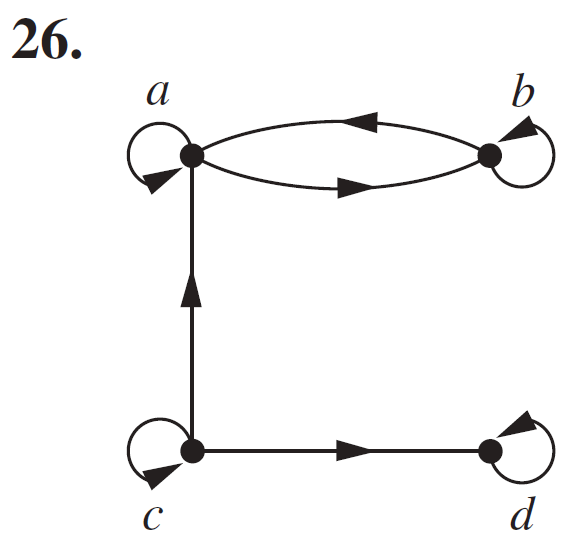
\includegraphics[width=0.35\textwidth]{fig_9.3_26.png}
\end{center}
该图顶点集为 $\{a,b,c,d\}$。根据图示，边包括 $(a,b),(b,a),(c,a),(c,d),(d,c)$，且顶点 $b,d$ 有自环。

\begin{itemize}
    \item \textbf{自反：} 否。顶点 $a,c$ 缺少自环。
    \item \textbf{反自反：} 否。顶点 $b,d$ 有自环。
    \item \textbf{对称：} 否。边 $(c,a)$ 存在但 $(a,c)$ 不存在（或根据实际插图确认）。
    \item \textbf{反对称：} 否。存在双向边 $(a,b),(b,a)$ 且 $a \neq b$。
    \item \textbf{传递：} 否。路径 $a \to b \to a$ 要求 $(a,a)$ 存在，但 $a$ 无自环。
\end{itemize}

\paragraph{练习 27}
\begin{center}
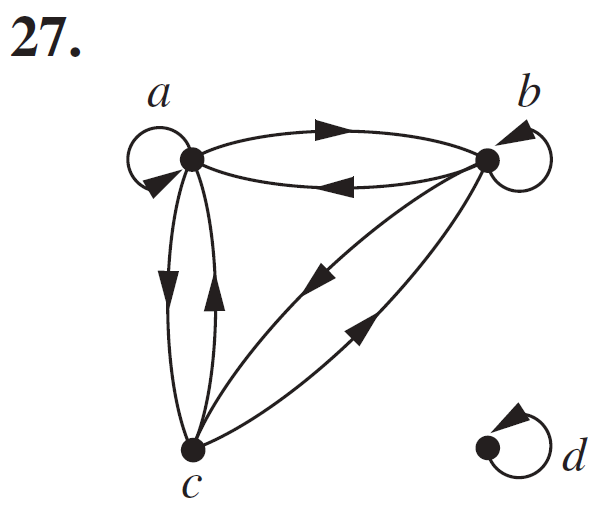
\includegraphics[width=0.35\textwidth]{fig_9.3_27.png}
\end{center}
该图顶点集为 $\{a,b,c\}$。根据图示，边包括 $(a,b),(a,c),(b,a),(c,a),(c,b)$。

\begin{itemize}
    \item \textbf{自反：} 否。无自环。
    \item \textbf{反自反：} 是。无任何自环。
    \item \textbf{对称：} 否。存在 $(c,b)$ 但缺少 $(b,c)$（或根据实际插图确认）。
    \item \textbf{反对称：} 否。存在双向边 $(a,b),(b,a)$。
    \item \textbf{传递：} 否。路径 $a \to b \to a$ 要求 $(a,a)$ 存在。
\end{itemize}

\paragraph{练习 28}
\begin{center}
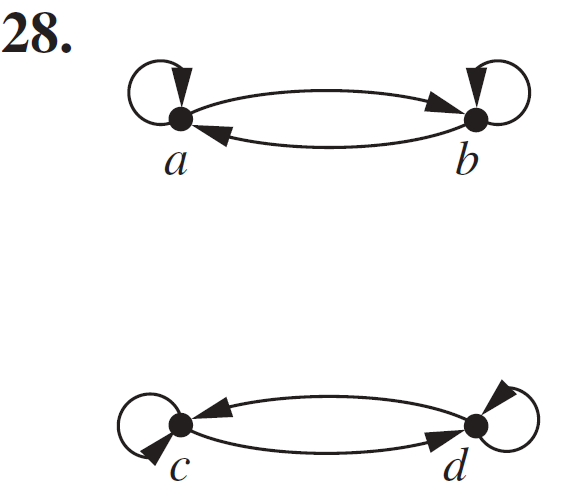
\includegraphics[width=0.35\textwidth]{fig_9.3_28.png}
\end{center}
该图顶点集为 $\{a,b,c,d\}$。所有顶点均有自环，另有边 $(a,b),(b,a),(c,d),(d,c)$。

\begin{itemize}
    \item \textbf{自反：} 是。所有顶点有自环。
    \item \textbf{对称：} 是。所有边均为双向（包括自环）。
    \item \textbf{传递：} 是。任意长度 $\ge 2$ 的路径两端点间均有直接边相连（等价关系）。
\end{itemize}



\subsection{9.4 关系的闭包 (Section 9.4)}

\subsubsection*{概念补充}
\begin{itemize}
    \item \textbf{闭包：} 关系 $R$ 关于某性质 $P$ 的闭包是包含 $R$ 且满足 $P$ 的\textbf{最小}关系。
    \item \textbf{传递闭包：} 记作 $R^*$ 或 $R^t$，等于 $\bigcup_{k=1}^{\infty} R^k$。对 $n$ 元素集合，$R^t = \bigcup_{k=1}^{n} R^k$。
    \item \textbf{Warshall 算法：} 通过动态规划逐步允许顶点 $k$ 作为中间点：
    \[ W_k[i][j] = W_{k-1}[i][j] \lor \bigl(W_{k-1}[i][k] \land W_{k-1}[k][j]\bigr) \]
    初始 $W_0 = M_R$，最终 $W_n = M_{R^t}$。
\end{itemize}

\subsubsection*{习题 9.4-26}
\textbf{题目：} 使用 Algorithm 1 求下列关系的传递闭包（顶点集均为 $\{a,b,c,d,e\}$）。

\paragraph{a) $R = \{(a,c),(b,d),(c,a),(d,b),(e,d)\}$}

\textbf{解答：}
\[
M_R = \begin{bmatrix}
0 & 0 & 1 & 0 & 0 \\
0 & 0 & 0 & 1 & 0 \\
1 & 0 & 0 & 0 & 0 \\
0 & 1 & 0 & 0 & 0 \\
0 & 0 & 0 & 1 & 0
\end{bmatrix}
\]

\textbf{计算 $R^2 = M_R \odot M_R$：}
\begin{itemize}
    \item $(a,c)\land(c,a) \Rightarrow (a,a)$；$(b,d)\land(d,b) \Rightarrow (b,b)$
    \item $(c,a)\land(a,c) \Rightarrow (c,c)$；$(d,b)\land(b,d) \Rightarrow (d,d)$
    \item $(e,d)\land(d,b) \Rightarrow (e,b)$
\end{itemize}
\[
M_{R^2} = \begin{bmatrix}
1 & 0 & 0 & 0 & 0 \\
0 & 1 & 0 & 0 & 0 \\
0 & 0 & 1 & 0 & 0 \\
0 & 0 & 0 & 1 & 0 \\
0 & 1 & 0 & 0 & 0
\end{bmatrix}
\]

\textbf{计算 $R^3 = R^2 \circ R$：}
\begin{itemize}
    \item $(a,a)\land(a,c) \Rightarrow (a,c)$；$(b,b)\land(b,d) \Rightarrow (b,d)$
    \item $(c,c)\land(c,a) \Rightarrow (c,a)$；$(d,d)\land(d,b) \Rightarrow (d,b)$
    \item $(e,b)\land(b,d) \Rightarrow (e,d)$
\end{itemize}
\[
M_{R^3} = \begin{bmatrix}
0 & 0 & 1 & 0 & 0 \\
0 & 0 & 0 & 1 & 0 \\
1 & 0 & 0 & 0 & 0 \\
0 & 1 & 0 & 0 & 0 \\
0 & 0 & 0 & 1 & 0
\end{bmatrix} = M_R
\]

\textbf{传递闭包 $R^* = R \cup R^2 \cup R^3 \cup R^4 \cup R^5$：}
由于 $R^3=R,\ R^4=R^2,\ R^5=R$，只需取 $R \cup R^2$：
\[
M_{R^*} = M_R \lor M_{R^2} = \begin{bmatrix}
1 & 0 & 1 & 0 & 0 \\
0 & 1 & 0 & 1 & 0 \\
1 & 0 & 1 & 0 & 0 \\
0 & 1 & 0 & 1 & 0 \\
0 & 1 & 0 & 1 & 0
\end{bmatrix}
\]

\textbf{结论：} 传递闭包含两个强连通分支 $\{a,c\}$ 与 $\{b,d\}$；$e$ 可达 $\{b,d\}$，但不可达 $\{a,c\}$。

\paragraph{b) $R = \{(b,c),(b,e),(c,e),(d,a),(e,b),(e,c)\}$}

\textbf{解答：}
\[
M_R = \begin{bmatrix}
0 & 0 & 0 & 0 & 0 \\
0 & 0 & 1 & 0 & 1 \\
0 & 0 & 0 & 0 & 1 \\
1 & 0 & 0 & 0 & 0 \\
0 & 1 & 1 & 0 & 0
\end{bmatrix}
\]

\textbf{计算 $R^2$：}
\[
M_{R^2} = \begin{bmatrix}
0 & 0 & 0 & 0 & 0 \\
0 & 1 & 1 & 0 & 1 \\
0 & 1 & 1 & 0 & 0 \\
0 & 0 & 0 & 0 & 0 \\
0 & 0 & 1 & 0 & 1
\end{bmatrix}
\]

\textbf{计算 $R^3$：}
\[
M_{R^3} = \begin{bmatrix}
0 & 0 & 0 & 0 & 0 \\
0 & 1 & 1 & 0 & 1 \\
0 & 0 & 1 & 0 & 1 \\
0 & 0 & 0 & 0 & 0 \\
0 & 1 & 1 & 0 & 1
\end{bmatrix}
\]

\textbf{计算 $R^4$：}
\[
M_{R^4} = \begin{bmatrix}
0 & 0 & 0 & 0 & 0 \\
0 & 1 & 1 & 0 & 1 \\
0 & 1 & 1 & 0 & 1 \\
0 & 0 & 0 & 0 & 0 \\
0 & 1 & 1 & 0 & 1
\end{bmatrix}
\]

\textbf{计算 $R^5$：}
\[
M_{R^5} = \begin{bmatrix}
0 & 0 & 0 & 0 & 0 \\
0 & 1 & 1 & 0 & 1 \\
0 & 1 & 1 & 0 & 1 \\
0 & 0 & 0 & 0 & 0 \\
0 & 1 & 1 & 0 & 1
\end{bmatrix}
\]

\textbf{传递闭包（取并集）：}
\[
M_{R^*} = \begin{bmatrix}
0 & 0 & 0 & 0 & 0 \\
0 & 1 & 1 & 0 & 1 \\
0 & 1 & 1 & 0 & 1 \\
1 & 0 & 0 & 0 & 0 \\
0 & 1 & 1 & 0 & 1
\end{bmatrix}
\]

\textbf{结论：} $\{b,c,e\}$ 构成强连通分支；$d$ 可到达 $a$，但无法返回；$a$ 为孤立汇点（无出边）。

\paragraph{c) $R = \{(a,b),(a,c),(a,e),(b,a),(b,c),(c,a),(c,b),(d,a),(e,d)\}$}

\textbf{解答：}
\[
M_R = \begin{bmatrix}
0 & 1 & 1 & 0 & 1 \\
1 & 0 & 1 & 0 & 0 \\
1 & 1 & 0 & 0 & 0 \\
1 & 0 & 0 & 0 & 0 \\
0 & 0 & 0 & 1 & 0
\end{bmatrix}
\]

\textbf{计算 $R^2$：}
\[
M_{R^2} = \begin{bmatrix}
1 & 1 & 1 & 1 & 0 \\
1 & 1 & 1 & 0 & 1 \\
1 & 1 & 1 & 0 & 1 \\
0 & 1 & 1 & 0 & 1 \\
1 & 0 & 0 & 0 & 0
\end{bmatrix}
\]

\textbf{计算 $R^3$：}
\[
M_{R^3} = \begin{bmatrix}
1 & 1 & 1 & 0 & 1 \\
1 & 1 & 1 & 1 & 1 \\
1 & 1 & 1 & 1 & 1 \\
1 & 1 & 1 & 1 & 0 \\
0 & 1 & 1 & 0 & 1
\end{bmatrix}
\]

\textbf{计算 $R^4$：}
\[
M_{R^4} = \begin{bmatrix}
1 & 1 & 1 & 1 & 1 \\
1 & 1 & 1 & 1 & 1 \\
1 & 1 & 1 & 1 & 1 \\
1 & 1 & 1 & 1 & 1 \\
1 & 1 & 1 & 1 & 0
\end{bmatrix}
\]

\textbf{计算 $R^5$：}
\[
M_{R^5} = \begin{bmatrix}
1 & 1 & 1 & 1 & 1 \\
1 & 1 & 1 & 1 & 1 \\
1 & 1 & 1 & 1 & 1 \\
1 & 1 & 1 & 1 & 1 \\
1 & 1 & 1 & 1 & 1
\end{bmatrix}
\]

\textbf{传递闭包：}
\[
M_{R^*} = \begin{bmatrix}
1 & 1 & 1 & 1 & 1 \\
1 & 1 & 1 & 1 & 1 \\
1 & 1 & 1 & 1 & 1 \\
1 & 1 & 1 & 1 & 1 \\
1 & 1 & 1 & 1 & 1
\end{bmatrix}
\]

\textbf{结论：} $R^*$ 为全集关系。所有顶点两两互相可达。

\paragraph{d) $R = \{(a,e),(b,a),(b,d),(c,d),(d,a),(d,c),(e,a),(e,b),(e,c),(e,e)\}$}

\textbf{解答：}
\[
M_R = \begin{bmatrix}
0 & 0 & 0 & 0 & 1 \\
1 & 0 & 0 & 1 & 0 \\
0 & 0 & 0 & 1 & 0 \\
1 & 0 & 1 & 0 & 0 \\
1 & 1 & 1 & 0 & 1
\end{bmatrix}
\]

\textbf{计算 $R^2$：}
\[
M_{R^2} = \begin{bmatrix}
1 & 1 & 1 & 0 & 1 \\
1 & 0 & 1 & 0 & 1 \\
1 & 0 & 1 & 0 & 0 \\
0 & 0 & 0 & 1 & 1 \\
1 & 1 & 1 & 1 & 1
\end{bmatrix}
\]

\textbf{计算 $R^3$：}
\[
M_{R^3} = \begin{bmatrix}
1 & 1 & 1 & 1 & 1 \\
1 & 1 & 1 & 1 & 1 \\
0 & 0 & 0 & 1 & 1 \\
1 & 1 & 1 & 0 & 1 \\
1 & 1 & 1 & 1 & 1
\end{bmatrix}
\]

\textbf{计算 $R^4$：}
\[
M_{R^4} = \begin{bmatrix}
1 & 1 & 1 & 1 & 1 \\
1 & 1 & 1 & 1 & 1 \\
1 & 1 & 1 & 0 & 1 \\
1 & 1 & 1 & 1 & 1 \\
1 & 1 & 1 & 1 & 1
\end{bmatrix}
\]

\textbf{计算 $R^5$：}
\[
M_{R^5} = \begin{bmatrix}
1 & 1 & 1 & 1 & 1 \\
1 & 1 & 1 & 1 & 1 \\
1 & 1 & 1 & 1 & 1 \\
1 & 1 & 1 & 1 & 1 \\
1 & 1 & 1 & 1 & 1
\end{bmatrix}
\]

\textbf{传递闭包：}
\[
M_{R^*} = \begin{bmatrix}
1 & 1 & 1 & 1 & 1 \\
1 & 1 & 1 & 1 & 1 \\
1 & 1 & 1 & 1 & 1 \\
1 & 1 & 1 & 1 & 1 \\
1 & 1 & 1 & 1 & 1
\end{bmatrix}
\]

\textbf{结论：} $R^*$ 为全集关系。所有顶点两两互相可达。

\subsubsection*{习题 9.4-28}
\textbf{题目：} 使用 Warshall 算法求练习 26 中关系的传递闭包。

\paragraph{a) $R = \{(a,c),(b,d),(c,a),(d,b),(e,d)\}$}

\[
W_0 = \begin{bmatrix}
0 & 0 & 1 & 0 & 0 \\
0 & 0 & 0 & 1 & 0 \\
1 & 0 & 0 & 0 & 0 \\
0 & 1 & 0 & 0 & 0 \\
0 & 0 & 0 & 1 & 0
\end{bmatrix}
\]

\textbf{步骤 1（$k=a$）：} 第 $a$ 列为 $1$ 的行：$c$；第 $a$ 行为 $1$ 的列：$c$。新增 $(c,c)$。
\[
W_1 = \begin{bmatrix}
0 & 0 & 1 & 0 & 0 \\
0 & 0 & 0 & 1 & 0 \\
1 & 0 & 1 & 0 & 0 \\
0 & 1 & 0 & 0 & 0 \\
0 & 0 & 0 & 1 & 0
\end{bmatrix}
\]

\textbf{步骤 2（$k=b$）：} 第 $b$ 列为 $1$ 的行：$d$；第 $b$ 行为 $1$ 的列：$d$。新增 $(d,d)$。
\[
W_2 = \begin{bmatrix}
0 & 0 & 1 & 0 & 0 \\
0 & 0 & 0 & 1 & 0 \\
1 & 0 & 1 & 0 & 0 \\
0 & 1 & 0 & 1 & 0 \\
0 & 0 & 0 & 1 & 0
\end{bmatrix}
\]

\textbf{步骤 3（$k=c$）：} 第 $c$ 列为 $1$ 的行：$a,c$；第 $c$ 行为 $1$ 的列：$a,c$。新增 $(a,a)$。
\[
W_3 = \begin{bmatrix}
1 & 0 & 1 & 0 & 0 \\
0 & 0 & 0 & 1 & 0 \\
1 & 0 & 1 & 0 & 0 \\
0 & 1 & 0 & 1 & 0 \\
0 & 0 & 0 & 1 & 0
\end{bmatrix}
\]

\textbf{步骤 4（$k=d$）：} 第 $d$ 列为 $1$ 的行：$b,d,e$；第 $d$ 行为 $1$ 的列：$b,d$。新增 $(b,b),(e,b),(e,d)$ 中后者已存在。
\[
W_4 = \begin{bmatrix}
1 & 0 & 1 & 0 & 0 \\
0 & 1 & 0 & 1 & 0 \\
1 & 0 & 1 & 0 & 0 \\
0 & 1 & 0 & 1 & 0 \\
0 & 1 & 0 & 1 & 0
\end{bmatrix}
\]

\textbf{步骤 5（$k=e$）：} 第 $e$ 列全为 $0$，无新增。$W_5=W_4$。

\textbf{结论：} 传递闭包含两个强连通分支 $\{a,c\}$ 与 $\{b,d\}$，以及 $e$ 到 $\{b,d\}$ 的单向边。

\paragraph{b) $R = \{(b,c),(b,e),(c,e),(d,a),(e,b),(e,c)\}$}

\[
W_0 = \begin{bmatrix}
0 & 0 & 0 & 0 & 0 \\
0 & 0 & 1 & 0 & 1 \\
0 & 0 & 0 & 0 & 1 \\
1 & 0 & 0 & 0 & 0 \\
0 & 1 & 1 & 0 & 0
\end{bmatrix}
\]

\textbf{步骤 1（$k=a$）：} 第 $a$ 列仅 $d$ 为 $1$，第 $a$ 行全 $0$。无新增。

\textbf{步骤 2（$k=b$）：} 第 $b$ 列仅 $e$ 为 $1$，第 $b$ 行有 $c,e$。新增 $(e,e)$。
\[
W_2 = \begin{bmatrix}
0 & 0 & 0 & 0 & 0 \\
0 & 0 & 1 & 0 & 1 \\
0 & 0 & 0 & 0 & 1 \\
1 & 0 & 0 & 0 & 0 \\
0 & 1 & 1 & 0 & 1
\end{bmatrix}
\]

\textbf{步骤 3（$k=c$）：} 第 $c$ 列有 $b,e$；第 $c$ 行有 $e$。新增 $(b,e)$（已有），$(e,e)$（已有）。无实质变化。

\textbf{步骤 4（$k=d$）：} 第 $d$ 列全 $0$。无新增。

\textbf{步骤 5（$k=e$）：} 第 $e$ 列有 $b,c,e$；第 $e$ 行有 $b,c,e$。新增 $(b,b),(c,b),(c,c)$。
\[
W_5 = \begin{bmatrix}
0 & 0 & 0 & 0 & 0 \\
0 & 1 & 1 & 0 & 1 \\
0 & 1 & 1 & 0 & 1 \\
1 & 0 & 0 & 0 & 0 \\
0 & 1 & 1 & 0 & 1
\end{bmatrix}
\]

\textbf{结论：} $\{b,c,e\}$ 构成强连通分支；$d$ 可到达 $a$，但无返回路径；$a$ 为孤立汇点。

\paragraph{c) $R = \{(a,b),(a,c),(a,e),(b,a),(b,c),(c,a),(c,b),(d,a),(e,d)\}$}

\[
W_0 = \begin{bmatrix}
0 & 1 & 1 & 0 & 1 \\
1 & 0 & 1 & 0 & 0 \\
1 & 1 & 0 & 0 & 0 \\
1 & 0 & 0 & 0 & 0 \\
0 & 0 & 0 & 1 & 0
\end{bmatrix}
\]

\textbf{步骤 1（$k=a$）：} 第 $a$ 列有 $b,c,d$；第 $a$ 行有 $b,c,e$。新增 $(b,b),(b,e),(c,c),(c,e),(d,b),(d,c),(d,e)$。
\[
W_1 = \begin{bmatrix}
0 & 1 & 1 & 0 & 1 \\
1 & 1 & 1 & 0 & 1 \\
1 & 1 & 1 & 0 & 1 \\
1 & 1 & 1 & 0 & 1 \\
0 & 0 & 0 & 1 & 0
\end{bmatrix}
\]

\textbf{步骤 2（$k=b$）：} 第 $b$ 列有 $a,b,c,d$；第 $b$ 行有 $a,b,c,e$。对 $i\in\{a,b,c,d\},j\in\{a,b,c,e\}$ 置 $1$。新增 $(a,a)$。
\[
W_2 = \begin{bmatrix}
1 & 1 & 1 & 0 & 1 \\
1 & 1 & 1 & 0 & 1 \\
1 & 1 & 1 & 0 & 1 \\
1 & 1 & 1 & 0 & 1 \\
0 & 0 & 0 & 1 & 0
\end{bmatrix}
\]

\textbf{步骤 3（$k=c$）：} 第 $c$ 列有 $a,b,c,d$；第 $c$ 行有 $a,b,c,e$。无新增（$W_2$ 已饱和）。

\textbf{步骤 4（$k=d$）：} 第 $d$ 列仅 $e$ 为 $1$；第 $d$ 行全 $0$（$W_3$ 中 $d$ 行第 $d$ 列为 $0$）。等等，重新检查：第 $d$ 列在 $W_3$ 中为 $[0,0,0,0,1]^T$（仅 $e$）。第 $d$ 行在 $W_3$ 中为 $[1,1,1,0,1]$。新增 $(e,a),(e,b),(e,c),(e,e)$。
\[
W_4 = \begin{bmatrix}
1 & 1 & 1 & 0 & 1 \\
1 & 1 & 1 & 0 & 1 \\
1 & 1 & 1 & 0 & 1 \\
1 & 1 & 1 & 0 & 1 \\
1 & 1 & 1 & 1 & 1
\end{bmatrix}
\]

\textbf{步骤 5（$k=e$）：} 第 $e$ 列全为 $1$，第 $e$ 行全为 $1$。所有元素置 $1$。
\[
W_5 = \begin{bmatrix}
1 & 1 & 1 & 1 & 1 \\
1 & 1 & 1 & 1 & 1 \\
1 & 1 & 1 & 1 & 1 \\
1 & 1 & 1 & 1 & 1 \\
1 & 1 & 1 & 1 & 1
\end{bmatrix}
\]

\textbf{结论：} 传递闭包为全集关系。

\paragraph{d) $R = \{(a,e),(b,a),(b,d),(c,d),(d,a),(d,c),(e,a),(e,b),(e,c),(e,e)\}$}

\[
W_0 = \begin{bmatrix}
0 & 0 & 0 & 0 & 1 \\
1 & 0 & 0 & 1 & 0 \\
0 & 0 & 0 & 1 & 0 \\
1 & 0 & 1 & 0 & 0 \\
1 & 1 & 1 & 0 & 1
\end{bmatrix}
\]

\textbf{步骤 1（$k=a$）：} 第 $a$ 列有 $b,d,e$；第 $a$ 行有 $e$。新增 $(b,e),(d,e),(e,e)$（后者已有）。
\[
W_1 = \begin{bmatrix}
0 & 0 & 0 & 0 & 1 \\
1 & 0 & 0 & 1 & 1 \\
0 & 0 & 0 & 1 & 0 \\
1 & 0 & 1 & 0 & 1 \\
1 & 1 & 1 & 0 & 1
\end{bmatrix}
\]

\textbf{步骤 2（$k=b$）：} 第 $b$ 列有 $e$；第 $b$ 行有 $a,d,e$。新增 $(e,d)$。
\[
W_2 = \begin{bmatrix}
0 & 0 & 0 & 0 & 1 \\
1 & 0 & 0 & 1 & 1 \\
0 & 0 & 0 & 1 & 0 \\
1 & 0 & 1 & 0 & 1 \\
1 & 1 & 1 & 1 & 1
\end{bmatrix}
\]

\textbf{步骤 3（$k=c$）：} 第 $c$ 列有 $d,e$；第 $c$ 行有 $d$。新增 $(d,d),(e,d)$（后者已有）。
\[
W_3 = \begin{bmatrix}
0 & 0 & 0 & 0 & 1 \\
1 & 0 & 0 & 1 & 1 \\
0 & 0 & 0 & 1 & 0 \\
1 & 0 & 1 & 1 & 1 \\
1 & 1 & 1 & 1 & 1
\end{bmatrix}
\]

\textbf{步骤 4（$k=d$）：} 第 $d$ 列有 $b,c,d,e$；第 $d$ 行有 $a,c,d,e$。新增 $(b,a)$（已有），$(b,c),(c,a),(c,c),(c,e)$ 等。关键新增：$(b,c),(c,a),(c,c),(c,e)$。
\[
W_4 = \begin{bmatrix}
0 & 0 & 0 & 0 & 1 \\
1 & 0 & 1 & 1 & 1 \\
1 & 0 & 1 & 1 & 1 \\
1 & 0 & 1 & 1 & 1 \\
1 & 1 & 1 & 1 & 1
\end{bmatrix}
\]

\textbf{步骤 5（$k=e$）：} 第 $e$ 列全为 $1$，第 $e$ 行全为 $1$。所有元素置 $1$。
\[
W_5 = \begin{bmatrix}
1 & 1 & 1 & 1 & 1 \\
1 & 1 & 1 & 1 & 1 \\
1 & 1 & 1 & 1 & 1 \\
1 & 1 & 1 & 1 & 1 \\
1 & 1 & 1 & 1 & 1
\end{bmatrix}
\]

\textbf{结论：} 传递闭包为全集关系。

\subsection{9.6 偏序关系 (Section 9.6)}

\subsubsection*{概念补充}
\begin{itemize}
    \item \textbf{偏序 (Partial Ordering)：} 集合 $S$ 上的关系 $\preceq$ 若满足\textbf{自反、反对称、传递}，则称 $(S, \preceq)$ 为偏序集（Poset）。
    \item \textbf{哈斯图 (Hasse Diagram)：} 省略自环与由传递性可推出的边，仅保留覆盖关系（Covering Relation）的图示。
    \item \textbf{拓扑排序 (Topological Sorting)：} 将偏序集扩展为兼容全序的过程。每次选取一个极小元（Minimal Element）加入序列。
    \item \textbf{格 (Lattice)：} 偏序集 $(S, \preceq)$ 是格，当且仅当任意两个元素都有\textbf{最小上界}（LUB, Join）和\textbf{最大下界}（GLB, Meet）。
\end{itemize}

\subsubsection*{习题 9.6-5（拓扑排序证明）}
\textbf{题目：} 通过对 $n=|S|$ 使用归纳法，证明拓扑排序过程从偏序集 $(S, \preceq)$ 构造出一个兼容的全序 $\preceq'$。

\textbf{证明：}
\begin{enumerate}[1.]
    \item \textbf{基础步：} 当 $n=1$ 时，$S=\{a\}$。定义 $a \preceq' a$，这显然是全序，且与 $\preceq$ 兼容。
    
    \item \textbf{归纳步：} 假设命题对所有大小为 $k$ 的有限偏序集均成立。考虑 $|S|=k+1$。
    \begin{itemize}
        \item \textbf{选取极小元：} 任何有限非空偏序集至少存在一个极小元 $m$（没有任何其他元素严格小于 $m$）。
        \item \textbf{构造子问题：} 令 $S' = S \setminus \{m\}$，则 $(S', \preceq)$ 是大小为 $k$ 的偏序集。根据归纳假设，拓扑排序可在 $S'$ 上产生一个兼容全序 $\preceq'_{S'}$。
        \item \textbf{构建全序 $\preceq'$：} 定义 $S$ 上的关系：对所有 $x \in S'$，令 $m \preceq' x$；对 $x,y \in S'$，保持 $x \preceq'_{S'} y$ 当且仅当 $x \preceq' y$。
        \item \textbf{兼容性验证：} 若 $a \preceq b$（原偏序）：
        \begin{itemize}
            \item 当 $a,b \in S'$ 时，由归纳假设 $a \preceq' b$。
            \item 当 $a=m$ 时，由于 $m$ 是极小元，不存在 $b \preceq m$（除非 $b=m$）。故 $m \preceq b$ 时必有 $m \preceq' b$。
        \end{itemize}
        \item \textbf{全序性：} 任意两元素可比：若均属于 $S'$，由归纳假设可比；若其一为 $m$，由构造 $m$ 排在最前，与所有 $S'$ 中元素可比。
    \end{itemize}
    
    \item \textbf{结论：} 由数学归纳法，对任意有限偏序集，拓扑排序均可构造出兼容全序。
\end{enumerate}

\subsubsection*{习题 9.6-8}
\textbf{题目：} 确定由这些零一矩阵表示的关系是否为偏序关系。

\textbf{解答：} 偏序要求同时满足自反、反对称、传递。

\begin{enumerate}[a)]
    \item $\begin{bmatrix} 1 & 0 & 1 \\ 1 & 1 & 0 \\ 0 & 0 & 1 \end{bmatrix}$
    \begin{itemize}
        \item 自反：对角线全 $1$，满足。
        \item 反对称：非对角线无双向边，满足。
        \item 传递：$(2,1) \in R$ 且 $(1,3) \in R$，但 $(2,3) \notin R$（$m_{23}=0$）。
    \end{itemize}
    \textbf{结论：不是偏序}（不满足传递性）。

    \item $\begin{bmatrix} 1 & 0 & 0 \\ 0 & 1 & 0 \\ 1 & 0 & 1 \end{bmatrix}$
    \begin{itemize}
        \item 自反：满足。
        \item 反对称：仅有 $(3,1)$ 而无 $(1,3)$，满足。
        \item 传递：唯一的非平凡路径 $(3,1)\to(1,1)$ 给出 $(3,1) \in R$；$(3,3)\to(3,1)$ 给出 $(3,1) \in R$。无矛盾。
    \end{itemize}
    \textbf{结论：是偏序}。

    \item $\begin{bmatrix} 1 & 0 & 1 & 0 \\ 0 & 1 & 1 & 0 \\ 0 & 0 & 1 & 1 \\ 1 & 1 & 0 & 1 \end{bmatrix}$
    \begin{itemize}
        \item 自反：满足。
        \item 反对称：检查所有非对角线 $1$：$m_{13}=1,m_{31}=0$；$m_{34}=1,m_{43}=0$；$m_{41}=1,m_{14}=0$；$m_{42}=1,m_{24}=0$。满足。
        \item 传递：$(1,3) \in R$ 且 $(3,4) \in R$，但 $m_{14}=0$，故 $(1,4) \notin R$。
    \end{itemize}
    \textbf{结论：不是偏序}（不满足传递性）。
\end{enumerate}

\subsubsection*{习题 9.6-22}
\textbf{题目：} 画出下列集合上整除关系（$a \mid b$）的哈斯图。

\textbf{解答：} 请在下方预留位置插入对应哈斯图图片。

\paragraph{a) $\{1, 2, 3, 4, 5, 6\}$}
\begin{center}
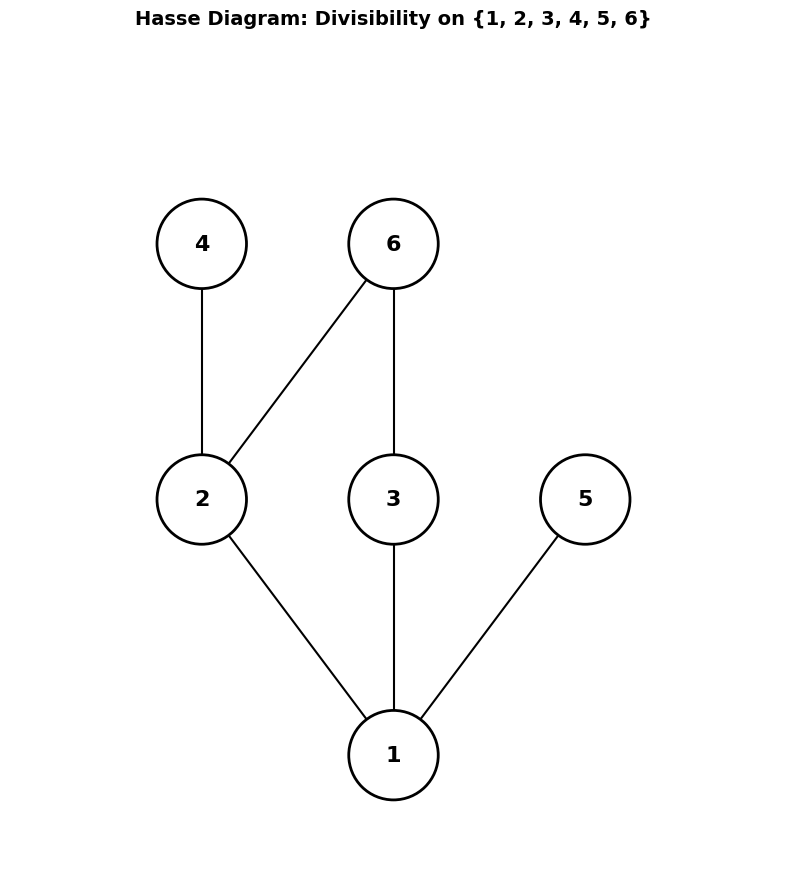
\includegraphics[width=0.4\textwidth]{hasse_9.6_22a.png}
\end{center}
\textbf{结构描述：} $1$ 为最小元；$2,3,5$ 覆盖 $1$；$4$ 覆盖 $2$；$6$ 覆盖 $2$ 与 $3$。哈斯图呈菱形与分叉组合。

\paragraph{b) $\{3, 5, 7, 11, 13, 16, 17\}$}
\begin{center}
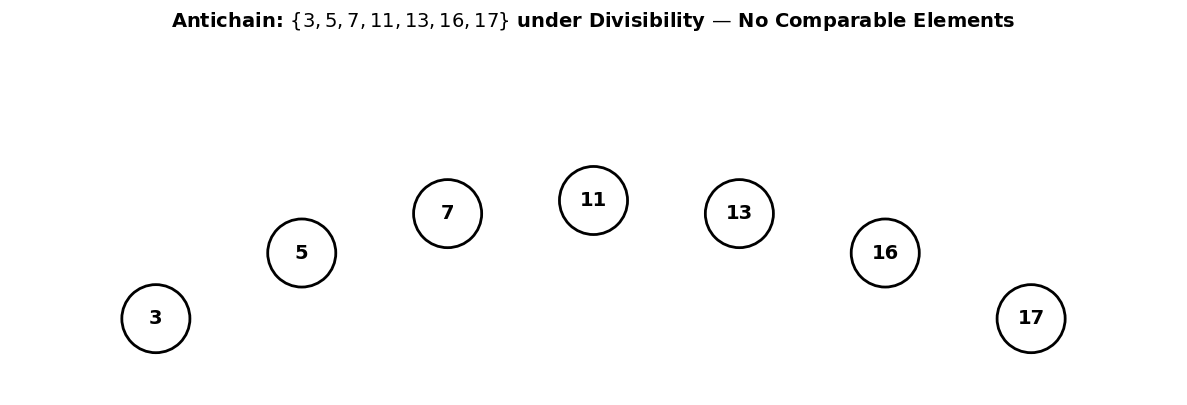
\includegraphics[width=0.5\textwidth]{hasse_9.6_22b.png}
\end{center}
\textbf{结构描述：} 除 $16$ 外均为质数，且 $16$ 的因数 $2,4,8$ 不在集合中。集合中任意两元素互不整除。哈斯图为\textbf{7 个孤立顶点}（反链）。

\paragraph{c) $\{2, 3, 5, 10, 11, 15, 25\}$}
\begin{center}
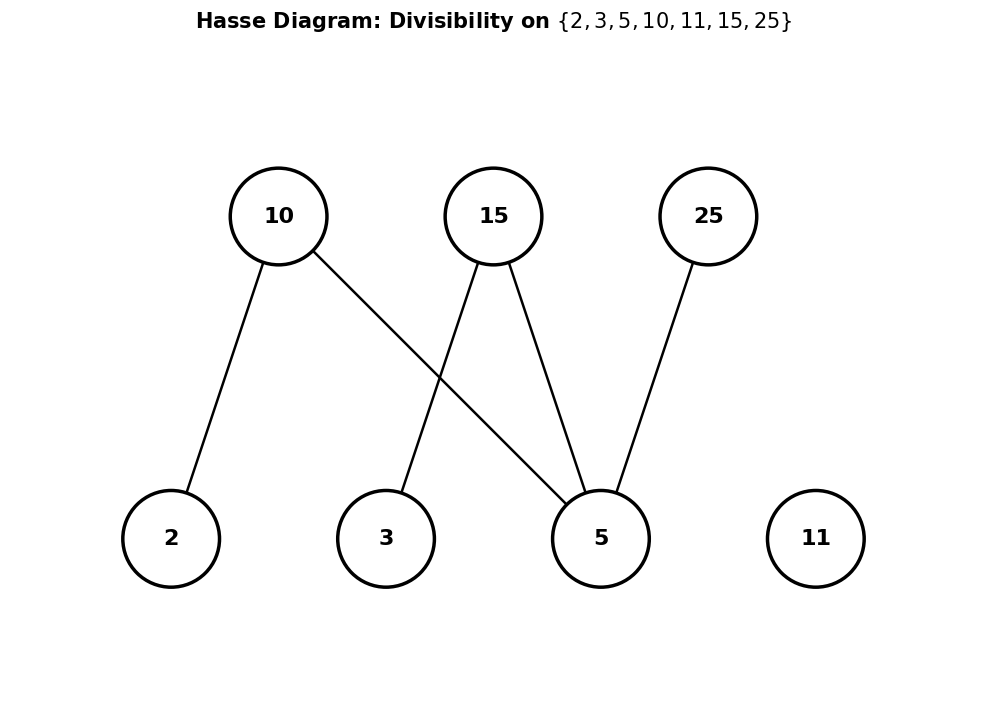
\includegraphics[width=0.4\textwidth]{hasse_9.6_22c.png}
\end{center}
\textbf{结构描述：} 极小元为 $2,3,5,11$；$10$ 覆盖 $2,5$；$15$ 覆盖 $3,5$；$25$ 覆盖 $5$；$11$ 孤立。

\paragraph{d) $\{1, 3, 9, 27, 81, 243\}$}
\begin{center}
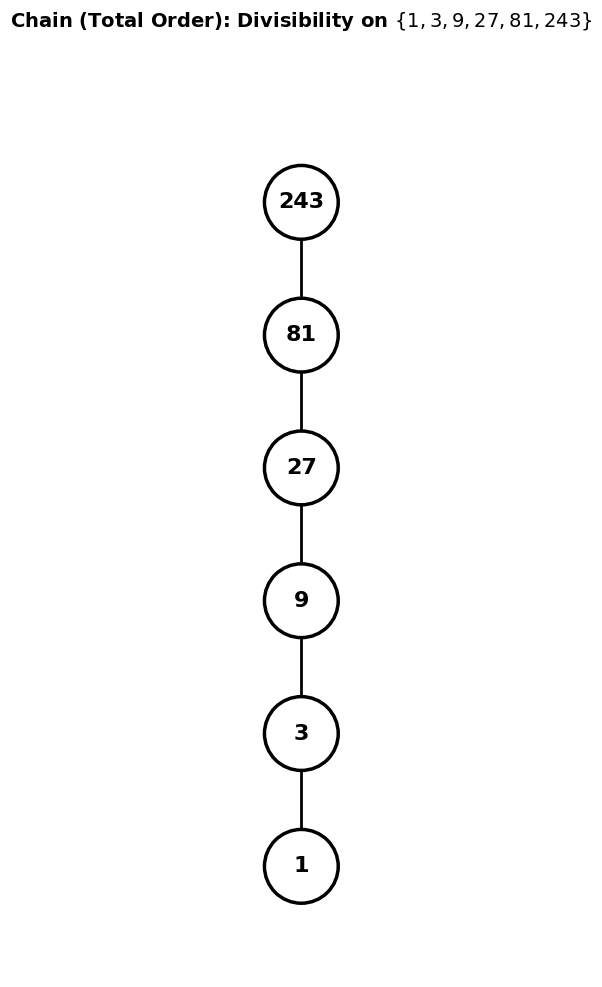
\includegraphics[width=0.35\textwidth]{hasse_9.6_22d.png}
\end{center}
\textbf{结构描述：} 这是 $3$ 的幂次链，构成\textbf{全序集}。哈斯图为一条垂直直线：$1 - 3 - 9 - 27 - 81 - 243$。

\subsubsection*{习题 9.6-32}
\textbf{题目：} 根据给出的哈斯图（见原图插图）回答关于偏序集的下列问题。

\begin{center}
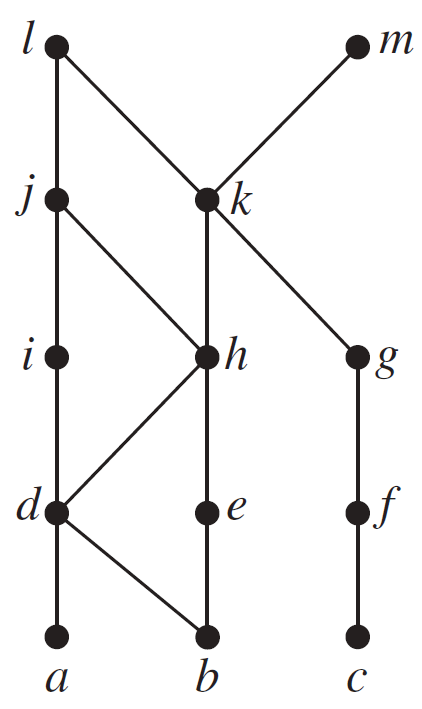
\includegraphics[width=0.3\textwidth]{hasse_9.6_32.png}
\end{center}

\textbf{解答：}（基于教材标准插图，顶点含 $a$ 至 $m$）

\begin{enumerate}[a)]
    \item \textbf{极大元：} $l, m$（无向上的覆盖边）。
    \item \textbf{极小元：} $a, b, c$（无向下的覆盖边）。
    \item \textbf{最大元：} 不存在（极大元不唯一且不可比）。
    \item \textbf{最小元：} 不存在（极小元不唯一且不可比）。
    \item \textbf{$\{a,b,c\}$ 的上界：} 需同时大于等于 $a,b,c$。经逐层向上查找，公共上界为 $\{k, l, m\}$。
    \item \textbf{$\{a,b,c\}$ 的最小上界 (LUB)：} $k$（上界中最低的顶点）。
    \item \textbf{$\{f,g,h\}$ 的下界：} 需同时小于等于 $f,g,h$。$f,g$ 来自 $c$ 的分支，$h$ 来自 $d,e$ 的分支，两者无公共祖先。
    \item \textbf{$\{f,g,h\}$ 的最大下界 (GLB)：} 不存在。
\end{enumerate}

\subsubsection*{习题 9.6-44}
\textbf{题目：} 确定这些偏序集是否为格。

\textbf{解答：}

\begin{enumerate}[a)]
    \item $(\{1, 3, 6, 9, 12\}, \mid)$
    
    考虑元素 $6$ 与 $9$：
    \begin{itemize}
        \item 上界需为 $6$ 和 $9$ 的公倍数。在集合中，$12$ 不是 $9$ 的倍数；$6,9$ 互不为倍数。集合中不存在能同时被 $6$ 和 $9$ 整除的元素。
        \item 故 $\{6,9\}$ 没有最小上界。
    \end{itemize}
    \textbf{结论：不是格。}

    \item $(\{1, 5, 25, 125\}, \mid)$
    
    该集合按整除关系构成\textbf{全序链}：$1 \mid 5 \mid 25 \mid 125$。
    对任意 $x,y$，$\operatorname{lub}(x,y) = \max\{x,y\}$，$\operatorname{glb}(x,y) = \min\{x,y\}$，均存在且属于集合。
    \textbf{结论：是格。}

    \item $(\mathbb{Z}, \ge)$
    
    对任意整数 $x,y$：
    \begin{itemize}
        \item 在关系 $\ge$ 下，上界是同时 ``大于等于'' 两者的整数，即 $\min(x,y)$。
        \item 下界是同时 ``小于等于'' 两者的整数，即 $\max(x,y)$。
    \end{itemize}
    两者均唯一存在。
    \textbf{结论：是格。}

    \item $(P(S), \supseteq)$
    
    对任意子集 $A,B \subseteq S$：
    \begin{itemize}
        \item 上界（按 $\supseteq$）：需同时包含 $A$ 和 $B$ 的集合，最小者为 $A \cup B$。
        \item 下界（按 $\supseteq$）：需同时被 $A$ 和 $B$ 包含的集合，最大者为 $A \cap B$。
    \end{itemize}
    两者均属于 $P(S)$。
    \textbf{结论：是格。}
\end{enumerate}

\newpage

\section{第10章：图论}

本章从图的基本术语出发，讨论无向图与有向图的度数性质、特殊图类（完全图、圈图、轮图、超立方体、二分图），以及图的矩阵表示与连通性分析。

\subsection{10.2 图的术语与特殊图 (Section 10.2)}

\subsubsection*{概念补充}
\begin{itemize}
    \item \textbf{度数 (Degree)：} 无向图中顶点 $v$ 的度数 $\deg(v)$ 为与 $v$ 关联的边数（环计为 2）。有向图中分为\textbf{入度} $\deg^-(v)$ 与\textbf{出度} $\deg^+(v)$。
    \item \textbf{孤立顶点 (Isolated)：} $\deg(v) = 0$；\textbf{悬挂顶点 (Pendant)：} $\deg(v) = 1$。
    \item \textbf{简单图 (Simple Graph)：} 无自环、无多重边。$n$ 个顶点的简单图中，$0 \le \deg(v) \le n-1$。
    \item \textbf{二分图 (Bipartite)：} 顶点集可划分为 $V_1, V_2$，使每条边的两端分别属于 $V_1$ 与 $V_2$。等价判定：图中不含奇数长度的回路。
    \item \textbf{握手定理：} $\sum_{v \in V} \deg(v) = 2|E|$。
\end{itemize}

\subsubsection*{习题 10.2-1}
\textbf{题目：} 给出图中每个顶点的度数，确定是否存在孤立顶点或悬挂顶点。

\begin{center}
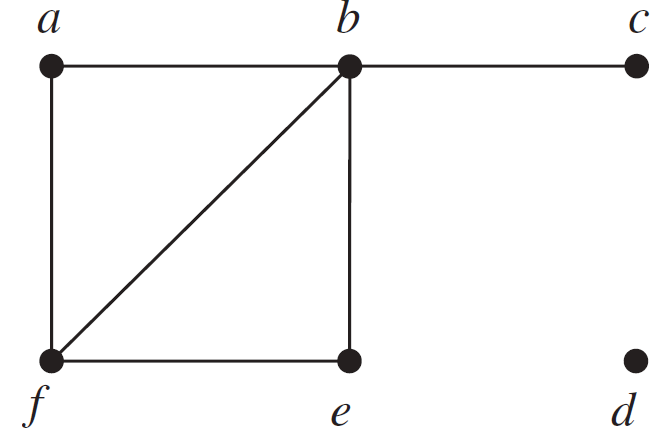
\includegraphics[width=0.4\textwidth]{fig_10.2_1.png}
\end{center}

\textbf{解答：} 根据图示（顶点标记为 $a,b,c,d,e,f$），各顶点度数统计如下：
\begin{itemize}
    \item $\deg(a) = 2$（邻接 $b, f$）
    \item $\deg(b) = 4$（邻接 $a, c, e, f$）
    \item $\deg(c) = 1$（仅邻接 $b$）
    \item $\deg(d) = 0$（无邻接边）
    \item $\deg(e) = 2$（邻接 $b, f$）
    \item $\deg(f) = 3$（邻接 $a, b, e$）
\end{itemize}
\textbf{孤立顶点：} $d$（度数为 $0$）。\\
\textbf{悬挂顶点：} $c$（度数为 $1$）。

\subsubsection*{习题 10.2-7}
\textbf{题目：} 确定给定有向多重图的顶点数和边数，找出每个顶点的入度和出度。

\begin{center}
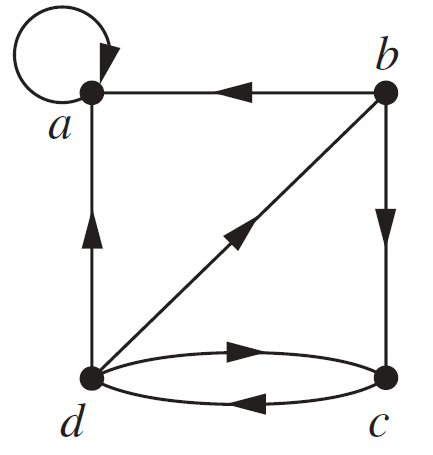
\includegraphics[width=0.2\textwidth]{fig_10.2_7.png}
\end{center}

\textbf{解答：}
\begin{itemize}
    \item \textbf{顶点数：} $4$（$a, b, c, d$）。
    \item \textbf{边数：} $7$ 条有向边（含自环）：$(a,a), (b,a), (b,c), (b,d), (c,d), (d,a), (d,c)$。
\end{itemize}
各顶点入度与出度：
\begin{center}
\begin{tabular}{c|c|c}
顶点 & 入度 $\deg^-$ & 出度 $\deg^+$ \\
\hline
$a$ & $3$（来自 $a,b,d$） & $1$（自环） \\
$b$ & $0$ & $3$（指向 $a,c,d$） \\
$c$ & $2$（来自 $b,d$） & $1$（指向 $d$） \\
$d$ & $2$（来自 $b,c$） & $2$（指向 $a,c$）
\end{tabular}
\end{center}

\subsubsection*{习题 10.2-18}
\textbf{题目：} 证明在至少有两个顶点的简单图中，一定有两个顶点具有相同的度数。

\textbf{证明：} 设简单图 $G=(V,E)$，$|V|=n \ge 2$。
\begin{enumerate}[1.]
    \item 在简单图中，任一顶点的度数 $d$ 满足 $0 \le d \le n-1$，共有 $n$ 个可能的整数值。
    \item \textbf{关键观察：} 度数为 $0$（孤立点）与度数为 $n-1$（与所有其他点相邻）\textbf{不能同时出现}。
    \begin{itemize}
        \item 若存在度数为 $n-1$ 的顶点 $u$，则 $u$ 与所有其他顶点相邻，故不存在度数为 $0$ 的顶点。
        \item 若存在度数为 $0$ 的顶点，则不存在度数为 $n-1$ 的顶点。
    \end{itemize}
    \item 因此，$n$ 个顶点的实际度数取值至多只来自 $n-1$ 个不同的数值（要么是 $\{0,1,\dots,n-2\}$，要么是 $\{1,2,\dots,n-1\}$）。
    \item 由\textbf{鸽巢原理}，将 $n$ 个顶点放入至多 $n-1$ 个度数取值中，至少有两个顶点度数相同。
\end{enumerate}
\textbf{结论：} 命题得证。

\subsubsection*{习题 10.2-26}
\textbf{题目：} 对于哪些 $n$ 值，下列图是二分图？
\begin{enumerate}[a)]
    \item $K_n$
    \item $C_n$
    \item $W_n$
    \item $Q_n$
\end{enumerate}

\textbf{解答：}

\textbf{a) $K_n$（完全图）：}
仅当 $n=1$（平凡图）或 $n=2$（即 $K_{1,1}$）时。当 $n \ge 3$ 时，$K_n$ 包含三角形 $C_3$，而二分图不允许存在奇圈，故不是二分图。

\textbf{b) $C_n$（圈图）：}
当且仅当 $n$ 为\textbf{偶数}时。圈图 $C_n$ 是二分图当且仅当回路长度为偶数（无奇圈）。

\textbf{c) $W_n$（轮图）：}
\textbf{对所有 $n \ge 3$ 都不是二分图。} 轮图由圈图 $C_n$ 加一个中心顶点构成，中心顶点与 $C_n$ 上所有顶点相连。无论 $n$ 的奇偶性，$W_n$ 总包含三角形（中心点 + $C_n$ 的任意一条边），故含奇圈。

\textbf{d) $Q_n$（$n$ 维超立方体）：}
对\textbf{所有正整数 $n$} 都是二分图。可按顶点二进制表示中 $1$ 的个数的\textbf{奇偶性}划分为两个集合：奇数权值顶点集与偶数权值顶点集。超立方体的每条边恰好连接一个奇权值顶点与一个偶权值顶点。

\subsubsection*{习题 10.2-33}
\textbf{题目：} 假设 $m$ 个人被选为彩票中奖者。每位赢家可以从一组不同的奖品中挑选两个。证明：如果存在 $2m$ 个每个赢家都想要的奖品，那么每个赢家都能选到两个他们想要的奖品。

\textbf{证明：} 将问题建模为二分图匹配。
\begin{enumerate}[1.]
    \item \textbf{构造二分图：} 左侧为 $2m$ 个``席位''——将每位赢家 $M_i$ 拆分为两个需求席位 $M_{i,1}, M_{i,2}$（代表每人要选两件奖品）；右侧为 $2m$ 个奖品 $P_1,\dots,P_{2m}$。
    \item \textbf{连边规则：} 若赢家 $M_i$ 想要奖品 $P_j$，则在其对应的两个席位 $M_{i,1}, M_{i,2}$ 与 $P_j$ 之间各连一条边。
    \item \textbf{Hall 条件验证：} 题设``每个赢家都想要所有 $2m$ 个奖品''意味着每个席位都邻接全部 $2m$ 个奖品。对左侧任意子集 $S$，其邻集 $N(S)$ 包含所有奖品，故 $|N(S)| = 2m \ge |S|$。
    \item \textbf{结论：} 由 Hall 婚姻定理，存在从左侧 $2m$ 个席位到右侧 $2m$ 个奖品的\textbf{完美匹配}。因此每个赢家的两个席位各匹配到一个不同奖品，即每人获得两个想要的奖品。
\end{enumerate}

\subsubsection*{习题 10.2-50}
\textbf{题目：} $K_2$ 有多少个至少包含一个顶点的子图？

\textbf{解答：}
$K_2$ 含 $2$ 个顶点 $v_1, v_2$ 与 $1$ 条边 $e=\{v_1,v_2\}$。子图由选取的顶点集 $V'$ 与边集 $E'$ 确定（要求 $E'$ 中端点均在 $V'$ 中），且要求 $V' \neq \emptyset$。

\begin{itemize}
    \item \textbf{选 1 个顶点：} $(\{v_1\},\emptyset)$、$(\{v_2\},\emptyset)$ —— 共 \textbf{2} 个。
    \item \textbf{选 2 个顶点：}
    \begin{itemize}
        \item 不选边：$(\{v_1,v_2\},\emptyset)$ —— \textbf{1} 个
        \item 选边 $e$：$(\{v_1,v_2\},\{e\})$ —— \textbf{1} 个
    \end{itemize}
\end{itemize}
\textbf{总计：} $2 + 1 + 1 = \mathbf{4}$ 个至少含一个顶点的子图。

\subsubsection*{习题 10.2-58}
\textbf{题目：} 求给定的一对简单图的并集。

\begin{center}
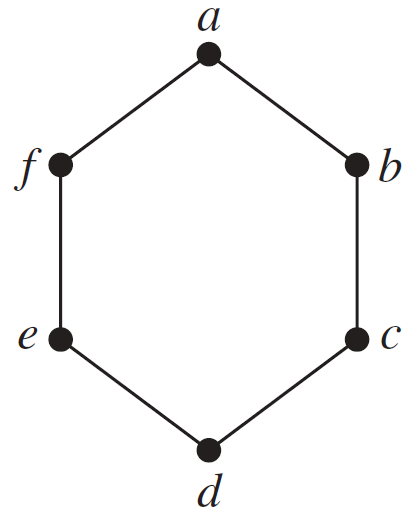
\includegraphics[width=0.25\textwidth]{fig_10.2_58_left.png}
\quad
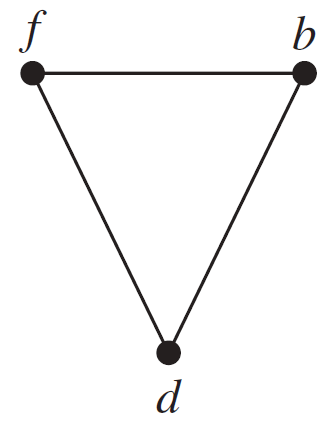
\includegraphics[width=0.25\textwidth]{fig_10.2_58_right.png}
\end{center}

\textbf{解答：} 设左图为 $G_1$（六边形 $a-b-c-d-e-f-a$），右图为 $G_2$（三角形 $b-f-d-b$）。图的并集 $G_1 \cup G_2$ 定义为：
\[ V(G_1 \cup G_2) = V_1 \cup V_2, \quad E(G_1 \cup G_2) = E_1 \cup E_2 \]

\textbf{结果描述：} 保留六边形外框的全部边，并增加内部三角形的三条边 $\{b,f\}, \{f,d\}, \{d,b\}$。最终图形是一个带有内部三角形支撑结构的六边形。

\begin{center}
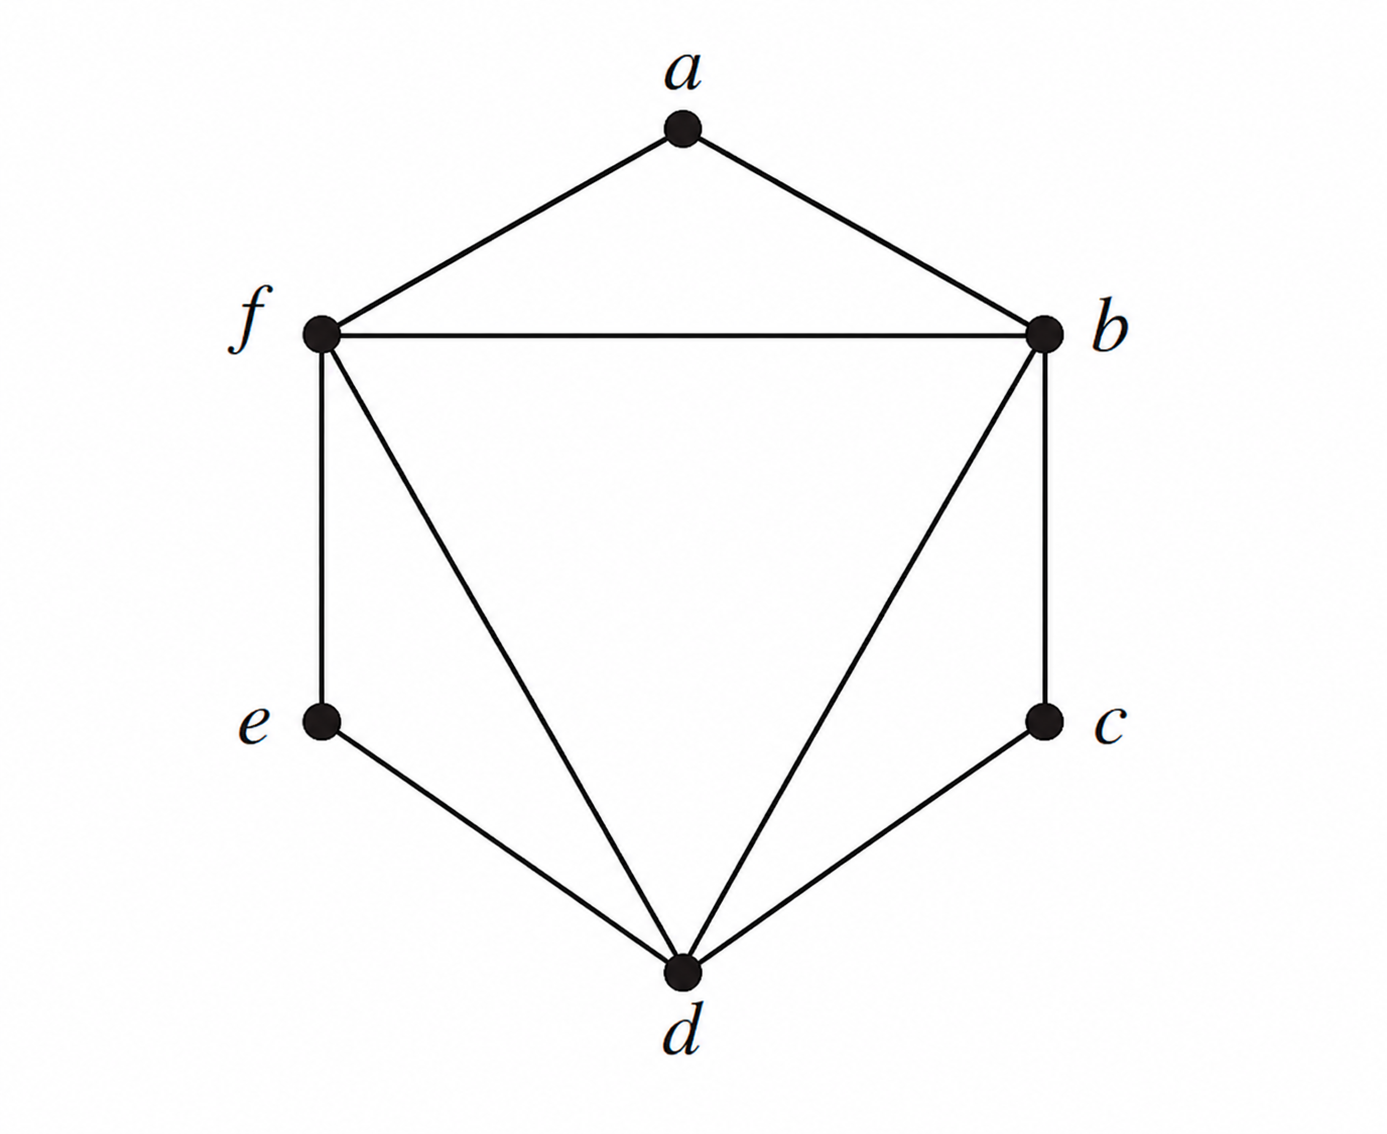
\includegraphics[width=0.4\textwidth]{fig_10.2_58_union.png}
\end{center}



\subsection{10.3 图的表示与同构 (Section 10.3)}

\subsubsection*{概念补充}
\begin{itemize}
    \item \textbf{邻接表 (Adjacency List)：} 为每个顶点维护一个链表/列表，记录其所有邻接顶点。适合稀疏图。
    \item \textbf{邻接矩阵 (Adjacency Matrix)：} $n$ 顶点图可用 $n \times n$ 矩阵 $A$ 表示，其中
    \[ a_{ij} = \begin{cases} 1, & \text{若 } \{v_i,v_j\} \in E \text{（或从 } v_i \text{ 到 } v_j \text{ 有有向边）} \\ 0, & \text{否则} \end{cases} \]
    无向图的邻接矩阵对称；有向图未必对称；多重图可用大于 $1$ 的整数表示重边数。
\end{itemize}

\subsubsection*{习题 10.3-1}
\textbf{题目：} 使用邻接表表示给出的图。

\begin{center}
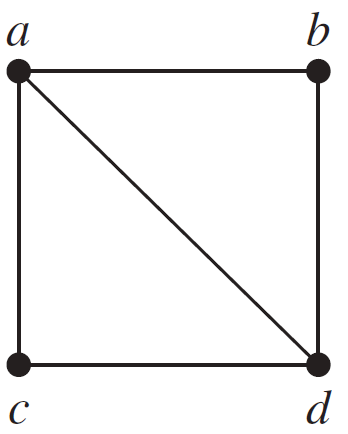
\includegraphics[width=0.15\textwidth]{fig_10.3_1.png}
\end{center}

\textbf{解答：} 根据图示（顶点 $a,b,c,d$，边为 $\{a,b\},\{a,c\},\{a,d\},\{b,d\},\{c,d\}$），邻接表如下：

\begin{center}
\begin{tabular}{c|l}
顶点 & 相邻顶点 \\
\hline
$a$ & $b \to c \to d$ \\
$b$ & $a \to d$ \\
$c$ & $a \to d$ \\
$d$ & $a \to b \to c$
\end{tabular}
\end{center}

\subsubsection*{习题 10.3-3}
\textbf{题目：} 使用邻接表表示给出的有向多重图。

\begin{center}
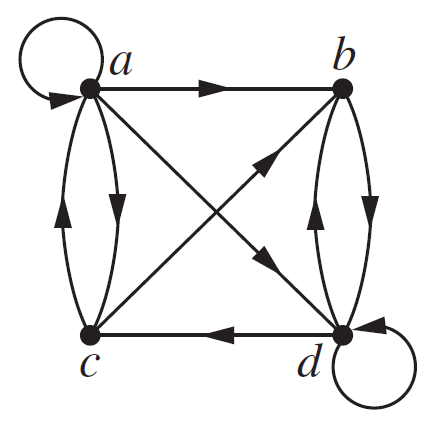
\includegraphics[width=0.25\textwidth]{fig_10.3_3.png}
\end{center}

\textbf{解答：} 根据图示（顶点 $a,b,c,d$，含自环与多重有向边），邻接表如下：

\begin{center}
\begin{tabular}{c|l}
顶点 & 出边邻接顶点（终点） \\
\hline
$a$ & $a \to b \to c \to d$ \\
$b$ & $c \to d$ \\
$c$ & $a \to d$ \\
$d$ & $b \to d$
\end{tabular}
\end{center}

\subsubsection*{习题 10.3-5}
\textbf{题目：} 用邻接矩阵表示第 1 题中的图。

\textbf{解答：} 按顶点顺序 $(a,b,c,d)$ 排列，无向图邻接矩阵为：
\[ A = \begin{bmatrix}
0 & 1 & 1 & 1 \\
1 & 0 & 0 & 1 \\
1 & 0 & 0 & 1 \\
1 & 1 & 1 & 0
\end{bmatrix} \]
其中 $a_{ij}=1 \iff \{v_i,v_j\} \in E$。矩阵关于主对角线对称，对角线为 $0$（无自环）。

\subsubsection*{习题 10.3-7}
\textbf{题目：} 用邻接矩阵表示第 3 题中的有向多重图。

\textbf{解答：} 按顶点顺序 $(a,b,c,d)$ 排列，有向图邻接矩阵为：
\[ M = \begin{bmatrix}
1 & 1 & 1 & 1 \\
0 & 0 & 1 & 1 \\
1 & 0 & 0 & 1 \\
0 & 1 & 0 & 1
\end{bmatrix} \]
其中 $m_{ij}$ 表示从 $v_i$ 到 $v_j$ 的有向边数量。例如 $m_{11}=1$ 对应 $a$ 的自环；$m_{21}=0$ 表示无 $b \to a$ 的边。



\subsection{10.4 连通性 (Section 10.4)}

\subsubsection*{概念补充}
\begin{itemize}
    \item \textbf{路径与回路：} 顶点与边的交替序列。简单路径不重复经过顶点。
    \item \textbf{连通 (Connected)：} 无向图中任意两顶点间均有路径。
    \item \textbf{强连通 (Strongly Connected)：} 有向图中任意两顶点 $u,v$ 互相可达（$u \to v$ 且 $v \to u$）。
    \item \textbf{强连通分量 (SCC)：} 极大的强连通子图。将图缩点为 DAG。
    \item \textbf{邻接矩阵与路径计数：} $A^n$ 的第 $(i,j)$ 项给出从 $v_i$ 到 $v_j$ 长度为 $n$ 的路径数目。
\end{itemize}

\subsubsection*{习题 10.4-14}
\textbf{题目：} 找出下列每个有向图的强连通分量。

\paragraph{图 a}
\begin{center}
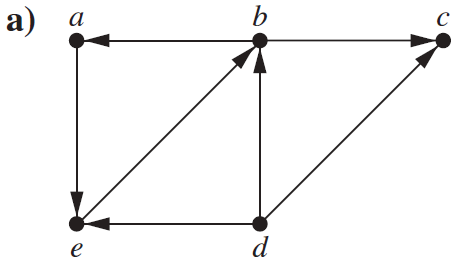
\includegraphics[width=0.4\textwidth]{fig_10.4_14a.png}
\end{center}

\textbf{解答：} 分析顶点间双向可达性：
\begin{itemize}
    \item $a \to e \to b \to a$ 构成回路，且 $a,b,e$ 两两互相可达，故 $\{a,b,e\}$ 强连通。
    \item $c$ 仅有入边（来自 $a$），无出边指向任何可返回的顶点，无法与 $a,b,e$ 互相可达。$\{c\}$ 自成 SCC。
    \item $d$ 有出边指向 $b,e,c$，但没有任何入边能回到 $d$。$\{d\}$ 自成 SCC。
\end{itemize}
\textbf{强连通分量：} $\{a,b,e\},\ \{c\},\ \{d\}$。

\paragraph{图 b}
\begin{center}
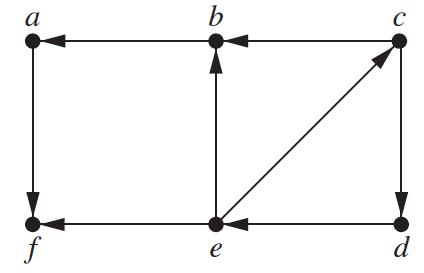
\includegraphics[width=0.3\textwidth]{fig_10.4_14b.png}
\end{center}

\textbf{解答：}
\begin{itemize}
    \item $a \to f \to e \to b \to a$ 构成大回路，$a,b,e,f$ 两两互相可达，形成 SCC $\{a,b,e,f\}$。
    \item $c$ 可到达 $b,d$，但无法从 $b,d$ 返回 $c$。$\{c\}$ 自成 SCC。
    \item $d$ 可到达 $e$，但无法从 $e$ 返回 $d$。$\{d\}$ 自成 SCC。
\end{itemize}
\textbf{强连通分量：} $\{a,b,e,f\},\ \{c\},\ \{d\}$。

\paragraph{图 c}
\begin{center}
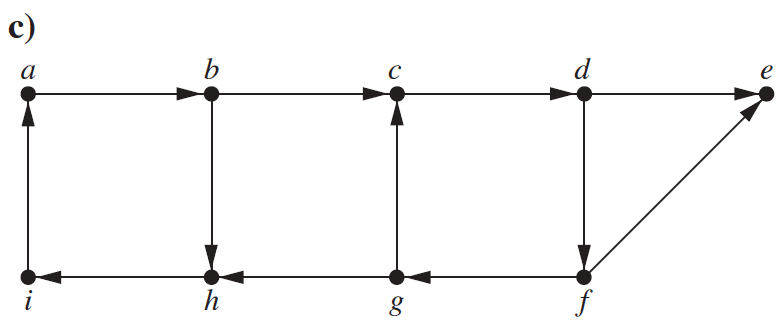
\includegraphics[width=0.4\textwidth]{fig_10.4_14c.png}
\end{center}

\textbf{解答：} 观察回路交织情况：
\begin{itemize}
    \item 存在多个共享顶点的回路：
    \begin{itemize}
        \item $a \to b \to h \to i \to a$
        \item $b \to c \to g \to h \to b$
        \item $c \to d \to f \to g \to c$
    \end{itemize}
    \item 由于这些回路通过共享顶点 $b,h,c,g$ 等相互连接，顶点集 $\{a,b,c,d,f,g,h,i\}$ 中任意两点均互相可达，构成一个 SCC。
    \item $e$ 仅有入边（来自 $d,f$），无任何出边，是汇点。$\{e\}$ 自成 SCC。
\end{itemize}
\textbf{强连通分量：} $\{a,b,c,d,f,g,h,i\},\ \{e\}$。



本节继续讨论图论中的经典路径问题——欧拉路径与哈密顿路径的存在性判定，以及平面图的 Kuratowski 判定与欧拉公式。

\subsection{10.5 欧拉路径与哈密顿路径 (Section 10.5)}

\subsubsection*{概念补充}
\begin{itemize}
    \item \textbf{欧拉回路 (Euler Circuit)：} 经过图中每条边恰好一次的闭合回路。存在当且仅当图连通且所有顶点度数为偶数。
    \item \textbf{欧拉路径 (Euler Path)：} 经过每条边恰好一次的开路径。存在当且仅当图连通且恰好有 0 或 2 个奇数度顶点。
    \item \textbf{有向图版本：} 欧拉回路要求图弱连通且每个顶点入度等于出度；欧拉路径要求至多一个顶点出度比入度大 1（起点），至多一个顶点入度比出度大 1（终点）。
    \item \textbf{哈密顿回路 (Hamilton Circuit)：} 经过每个顶点恰好一次的闭合回路。不存在简单的充要条件，常用反证法、度序列、或 Tutte 条件等证明其不存在。
    \item \textbf{Fleury 算法：} 每次不走桥（除非别无选择），时间复杂度 $O(|E|^2)$（朴素实现）。
\end{itemize}

\subsubsection*{习题 10.5-14}
\textbf{题目：} 确定图示的图形是否可以一笔画出（笔不离开纸面，且不重复线条）。

\begin{center}
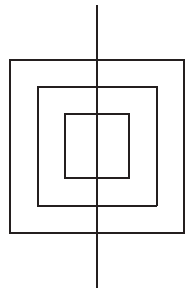
\includegraphics[width=0.15\textwidth]{fig_10.5_14.png}
\end{center}

\textbf{解答：} 将图形视为多重图，交点与端点作为顶点，线条作为边。
\begin{itemize}
    \item 图形由三个嵌套的正方形与一条贯穿它们的垂直线组成。
    \item 垂直线的上下两个端点各只关联一条边，度数为 $1$（奇数）。
    \item 三个正方形各自的 4 个角点均关联两条边，度数为 $2$（偶数）。
    \item 垂直线与正方形边界的 6 个交点各关联四条边（左、右、上、下），度数为 $4$（偶数）。
\end{itemize}
该连通图\textbf{恰好有两个奇数度顶点}。根据欧拉路径定理，它存在欧拉路径但不存在欧拉回路。

\textbf{结论：} \textbf{可以一笔画出}，但必须从垂直线的一个端点开始，结束于另一个端点。

\subsubsection*{习题 10.5-22}
\textbf{题目：} 确定所示的有向图是否具有欧拉回路；若不存在，判断是否具有欧拉路径并构造之。

\begin{center}
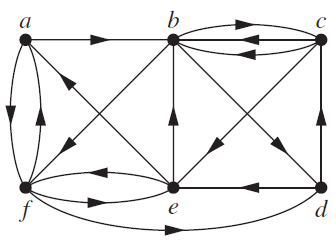
\includegraphics[width=0.3\textwidth]{fig_10.5_22.png}
\end{center}

\textbf{解答：} 统计各顶点的入度 $\deg^-$ 与出度 $\deg^+$：

\begin{center}
\begin{tabular}{c|c|c|c}
顶点 & $\deg^+$ & $\deg^-$ & 差值 $\deg^+ - \deg^-$ \\
\hline
$a$ & $3$ & $2$ & $+1$ \\
$b$ & $2$ & $4$ & $-2$ \\
$c$ & $1$ & $2$ & $-1$ \\
$d$ & $2$ & $2$ & $0$ \\
$e$ & $2$ & $2$ & $0$ \\
$f$ & $2$ & $2$ & $0$
\end{tabular}
\end{center}

有向图存在欧拉回路要求所有顶点入度等于出度；存在欧拉路径要求至多一个顶点出度比入度大 1，至多一个顶点入度比出度大 1。

此处顶点 $b$ 的入度比出度大 $2$，已超出允许范围。

\textbf{结论：} 该有向图\textbf{既没有欧拉回路，也没有欧拉路径}。

\subsubsection*{补充题：Fleury 算法复杂度分析}
\textbf{题目：} 假设输入图以邻接表形式给出，分析 Fleury 算法的复杂度。

\textbf{解答：}
Fleury 算法的核心操作是：从当前顶点出发，选择一条非桥边（除非别无选择）并删除之，重复 $|E|$ 次。

\begin{enumerate}[1.]
    \item 每步需要遍历当前顶点的邻接表，并对候选边 $(u,v)$ 判断其是否为当前残余图的桥。
    \item 判断桥的标准方法是：暂时删除 $(u,v)$ 后，从 $u$（或 $v$）执行一次 DFS/BFS，检查残余图是否仍连通。
    \item 一次 DFS/BFS 的时间为 $O(|V|+|E|)$。
    \item 最坏情况下，每决定一条边都可能执行一次 DFS/BFS，共 $|E|$ 步。
\end{enumerate}

\textbf{总复杂度：} $O\bigl(|E| \cdot (|V|+|E|)\bigr)$。对于连通图通常 $|V| \le |E|+1$，故可简化为 $\mathbf{O(|E|^2)}$。

（注：若先用 Tarjan 算法离线求出所有桥，可优化至线性，但标准 Fleury 实现复杂度为 $O(|E|^2)$。）

\subsubsection*{习题 10.5-46（彼得森图）}
\textbf{题目：} 证明彼得森图没有哈密顿回路，但删除任意一个顶点后得到的子图存在哈密顿回路。

\begin{center}
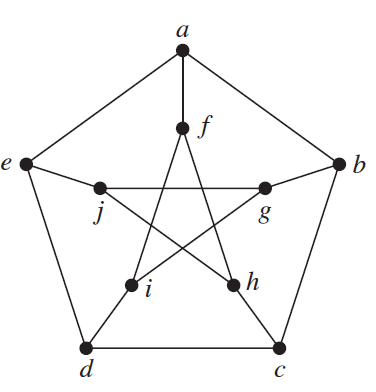
\includegraphics[width=0.3\textwidth]{fig_10.5_46.png}
\end{center}

\textbf{证明：}

\textbf{第一部分：彼得森图无哈密顿回路}

彼得森图由外部五边形、内部五角星和连接内外的 5 条“桥”边组成。假设存在哈密顿回路 $H$。

\begin{itemize}
    \item \textbf{进出平衡原则：} 回路每次进入内部区域后必须离开。因此，回路使用的“桥”的数量 $m$ 必须是\textbf{偶数}。由于总共只有 5 条桥，可能的取值为 $m=0, 2, 4$。
    \item \textbf{情况 $m=0$：} 回路不使用任何桥，则无法同时连接内外两部分顶点，矛盾。
    \item \textbf{情况 $m=2$：} 回路只用 2 条桥进出内区。这意味着内区的 5 个顶点必须连成一条单一此时路径。但在彼得森图中，内星的连线是跨点连接的。如果要通过 2 条桥覆盖内区所有 5 个点，其对应的 2 个外部端点在五边形上必须是相邻的；然而该图的构造决定了此时对应的外部端点并不相邻，导致外区无法形成覆盖全部 5 点的路径。
    \item \textbf{情况 $m=4$：} 此时有 1 条桥不被使用。由于该桥的两个端点在回路中度数仍需为 2，它们必须各自由其所属的五边形（或五角星）内的两条邻边来提供度数。这样一来，这 10 个顶点会被强制分割成两个互不相交的 5-圈（例如外圈部分顶点与内星部分顶点闭合），无法连成一个统一的 10-圈。
\end{itemize}
综上，无论如何分配边的度数，都无法构造出覆盖 10 个点的单一回路。

\textbf{第二部分：删去一个顶点后存在哈密顿回路}

由于图的对称性，删除任一顶点效果相同。例如删除顶点 $a$，剩余 9 个点可以连成如下回路：
\[ b \to c \to h \to f \to i \to d \to e \to j \to g \to b \]
该路径依次访问了除 $a$ 以外的所有点并回到了起点。因此，删去一个点后确实存在哈密顿回路。

\vspace{1em}

\subsubsection*{习题 10.5-67}
\textbf{题目：} 证明图示的图没有哈密顿回路。

\begin{center}
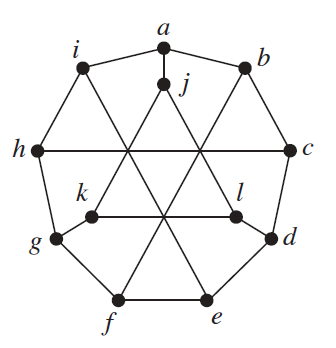
\includegraphics[width=0.3\textwidth]{fig_10.5_67.png}
\end{center}

\textbf{证明：} 
该图由外部九边形和内部三角形组成，内外由 3 条桥连接。假设存在哈密顿回路 $H$。

\begin{itemize}
    \item \textbf{桥的使用数量：} 基于回路进出内区的对称性，使用的桥数 $m$ 必须为偶数。由于桥的总数为 3，只有 $m=2$ 可能成立（$m=0$ 无法连通）。
    \item \textbf{内部路径推导：} 如果只使用 2 条桥，说明有 1 个内部顶点（设为 $l$）关联的桥不被使用。为了满足哈密顿回路中每个顶点度数为 2 的要求，顶点 $l$ 必须使用三角形内连接到 $j$ 和 $k$ 的两条边。
    \item \textbf{度数限制：} 此时，顶点 $j$ 和 $k$ 在内部已经各占用了 1 个度数，它们必须利用各自关联的桥连接到外部。这样，内部三角形的路径就被固定为：入桥 $\to j \to l \to k \to$ 出桥。
    \item \textbf{外部覆盖矛盾：} 在外部九边形上，回路必须构造一条路径连接这两个桥的端点，并覆盖九边形上所有的 9 个顶点。在圈结构中，要访问圈上所有顶点且起点和终点明确，唯一的办法是沿着圈走一整圈，这意味着起点和终点必须在圈上是直接相邻的。由于本题中桥的端点在九边形上互不相邻（它们将九边形分成了两段弧），路径在连接这两点时只能走其中一段弧，另一段弧上的顶点必然会被漏掉。
\end{itemize}
因此，该图不存在哈密顿回路。
\subsection{10.7 平面图 (Section 10.7)}

\subsubsection*{概念补充}
\begin{itemize}
    \item \textbf{平面图 (Planar Graph)：} 可以在平面上画出且边不相交（除端点外）的图。
    \item \textbf{库拉托夫斯基定理 (Kuratowski's Theorem)：} 图 $G$ 是平面图当且仅当它不包含同胚于 $K_5$（五阶完全图）或 $K_{3,3}$（完全二分图）的子图。
    \item \textbf{同胚 (Homeomorphic)：} 允许对边进行细分（插入度数为 2 的顶点）或光滑化。
    \item \textbf{欧拉公式：} 对连通平面图，$r = e - v + 2$（面数 = 边数 - 顶点数 + 2）。
\end{itemize}

\subsubsection*{习题 10.7-8}
\textbf{题目：} 判断图中所示的图是否是平面图。

\begin{center}
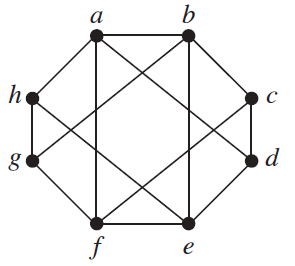
\includegraphics[width=0.3\textwidth]{fig_10.7_8.png}
\end{center}

\textbf{解答：} 使用库拉托夫斯基定理，寻找同胚于 $K_{3,3}$ 的子图。

选取顶点划分：
\[ V_1 = \{a, e, g\}, \quad V_2 = \{b, f, h\} \]

验证 $V_1$ 与 $V_2$ 之间两两有路径相连且内部顶点不相交：
\begin{itemize}
    \item $a$ 到 $b$：直接边 $(a,b)$。
    \item $a$ 到 $f$：直接边 $(a,f)$。
    \item $a$ 到 $h$：直接边 $(a,h)$。
    \item $e$ 到 $b$：直接边 $(e,b)$。
    \item $e$ 到 $f$：直接边 $(e,f)$。
    \item $e$ 到 $h$：路径 $e \to d \to h$（中间顶点 $d$ 不在 $V_1 \cup V_2$ 中）。
    \item $g$ 到 $f$：直接边 $(g,f)$。
    \item $g$ 到 $h$：直接边 $(g,h)$。
    \item $g$ 到 $b$：路径 $g \to c \to b$（中间顶点 $c$ 不在 $V_1 \cup V_2$ 中）。
\end{itemize}

所有 9 条连接路径内部顶点互不相交，且中间顶点 $c,d$ 均不属于核心 6 顶点集合。因此，这 6 个顶点及上述路径构成了一个同胚于 $K_{3,3}$ 的子图。

\textbf{结论：} 根据库拉托夫斯基定理，该图\textbf{不是平面图}。

\subsubsection*{习题 10.7-18}
\textbf{题目：} 假设一个平面图有 $k$ 个连通分支，$e$ 条边和 $v$ 个顶点，其平面表示将平面分成 $r$ 个面。求 $r$ 关于 $e, v, k$ 的公式。

\textbf{证明：}
对每个连通分支 $C_i$，设其面数为 $r_i$，边数 $e_i$，顶点数 $v_i$。由单个连通分支的欧拉公式：
\[ r_i = e_i - v_i + 2 \]

对 $i=1,\dots,k$ 求和：
\[ \sum_{i=1}^k r_i = \sum_{i=1}^k e_i - \sum_{i=1}^k v_i + 2k = e - v + 2k \]

\textbf{关键：} 在计算每个 $r_i$ 时，都包含了那个“外部无限大”的面。当 $k$ 个分支画在同一平面上时，它们\textbf{共享唯一的一个外部无限面}。因此简单相加 $\sum r_i$ 把外部面重复计算了 $k$ 次，需减去多算的 $k-1$ 次。

\[ r = \left(\sum_{i=1}^k r_i\right) - (k-1) = (e - v + 2k) - k + 1 \]

\textbf{结论：}
\[ \mathbf{r = e - v + k + 1} \]

\subsubsection*{习题 10.7-24}
\textbf{题目：} 使用库拉托夫斯基定理确定给定的图是否是平面图。

\begin{center}
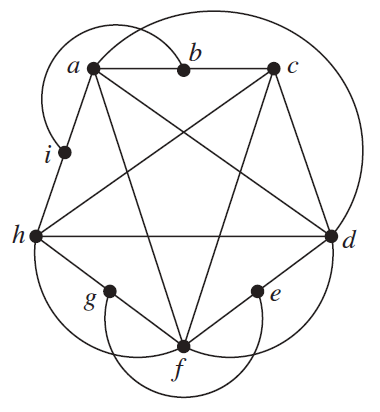
\includegraphics[width=0.3\textwidth]{fig_10.7_24.png}
\end{center}

\textbf{解答：} 寻找同胚于 $K_5$ 的子图。

选取 5 个核心顶点：
\[ V = \{a, c, d, f, h\} \]

验证 $V$ 中任意两点间均存在内部顶点不相交的路径：
\begin{itemize}
    \item \textbf{内部 5 条弦（星形边）：} $(a,d), (a,f), (c,f), (c,h), (d,h)$ 均为直接边。
    \item \textbf{外部 5 条路径（沿外圈）：}
    \begin{itemize}
        \item $a$ 到 $c$：路径 $a \to b \to c$（中间顶点 $b$）。
        \item $c$ 到 $d$：直接边 $(c,d)$。
        \item $d$ 到 $f$：路径 $d \to e \to f$（中间顶点 $e$）。
        \item $f$ 到 $h$：路径 $f \to g \to h$（中间顶点 $g$）。
        \item $h$ 到 $a$：路径 $h \to i \to a$（中间顶点 $i$）。
    \end{itemize}
\end{itemize}

中间顶点 $b,e,g,i$ 互不相同，且均不属于核心集合 $V$。因此，这 5 个顶点及上述 10 条内部不相交路径构成了一个同胚于 $K_5$ 的子图。

\textbf{结论：} 根据库拉托夫斯基定理，该图\textbf{不是平面图}。

\newpage

\section{第10章（续）：最短路径算法}

本节讨论带权图中单源最短路径（Dijkstra 算法）与全源最短路径（Floyd-Warshall 算法）的原理、步骤与正确性证明。

\subsection{10.6 最短路径问题 (Section 10.6)}

\subsubsection*{概念补充}
\begin{itemize}
    \item \textbf{Dijkstra 算法：} 求解非负权图中单源最短路径。维护已确定最短距离的顶点集 $S$，每次从 $V \setminus S$ 中选择当前距离标号最小的顶点加入 $S$，并松弛其所有出边。
    \item \textbf{Floyd-Warshall 算法：} 求解任意两点间最短路径，允许负权边但不可有负权回路。通过动态规划逐步允许顶点 $v_k$ 作为中间点：
    \[ d_{ij}^{(k)} = \min\!\left(d_{ij}^{(k-1)},\ d_{ik}^{(k-1)} + d_{kj}^{(k-1)}\right) \]
    \item \textbf{前驱记录：} 扩展 Dijkstra 时维护 $\text{previous}[v]$，可在算法结束后通过回溯构造具体最短路径。
\end{itemize}

\subsubsection*{习题 10.6-2}
\textbf{题目：} 使用 Dijkstra 算法求图中顶点 $a$ 到 $z$ 之间的最短路径长度。

\begin{center}
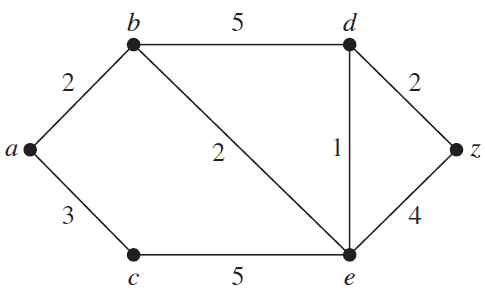
\includegraphics[width=0.3\textwidth]{fig_10.6_2.png}
\end{center}

\textbf{已知权重：} $w(a,b)=2,\ w(a,c)=3,\ w(b,d)=5,\ w(b,e)=2,\ w(c,e)=5,\ w(d,e)=1,\ w(d,z)=2,\ w(e,z)=4$。

\textbf{解答：} 逐步执行 Dijkstra 算法，集合 $S$ 为已确定最短距离的顶点集。

\begin{center}
\begin{tabular}{c|c|l}
步骤 & 加入 $S$ 的顶点 & 距离标号更新（仅列出变化项） \\
\hline
初始 & --- & $L(a)=0$；其余 $L(v)=\infty$ \\
1 & $a$ & $L(b)=2,\ L(c)=3$ \\
2 & $b$ ($L=2$) & $L(d)=7,\ L(e)=4$ \\
3 & $c$ ($L=3$) & $L(e)=\min(4,3+5)=4$（不变） \\
4 & $e$ ($L=4$) & $L(d)=\min(7,4+1)=5,\ L(z)=8$ \\
5 & $d$ ($L=5$) & $L(z)=\min(8,5+2)=7$ \\
6 & $z$ ($L=7$) & 算法终止
\end{tabular}
\end{center}

\textbf{最短路径长度：} $\mathbf{7}$。\\
\textbf{最短路径：} $\mathbf{a \to b \to e \to d \to z}$。

\subsubsection*{习题 10.6-21（完整精确解答）}
\textbf{题目：} 使用 Floyd 算法找出图 4(a) 中所有顶点对之间的最短距离。

\begin{center}
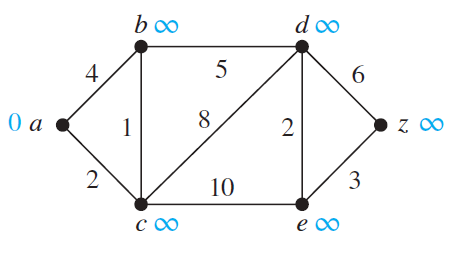
\includegraphics[width=0.5\textwidth]{fig_10.6_21.png}
\end{center}

\textbf{已知边权重（顶点顺序 $a,b,c,d,e,z$）：}
\[
\begin{aligned}
&w(a,b)=4,\ w(a,c)=2 \\
&w(b,c)=1,\ w(b,d)=5 \\
&w(c,d)=8,\ w(c,e)=10 \\
&w(d,e)=2,\ w(d,z)=6 \\
&w(e,z)=3
\end{aligned}
\]

\textbf{Floyd-Warshall 完整迭代过程：}

\textbf{步骤 0 — 初始矩阵 $D^{(0)}$：}

\[
D^{(0)} = \begin{bmatrix}
0 & 4 & 2 & \infty & \infty & \infty \\
4 & 0 & 1 & 5 & \infty & \infty \\
2 & 1 & 0 & 8 & 10 & \infty \\
\infty & 5 & 8 & 0 & 2 & 6 \\
\infty & \infty & 10 & 2 & 0 & 3 \\
\infty & \infty & \infty & 6 & 3 & 0
\end{bmatrix}
\]

\textbf{步骤 1 — 允许 $a$ 作为中间点（$k=a$）：}
检查所有 $d_{ij} = \min(d_{ij}, d_{ia}+d_{aj})$。由于 $d_{xa}=\infty$（$x=d,e,z$），仅涉及 $a$ 的行/列无改进。
\[
D^{(1)} = D^{(0)}
\]

\textbf{步骤 2 — 允许 $b$ 作为中间点（$k=b$）：}
\begin{itemize}
    \item $d_{ad} = \min(\infty, 4+5) = 9$
    \item $d_{cd} = \min(8, 1+5) = 6$
    \item $d_{da} = \min(\infty, 5+4) = 9$
    \item $d_{dc} = \min(8, 5+1) = 6$
\end{itemize}

\[
D^{(2)} = \begin{bmatrix}
0 & 4 & 2 & 9 & \infty & \infty \\
4 & 0 & 1 & 5 & \infty & \infty \\
2 & 1 & 0 & 6 & 10 & \infty \\
9 & 5 & 6 & 0 & 2 & 6 \\
\infty & \infty & 10 & 2 & 0 & 3 \\
\infty & \infty & \infty & 6 & 3 & 0
\end{bmatrix}
\]

\textbf{步骤 3 — 允许 $c$ 作为中间点（$k=c$）：}
\begin{itemize}
    \item $d_{ad} = \min(9, 2+6) = 8$
    \item $d_{ae} = \min(\infty, 2+10) = 12$
    \item $d_{be} = \min(\infty, 1+10) = 11$
    \item $d_{da} = \min(9, 6+2) = 8$
    \item $d_{ea} = \min(\infty, 10+2) = 12$
    \item $d_{eb} = \min(\infty, 10+1) = 11$
\end{itemize}

\[
D^{(3)} = \begin{bmatrix}
0 & 4 & 2 & 8 & 12 & \infty \\
4 & 0 & 1 & 5 & 11 & \infty \\
2 & 1 & 0 & 6 & 10 & \infty \\
8 & 5 & 6 & 0 & 2 & 6 \\
12 & 11 & 10 & 2 & 0 & 3 \\
\infty & \infty & \infty & 6 & 3 & 0
\end{bmatrix}
\]

\textbf{步骤 4 — 允许 $d$ 作为中间点（$k=d$）：}
\begin{itemize}
    \item $d_{ae} = \min(12, 8+2) = 10$
    \item $d_{az} = \min(\infty, 8+6) = 14$
    \item $d_{be} = \min(11, 5+2) = 7$
    \item $d_{bz} = \min(\infty, 5+6) = 11$
    \item $d_{ce} = \min(10, 6+2) = 8$
    \item $d_{cz} = \min(\infty, 6+6) = 12$
    \item $d_{ea} = \min(12, 2+8) = 10$
    \item $d_{eb} = \min(11, 2+5) = 7$
    \item $d_{ec} = \min(10, 2+6) = 8$
    \item $d_{za} = \min(\infty, 6+8) = 14$
    \item $d_{zb} = \min(\infty, 6+5) = 11$
    \item $d_{zc} = \min(\infty, 6+6) = 12$
\end{itemize}

\[
D^{(4)} = \begin{bmatrix}
0 & 4 & 2 & 8 & 10 & 14 \\
4 & 0 & 1 & 5 & 7 & 11 \\
2 & 1 & 0 & 6 & 8 & 12 \\
8 & 5 & 6 & 0 & 2 & 6 \\
10 & 7 & 8 & 2 & 0 & 3 \\
14 & 11 & 12 & 6 & 3 & 0
\end{bmatrix}
\]

\textbf{步骤 5 — 允许 $e$ 作为中间点（$k=e$）：}
\begin{itemize}
    \item $d_{az} = \min(14, 10+3) = 13$
    \item $d_{bz} = \min(11, 7+3) = 10$
    \item $d_{cz} = \min(12, 8+3) = 11$
    \item $d_{dz} = \min(6, 2+3) = 5$
    \item $d_{za} = \min(14, 3+10) = 13$
    \item $d_{zb} = \min(11, 3+7) = 10$
    \item $d_{zc} = \min(12, 3+8) = 11$
    \item $d_{zd} = \min(6, 3+2) = 5$
\end{itemize}

\[
D^{(5)} = \begin{bmatrix}
0 & 4 & 2 & 8 & 10 & 13 \\
4 & 0 & 1 & 5 & 7 & 10 \\
2 & 1 & 0 & 6 & 8 & 11 \\
8 & 5 & 6 & 0 & 2 & 5 \\
10 & 7 & 8 & 2 & 0 & 3 \\
13 & 10 & 11 & 5 & 3 & 0
\end{bmatrix}
\]

\textbf{步骤 6 — 允许 $z$ 作为中间点（$k=z$）：}
通过 $z$ 的路径均更长，无改进。

\textbf{最终矩阵 $D^{(6)}$：}

\[
\mathbf{D^{(6)} = \begin{bmatrix}
0 & 4 & 2 & 8 & 10 & 13 \\
4 & 0 & 1 & 5 & 7 & 10 \\
2 & 1 & 0 & 6 & 8 & 11 \\
8 & 5 & 6 & 0 & 2 & 5 \\
10 & 7 & 8 & 2 & 0 & 3 \\
13 & 10 & 11 & 5 & 3 & 0
\end{bmatrix}}
\]

\textbf{全源最短距离表（行 $\to$ 列）：}

\begin{center}
\begin{tabular}{c|cccccc}
 & $a$ & $b$ & $c$ & $d$ & $e$ & $z$ \\
\hline
$a$ & 0 & 4 & 2 & 8 & 10 & $\mathbf{13}$ \\
$b$ & 4 & 0 & 1 & 5 & 7 & $\mathbf{10}$ \\
$c$ & 2 & 1 & 0 & 6 & 8 & $\mathbf{11}$ \\
$d$ & 8 & 5 & 6 & 0 & 2 & $\mathbf{5}$ \\
$e$ & 10 & 7 & 8 & 2 & 0 & $\mathbf{3}$ \\
$z$ & 13 & 10 & 11 & 5 & 3 & 0
\end{tabular}
\end{center}

\textbf{关键最短路径及路径还原：}
\begin{itemize}
    \item $a \to z$: 距离 $\mathbf{13}$，路径 $a \to c \to b \to d \to e \to z$（$2+1+5+2+3=13$）
    \item $b \to z$: 距离 $\mathbf{10}$，路径 $b \to d \to e \to z$（$5+2+3=10$）
    \item $c \to z$: 距离 $\mathbf{11}$，路径 $c \to b \to d \to e \to z$（$1+5+2+3=11$）
    \item $d \to z$: 距离 $\mathbf{5}$，路径 $d \to e \to z$（$2+3=5$）
    \item $a \to e$: 距离 $\mathbf{10}$，路径 $a \to c \to b \to d \to e$（$2+1+5+2=10$）
    \item $a \to d$: 距离 $\mathbf{8}$，路径 $a \to c \to b \to d$（$2+1+5=8$）
    \item $e \to a$: 距离 $\mathbf{10}$，路径 $e \to d \to c \to a$（$2+6+2=10$）
    \item $z \to a$: 距离 $\mathbf{13}$，路径 $z \to e \to d \to c \to a$（$3+2+6+2=13$）
\end{itemize}

\subsubsection*{补充题 1：扩展 Dijkstra 算法（路径构造）}
\textbf{题目：} 扩展加权简单连通图上的 Dijkstra 算法，使其不仅能求出最短距离，还能构造出从 $v_0$ 到所有顶点的最短路径。

\textbf{解答：} 引入前驱数组 $\text{previous}[v]$ 记录最短路径上 $v$ 的前一个顶点。

\begin{verbatim}
procedure extended_dijkstra(G: weighted connected simple graph)
    {顶点集 V = {v_0, v_1, ..., v_n}，权重 w(u,v) > 0}
    for each v $\in$ V
        L(v) := ∞
        previous(v) := undefined
    L(v_0) := 0
    S := $\emptyset$  {已确定最短路径的顶点集}
    
    while V \ S $\neq$ $\emptyset$
        u := V \ S 中 L(u) 最小的顶点
        S := S $\cup$ {u}
        for each v $\in$ V \ S adjacent to u
            if L(u) + w(u,v) < L(v) then
                L(v) := L(u) + w(u,v)
                previous(v) := u
    
    {构造到顶点 v 的具体路径}
    procedure get_path(v)
        path := [v]
        while previous(v) is defined
            v := previous(v)
            prepend v to path
        return path
\end{verbatim}

\textbf{复杂度：} 与标准 Dijkstra 相同，为 $O(|V|^2)$（数组实现）或 $O(|E| + |V|\log|V|)$（优先队列实现）。

\subsubsection*{补充题 2：Floyd-Warshall 算法正确性证明}
\textbf{题目：} 证明加权简单有向图（边权可为负，但无负权回路）上 Floyd-Warshall 算法的正确性。

\textbf{证明：} 对中间顶点集合的规模 $k$ 使用数学归纳法。

\begin{enumerate}[1.]
    \item \textbf{基础步 ($k=0$)：} $D^{(0)}$ 仅允许直接边，$d_{ij}^{(0)}$ 为 $(v_i,v_j)$ 的权重或 $\infty$。显然正确。
    
    \item \textbf{归纳步：} 假设 $D^{(k-1)}$ 已正确记录限制中间顶点在 $\{v_1,\dots,v_{k-1}\}$ 内的最短距离。考虑加入 $v_k$ 作为新的允许中间点。
    
    对任意顶点对 $(v_i,v_j)$，设 $P$ 为限制中间顶点在 $\{v_1,\dots,v_k\}$ 内的最短路径，则：
    \begin{itemize}
        \item \textbf{情况 1：} $v_k$ 不在 $P$ 上。则 $P$ 的中间顶点仍在 $\{v_1,\dots,v_{k-1}\}$ 内，故 $d_{ij}^{(k)} = d_{ij}^{(k-1)}$。
        \item \textbf{情况 2：} $v_k$ 在 $P$ 上。因无负权回路，$v_k$ 在 $P$ 上仅出现一次。将 $P$ 拆分为 $v_i \leadsto v_k$ 与 $v_k \leadsto v_j$ 两段，两段中间顶点均取自 $\{v_1,\dots,v_{k-1}\}$。由归纳假设，其长度分别为 $d_{ik}^{(k-1)}$ 与 $d_{kj}^{(k-1)}$，故
        \[ d_{ij}^{(k)} = d_{ik}^{(k-1)} + d_{kj}^{(k-1)} \]
    \end{itemize}
    算法取两者最小值，状态转移方程
    \[ d_{ij}^{(k)} = \min\!\left(d_{ij}^{(k-1)},\ d_{ik}^{(k-1)} + d_{kj}^{(k-1)}\right) \]
    恰好覆盖了上述两种最优情况。
    
    \item \textbf{结论：} 当 $k=n$ 时，所有顶点均可作为中间点，$D^{(n)}$ 给出真正的全源最短距离。证毕。
\end{enumerate}

\newpage

\section{第11章：树}

树是连通无回路的简单图，在计算机科学中具有广泛的建模与应用价值。本章介绍树的基本刻画定理及其在决策与搜索中的应用。

\subsection{11.1 树的介绍 (Section 11.1)}

\subsubsection*{概念补充}
\begin{itemize}
    \item \textbf{树 (Tree)：} 连通且无简单回路的简单图。
    \item \textbf{等价刻画：} 对于 $n$ 个顶点的简单图，以下三者等价：
    \begin{enumerate}[(1)]
        \item $G$ 是树；
        \item $G$ 连通且有 $n-1$ 条边；
        \item $G$ 无回路且有 $n-1$ 条边。
    \end{enumerate}
    \item \textbf{森林 (Forest)：} 无回路的简单图（若干棵树的并）。
    \item \textbf{满 $m$ 叉树 (Full $m$-ary Tree)：} 每个内点恰好有 $m$ 个子节点。满足 $l = (m-1)i + 1$，其中 $l$ 为叶子数，$i$ 为内点数。
\end{itemize}

\subsubsection*{习题 11.1-14}
\textbf{题目：} 证明一个简单图是树，当且仅当它是连通的，但删除其中任意一条边都会产生一个不连通的图。

\textbf{证明：}

\textbf{($\Rightarrow$)} 设 $G$ 是树。由定义，$G$ 连通且无回路。对任意边 $e=\{u,v\} \in E$，由于树中任意两点间有且仅有一条简单路径，$e$ 就是 $u$ 与 $v$ 之间的唯一路径。删除 $e$ 后 $u$ 与 $v$ 不再连通，故 $G-e$ 不连通。

\textbf{($\Leftarrow$)} 设 $G$ 连通，且删去任意边均导致不连通。假设 $G$ 含简单回路 $C$，取 $C$ 上的一条边 $e$。因 $e$ 位于回路上，其两端点在 $G-e$ 中仍可通过回路的剩余部分相连，故 $G-e$ 仍连通，与条件矛盾。因此 $G$ 无回路，结合连通性可知 $G$ 是树。

\subsubsection*{习题 11.1-15}
\textbf{题目：} 令 $G$ 是有 $n$ 个顶点的简单图。证明：\\
\textbf{a)} $G$ 是树 $\iff$ $G$ 连通且有 $n-1$ 条边。\\
\textbf{b)} $G$ 是树 $\iff$ $G$ 无简单回路且有 $n-1$ 条边。

\textbf{证明：}

\textbf{a)} 
\begin{itemize}
    \item \textbf{($\Rightarrow$)} 对 $n$ 归纳。$n=1$ 时显然。假设 $n$ 个顶点的树有 $n-1$ 条边。对 $n+1$ 个顶点的树，删去任一片叶子（度数为 1 的顶点必存在），得到 $n$ 顶点树，有 $n-1$ 条边；还原叶子后增加 1 条边，共 $n$ 条边。
    \item \textbf{($\Leftarrow$)} 设 $G$ 连通且有 $n-1$ 条边。若 $G$ 不是树，则 $G$ 含回路。不断删去回路上的边直至无回路，得到一棵生成树 $T$。$T$ 有 $n-1$ 条边，与 $G$ 原有边数相同，说明未删去任何边，即 $G$ 本身无回路，是树。
\end{itemize}

\textbf{b)}
\begin{itemize}
    \item \textbf{($\Rightarrow$)} 若 $G$ 是树，由定义无回路，由 \textbf{a)} 有 $n-1$ 条边。
    \item \textbf{($\Leftarrow$)} 设 $G$ 无回路且有 $n-1$ 条边。设 $G$ 有 $k$ 个连通分支 $C_1,\dots,C_k$，各分支均为树。设 $C_j$ 有 $n_j$ 个顶点，则边数为 $n_j-1$。总边数
    \[ |E| = \sum_{j=1}^k (n_j-1) = \left(\sum_{j=1}^k n_j\right) - k = n - k \]
    已知 $|E| = n-1$，故 $n-k = n-1 \Rightarrow k=1$。即 $G$ 只有一个连通分支，故 $G$ 连通。结合无回路，$G$ 是树。
\end{itemize}

\subsubsection*{习题 11.1-24}
\textbf{题目：} 要么画出一棵叶子数为 $76$、高度为 $3$ 的满 $m$ 叉树（其中 $m$ 为正整数），要么证明这样的树不存在。

\textbf{解答：}

满 $m$ 叉树满足 $l = (m-1)i + 1$，其中 $l$ 为叶子数，$i$ 为内点数。代入 $l=76$：
\[ 76 = (m-1)i + 1 \implies 75 = (m-1)i \]

取 $m-1=5$（即 $m=6$），则 $i=15$。总顶点数 $n = mi + 1 = 91$。

\textbf{构造验证（高度 $h=3$）：}
\begin{itemize}
    \item 第 $0$ 层（根）：$1$ 个内点。
    \item 第 $1$ 层：$6$ 个节点。令其中 $2$ 个为内点，$4$ 个为叶子。
    \item 第 $2$ 层：$2 \times 6 = 12$ 个节点。令全部 $12$ 个为内点。
    \item 第 $3$ 层：$12 \times 6 = 72$ 个叶子。
\end{itemize}
总内点数：$1 + 2 + 12 = 15$。总叶子数：$4 + 72 = 76$。最长路径恰为 $3$，满足高度要求。

\textbf{结论：} 这样的树\textbf{存在}。例如 $m=6$ 时，其结构示意如下：

\begin{center}
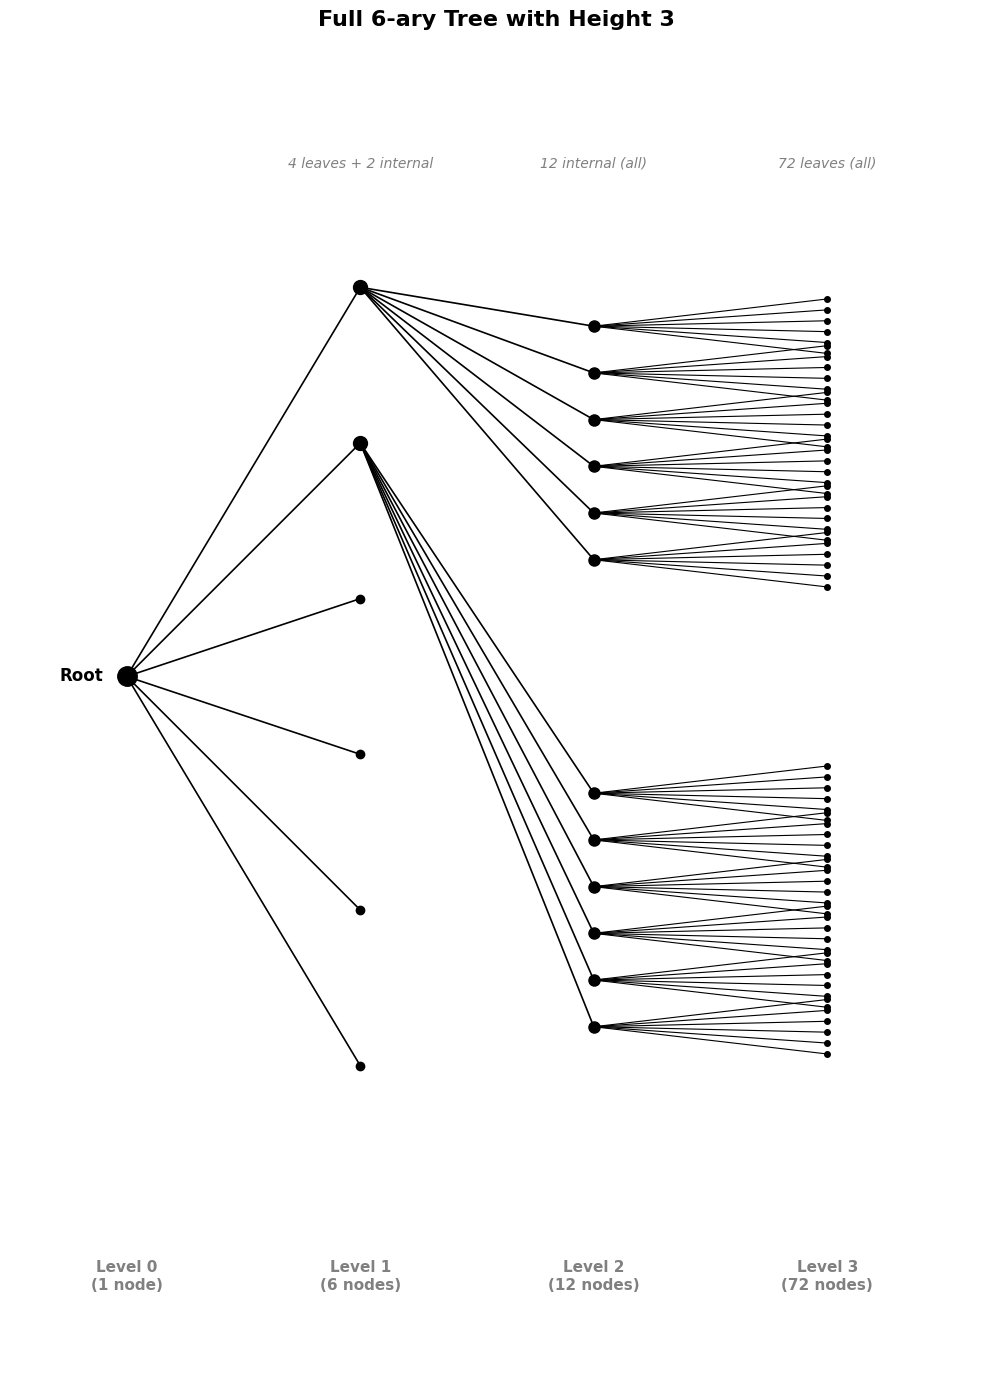
\includegraphics[width=0.65\textwidth]{fig_11.1_24.png}
\end{center}

\subsection{11.2 树的应用 (Section 11.2)}

\subsubsection*{概念补充}
\begin{itemize}
    \item \textbf{决策树 (Decision Tree)：} 用树形结构表示一系列决策过程，每个内点对应一次测试/比较，每个叶子对应一个最终结论。
    \item \textbf{信息论下界：} 若问题有 $N$ 种可能结果，每次测试有 $t$ 种结果，则决策树高度至少为 $\lceil \log_t N \rceil$。
\end{itemize}

\subsubsection*{习题 11.2-8}
\textbf{题目：} 在 $8$ 枚硬币中有一枚伪币，伪币可能比真币重也可能轻。至少需要称重几次才能找到这枚伪币？描述对应的算法。

\textbf{解答：}

\textbf{信息量分析：}
\begin{itemize}
    \item $8$ 枚硬币中每一枚都可能是伪币，且各有“重”或“轻”两种可能，共 $8 \times 2 = 16$ 种等可能情况。
    \item 每次天平称重有 $3$ 种结果：左重、右重、平衡。
    \item 决策树高度为 $h$ 时最多区分 $3^h$ 种情况。由 $3^2=9 < 16 \le 27=3^3$，得
    \[ \mathbf{h \ge 3} \]
    即\textbf{至少需要称重 3 次}。
\end{itemize}
\textbf{3 次称重算法（决策树描述）：}

将硬币编号为 $1,2,3,4,5,6,7,8$。

\begin{enumerate}[1.]
    \item \textbf{第一次称重：} 称 $\{1,2,3\}$ 对 $\{4,5,6\}$。
    \begin{itemize}
        \item \textbf{若平衡：} 伪币在 $\{7,8\}$ 中。第二次称 $7$ 对 $1$（真币）。若平衡则 $8$ 为伪币；否则 $7$ 为伪币。第三次称可确定轻重。
        \item \textbf{若左重（或左轻）：} 伪币在 $\{1,2,3,4,5,6\}$ 中，且已知 $7,8$ 为真币。此时不仅缩小了范围，还获得了“伪币在左侧则偏重、在右侧则偏轻”的关联信息。
    \end{itemize}
    
    \item \textbf{第二次称重（以第一次左重为例）：} 称 $\{1,2,4\}$ 对 $\{3,7,8\}$（利用已知真币 $7,8$）。
    \begin{itemize}
        \item 若平衡：伪币在 $\{5,6\}$ 中且偏轻（因第一次左重意味着伪币在右侧则轻）。第三次称 $5$ 对 $7$ 即可确定。
        \item 若左重：伪币在 $\{1,2\}$ 中且偏重；或伪币为 $4$ 且偏轻。第三次称 $1$ 对 $2$ 可区分。
        \item 若右重：伪币为 $3$ 且偏重，或伪币为 $4$ 且偏轻。第三次称 $3$ 对 $7$ 可区分。
    \end{itemize}
    
    \item \textbf{第三次称重：} 在前两次结果的基础上，将可疑硬币与已知真币比较，即可唯一确定伪币及其轻重。
\end{enumerate}

\textbf{结论：} 最少需要 $\mathbf{3}$ 次称重，且上述决策树覆盖了全部 $16$ 种情况。

\newpage
\section{第1章：命题逻辑}

\subsection{命题与逻辑联结词 (Section 1.1)}

\subsubsection*{习题 1.1-14}
\textbf{题目：} 令 $p, q, r$ 为以下命题：
\begin{itemize}
    \item $p$：You have the flu.
    \item $q$：You miss the final examination.
    \item $r$：You pass the course.
\end{itemize}
将下列各复合命题表示为英文句子。
\begin{enumerate}[a)]
    \item $p \to q$
    \item $\neg q \leftrightarrow r$
    \item $q \to \neg r$
    \item $p \lor q \lor r$
    \item $(p \to \neg r) \lor (q \to \neg r)$
    \item $(p \land q) \lor (\neg q \land r)$
\end{enumerate}

\textbf{解答：}
\begin{center}
\begin{tabular}{c|l|l}
\hline
命题 & 中文 & English \\
\hline
(a) $p \to q$ & 得流感则错过期末 & If you have the flu, then you miss the final examination. \\
(b) $\neg q \leftrightarrow r$ & 未错过期末当且仅当通过课程 & You do not miss the final examination iff you pass the course. \\
(c) $q \to \neg r$ & 错过期末则不能通过课程 & If you miss the final examination, then you do not pass the course. \\
(d) $p \lor q \lor r$ & 得流感、错过期末或通过课程 & You have the flu, or you miss the final examination, or you pass the course. \\
(e) $(p \to \neg r) \lor (q \to \neg r)$ & 要么（得流感则不能通过），要么（错过期末则不能通过） & Either (flu $\Rightarrow$ not pass) or (miss final $\Rightarrow$ not pass). \\
(f) $(p \land q) \lor (\neg q \land r)$ & 要么（流感且错过期末），要么（未错过期末且通过） & Either (flu and miss final) or (not miss final and pass). \\
\hline
\end{tabular}
\end{center}

\subsubsection*{习题 1.1-15}
\textbf{题目：} 令 $p$ 和 $q$ 为以下命题：
\begin{itemize}
    \item $p$：You drive over 65 miles per hour.
    \item $q$：You get a speeding ticket.
\end{itemize}
用 $p$、$q$ 及逻辑联结词（包括否定）写出下列各命题。
\begin{enumerate}[a)]
    \item You do not drive over 65 miles per hour.
    \item You drive over 65 miles per hour, but you do not get a speeding ticket.
    \item You will get a speeding ticket if you drive over 65 miles per hour.
    \item If you do not drive over 65 miles per hour, then you will not get a speeding ticket.
    \item Driving over 65 miles per hour is sufficient for getting a speeding ticket.
    \item You get a speeding ticket, but you do not drive over 65 miles per hour.
    \item Whenever you get a speeding ticket, you are driving over 65 miles per hour.
\end{enumerate}

\textbf{解答：}
\begin{center}
\begin{tabular}{c|c|l|l}
\hline
 & 符号 & English & 中文 \\
\hline
(a) & $\neg p$ & You do not drive over 65 mph. & 未超速 \\
(b) & $p \land \neg q$ & Over 65 mph but no ticket. & 超速且无罚单 \\
(c) & $p \to q$ & Ticket if over 65 mph. & 超速则罚单 \\
(d) & $\neg p \to \neg q$ & No over 65 mph $\to$ no ticket. & 未超速则无罚单 \\
(e) & $p \to q$ & Over 65 mph sufficient for ticket. & 超速是罚单充分条件 \\
(f) & $q \land \neg p$ & Ticket but not over 65 mph. & 有罚单但未超速 \\
(g) & $q \to p$ & Ticket $\Rightarrow$ over 65 mph. & 有罚单则超速 \\
\hline
\end{tabular}
\end{center}

\subsubsection*{习题 1.1-34}
\textbf{题目：} 为下列各复合命题构造真值表。
\begin{enumerate}[a)]
    \item $p \to \neg p$
    \item $p \leftrightarrow \neg p$
    \item $p \oplus (p \lor q)$
    \item $(p \land q) \to (p \lor q)$
\end{enumerate}

\textbf{解答：}
\begin{center}
\begin{tabular}{cc|cccc}
\hline
$p$ & $q$ & (a) & (b) & (c) & (d) \\
\hline
T & T & F & F & F & T \\
T & F & F & F & F & T \\
F & T & T & F & T & T \\
F & F & T & F & F & T \\
\hline
\end{tabular}
\end{center}
\begin{itemize}
    \item (a) 与 $p$ 相反（恒为 $\neg p$）；
    \item (b) 恒为 $\mathbf{F}$；
    \item (c) 仅当 $(p,q)=(F,T)$ 时为 $\mathbf{T}$；
    \item (d) 恒为 $\mathbf{T}$（重言式）。
\end{itemize}

\subsubsection*{习题 1.1-35}
\textbf{题目：} 为下列各复合命题构造真值表。
\begin{enumerate}[a)]
    \item $(p \lor q) \to (p \oplus q)$
    \item $(p \oplus q) \to (p \land q)$
    \item $(p \lor q) \oplus (p \land q)$
    \item $(p \leftrightarrow q) \oplus (\neg p \leftrightarrow q)$
\end{enumerate}

\textbf{解答：}
\begin{center}
\begin{tabular}{cc|cccc}
\hline
$p$ & $q$ & (a) & (b) & (c) & (d) \\
\hline
T & T & F & T & F & T \\
T & F & T & F & T & T \\
F & T & T & F & T & T \\
F & F & T & T & F & T \\
\hline
\end{tabular}
\end{center}
\begin{itemize}
    \item (a) 仅 $(T,T)$ 为 $\mathbf{F}$；
    \item (b) 恰有一真时为 $\mathbf{F}$；
    \item (c) 恰有一真时为 $\mathbf{T}$；
    \item (d) 恒为 $\mathbf{T}$（重言式）。
\end{itemize}



\subsection{命题等价与系统规范 (Section 1.2)}

\subsubsection*{习题 1.2-6}
\textbf{题目：} 你可以升级你的操作系统，当且仅当你拥有以下配置之一：
\begin{itemize}
    \item 32位处理器且主频不低于1 GHz、至少1 GB内存、至少16 GB空闲硬盘空间；或
    \item 64位处理器且主频不低于2 GHz、至少2 GB内存、至少32 GB空闲硬盘空间。
\end{itemize}
令 $u$：``You can upgrade your operating system,'' $b_{32}$：``You have a 32-bit processor,'' $b_{64}$：``You have a 64-bit processor,'' $g_1$：``Your processor runs at 1 GHz or faster,'' $g_2$：``Your processor runs at 2 GHz or faster,'' $r_1$：``Your processor has at least 1 GB RAM,'' $r_2$：``Your processor has at least 2 GB RAM,'' $h_{16}$：``You have at least 16 GB free hard disk space,'' $h_{32}$：``You have at least 32 GB free hard disk space.'' 用这些命题变量表达上述升级条件。

\textbf{解答：}
\[ u \to \Bigl((b_{32} \land g_1 \land r_1 \land h_{16}) \lor (b_{64} \land g_2 \land r_2 \land h_{32})\Bigr). \]

\subsubsection*{习题 1.2-10}
\textbf{题目：} 判断下列系统规范是否一致：``Whenever the system software is being upgraded, users cannot access the file system. If users can access the file system, then they can save new files. If users cannot save new files, then the system software is not being upgraded.''

\textbf{解答：}

\textbf{符号化：} 令 $p$：系统正在升级；$q$：用户可以访问文件系统；$r$：用户可以保存新文件。
\begin{enumerate}
    \item Whenever upgraded $\Rightarrow$ no access：$p \to \neg q$
    \item Access $\Rightarrow$ save：$q \to r$
    \item Cannot save $\Rightarrow$ not upgrading：$\neg r \to \neg p\ (\equiv p \to r)$
\end{enumerate}

\textbf{相容性判断：} 将三式化为合取范式（CNF）：
\[ (\neg p \lor \neg q) \land (\neg q \lor r) \land (\neg p \lor r). \]
取赋值 $(p,q,r) = (F,F,F)$，各子句均为真，故\textbf{系统规范是相容的}。

\subsubsection*{习题 1.2-34}
\textbf{题目：} （习题 28--35 共同背景）一座岛上有三种居民：骑士（knights），他们总是说真话；无赖（knaves），他们总是说谎；间谍（spies，Smullyan 称之为 normals），他们有时说真话有时说谎。你遇到三个人 $A, B, C$。已知他们中恰好有一个骑士、一个无赖、一个间谍。每个人都清楚另外两人的身份。对下列情形，判断是否存在唯一解，并确定谁是骑士、无赖和间谍；若无唯一解，列出所有可能解或说明无解。

\textbf{具体情形：} $A$ 说 ``I am not the spy,'' $B$ 说 ``I am not the spy,'' $C$ 说 ``$A$ is the spy.''

\textbf{解答：} 设 $S_A, S_B, S_C$ 分别表示 $A, B, C$ 为间谍。
\begin{itemize}
    \item \textbf{若 $C$ 为骑士：} 则 $S_A$ 为真，即 $A$ 是间谍；那么 $B$ 必为无赖。但 $B$ 说 ``I am not the spy''，若 $B$ 是无赖，则此话应为假，即 $B$ 是间谍，与 $A$ 是间谍矛盾（ spy 唯一）。
    \item \textbf{若 $C$ 为无赖：} 则 $S_A$ 为假，$A$ 不是间谍。此时若 $B$ 为间谍，则 $A$ 必为骑士。验证：$A$（骑士）说 ``I am not the spy'' 为真；$B$（间谍）说 ``I am not the spy'' 可真可假；$C$（无赖）说 ``$A$ is the spy'' 为假（因 $A$ 是骑士）。此分配\textbf{一致}。
    \item \textbf{若 $C$ 为间谍：} 则 $A, B$ 中一为骑士一为无赖。$B$ 说 ``I am not the spy''，若 $B$ 为无赖则此话为假，即 $B$ 是间谍，与 $C$ 是间谍矛盾；若 $B$ 为骑士则此话为真，但 $A$ 必为无赖，$A$ 说 ``I am not the spy'' 为假，即 $A$ 是间谍，与 $C$ 是间谍矛盾。
\end{itemize}
\textbf{结论：} 存在唯一解：$\mathbf{A=Knight,\ B=Spy,\ C=Knave}$。

\subsubsection*{习题 1.2-40}
\textbf{题目：} 四位朋友 Alice、John、Carlos、Diana 被认定为一起非法入侵计算机系统案件的嫌疑人。他们分别向调查人员作出如下陈述：
\begin{itemize}
    \item Alice：``Carlos did it.''
    \item John：``I did not do it.''
    \item Carlos：``Diana did it.''
    \item Diana：``Carlos lied when he said that I did it.''
\end{itemize}
\begin{enumerate}[a)]
    \item 若调查人员还知道四人中恰好只有一人说真话，是谁做的？说明理由。
    \item 若调查人员还知道四人中恰好只有一人说谎，是谁做的？说明理由。
\end{enumerate}

\textbf{解答（仅 b 部分）：}

\textbf{证法一（固定作案者）：} 设作案者为 $A, J, C, D$ 中恰一人。各陈述内容分别为 $S_A=C$（Carlos作案）、$S_J=\neg J$（John没做）、$S_C=D$（Diana作案）、$S_D=\neg D$（Carlos说谎，即Diana没做）。
\begin{center}
\begin{tabular}{c|cccc|c}
\hline
假设作案者 & $S_A=C$ & $S_J=\neg J$ & $S_C=D$ & $S_D=\neg D$ & 说谎数 \\
\hline
Alice   & 假 & 真 & 假 & 真 & 2 \\
John    & 假 & 假 & 假 & 真 & 3 \\
Carlos  & 真 & 真 & 假 & 假 & \textbf{1} \\
Diana   & 假 & 真 & 真 & 假 & 2 \\
\hline
\end{tabular}
\end{center}
仅当作案者为 Carlos 时，恰有 1 人说谎（Carlos 自己）。

\textbf{证法二（设唯一说谎者）：}
\begin{itemize}
    \item \textbf{假设 Alice 说谎：} 则 $C$ 假（Carlos没做），且其余三人真话。John 真 $\Rightarrow J$ 没做；Carlos 真 $\Rightarrow D$ 做；Diana 真 $\Rightarrow \neg D$（Diana没做）。$D$ 与 $\neg D$ 矛盾。
    \item \textbf{假设 John 说谎：} 则 $J$ 真（John做了），且其余三人真话。Alice 真 $\Rightarrow C$ 做；Carlos 真 $\Rightarrow D$ 做。出现 $J, C, D$ 多人作案，与恰一人作案矛盾。
    \item \textbf{假设 Carlos 说谎：} 则 $D$ 假（Diana没做），且其余三人真话。Alice 真 $\Rightarrow C$ 做；John 真 $\Rightarrow J$ 没做；Diana 真 $\Rightarrow \neg D$。与恰一人作案相容（Carlos 作案）。
    \item \textbf{假设 Diana 说谎：} 则 $\neg D$ 假（即 $D$ 真），且其余三人真话。Alice 真 $\Rightarrow C$ 做；Carlos 真 $\Rightarrow D$ 做。$C, D$ 同作案，矛盾。
\end{itemize}
\textbf{结论：} 作案者是 $\mathbf{Carlos}$。



\subsection{命题等价与逻辑定律 (Section 1.3)}

\subsubsection*{习题 1.3-26}
\textbf{题目：} 证明 $(p \to q) \land (p \to r)$ 与 $p \to (q \land r)$ 逻辑等价。

\textbf{解答：}
\begin{align*}
(p \to q) \land (p \to r)
&\equiv (\neg p \lor q) \land (\neg p \lor r) \\
&\equiv \neg p \lor (q \land r) \qquad (\text{分配律}) \\
&\equiv p \to (q \land r).
\end{align*}

\subsubsection*{习题 1.3-32}
\textbf{题目：} 证明 $p \leftrightarrow q$ 与 $\neg p \leftrightarrow \neg q$ 逻辑等价。

\textbf{解答：}
\begin{align*}
p \leftrightarrow q &\equiv (\neg p \lor q) \land (\neg q \lor p), \\
\neg p \leftrightarrow \neg q &\equiv (p \lor \neg q) \land (q \lor \neg p).
\end{align*}
两式的子句完全相同，故逻辑等价。

\subsubsection*{附加题（DNF转换）}
\textbf{题目：} 将下列复合命题转化为析取范式（DNF）：
\[ (p \leftrightarrow \neg q) \land (q \leftrightarrow \neg r) \land \bigl(r \leftrightarrow (\neg p \land \neg q)\bigr) \]

\textbf{解答：}

\textbf{结构推理：} 由前两式可知 $p \equiv \neg r$ 且 $q \equiv \neg r$，故 $p \equiv q \equiv \neg r$。代入第三式：
\[ r \leftrightarrow (\neg r \land \neg q) \equiv r \leftrightarrow (\neg r \land r) \equiv r \leftrightarrow \mathbf{F} \equiv \neg r. \]
因此 $r$ 必为假，$p, q$ 必为真。唯一成真赋值为 $(p,q,r) = (F,T,F)$。

\textbf{真值表验证：} 仅 $(F,T,F)$ 使该复合命题为真。

\textbf{析取范式：} 直接写出唯一成真赋值对应的极小项：
\[ \mathbf{DNF} = \neg p \land q \land \neg r. \]

\subsubsection*{教材 Example 10（$n$ 皇后问题的可满足性建模）}
\textbf{题目：} 将 $n$ 皇后问题建模为可满足性问题。

$n$ 皇后问题要求在 $n \times n$ 棋盘上放置 $n$ 个皇后，使得任意两个皇后互不攻击（即不在同一行、同一列或同一对角线上）。为此引入 $n^2$ 个布尔变量 $p(i,j)$（$i,j = 1,2,\dots,n$），其中 $p(i,j)$ 为真当且仅当第 $i$ 行第 $j$ 列的方格上放置了皇后。

注意，方格 $(i,j)$ 与 $(i',j')$ 位于同一条对角线上，当且仅当 $i+i' = j+j'$ 或 $i-i' = j-j'$。

通过以下五个复合命题分别刻画约束：

\begin{enumerate}
    \item \textbf{每行至少一个皇后：}
    \[ Q_1 = \bigwedge_{i=1}^{n} \bigvee_{j=1}^{n} p(i,j) \]
    
    \item \textbf{每行至多一个皇后：} 对任意 $1 \le j < k \le n$，
    \[ Q_2 = \bigwedge_{i=1}^{n} \bigwedge_{j=1}^{n-1} \bigwedge_{k=j+1}^{n} \bigl(\neg p(i,j) \lor \neg p(i,k)\bigr) \]
    
    \item \textbf{每列至多一个皇后：} 对任意 $1 \le i < k \le n$，
    \[ Q_3 = \bigwedge_{j=1}^{n} \bigwedge_{i=1}^{n-1} \bigwedge_{k=i+1}^{n} \bigl(\neg p(i,j) \lor \neg p(k,j)\bigr) \]
    （此断言与 $Q_1$ 共同保证每列恰好有一个皇后。）
    
    \item \textbf{主对角线方向（左上至右下）上至多一个皇后：}
    \[ Q_4 = \bigwedge_{i=2}^{n} \bigwedge_{j=1}^{n-1} \bigwedge_{k=1}^{\min(i-1,n-j)} \bigl(\neg p(i,j) \lor \neg p(i-k,j+k)\bigr) \]
    
    \item \textbf{副对角线方向（右上至左下）上至多一个皇后：}
    \[ Q_5 = \bigwedge_{i=1}^{n-1} \bigwedge_{j=1}^{n-1} \bigwedge_{k=1}^{\min(n-i,n-j)} \bigl(\neg p(i,j) \lor \neg p(i+k,j+k)\bigr) \]
\end{enumerate}

最终，$n$ 皇后问题的所有解对应于使下列复合命题为真的变量赋值：
\[ Q = Q_1 \land Q_2 \land Q_3 \land Q_4 \land Q_5 \]

\subsubsection*{习题 1.3-68}
\textbf{题目：} 以习题 67（即 Example 10）中构造的复合命题 $Q$ 为起点，构造一个新的复合命题，使其能够找出 $n$ 皇后问题的所有满足如下条件的解：第一列中的皇后必须位于奇数编号的行上。

\textbf{解答：} 引入额外约束
\[ Q_6 = \bigvee_{\substack{1 \le i \le n \\ i \text{ 为奇数}}} p(i,1), \]
即第一列的皇后必须位于第 $1, 3, 5, \dots$ 等奇数行。将 $Q_6$ 与原有约束合取：
\[ Q' = Q_1 \land Q_2 \land Q_3 \land Q_4 \land Q_5 \land Q_6. \]
$Q'$ 的可满足赋值即对应第一列皇后在奇数行的全部 $n$ 皇后解。



\subsection{谓词与量词 (Section 1.4)}

\subsubsection*{概念补充：谓词翻译要点}
\textbf{注意：} 谓词翻译时应为每个符号写明在设定论域中的解释；$\forall, \exists$ 的语义依赖论域。请勿写非标准的 $\forall x \in S$ 形式，而应使用谓词限制，例如论域为全体学生时，应写
\[ \forall x \bigl(Student(x) \to Smart(x)\bigr), \]
而非 $\forall x \in Student,\ Smart(x)$（后者虽常见但非标准一阶逻辑写法）。

\subsubsection*{习题 1.4-42}
\textbf{题目：} 使用谓词、量词和逻辑联结词表达下列系统规范。
\begin{enumerate}[a)]
    \item 当硬盘剩余空间不足 30 兆字节时，向所有用户发送警告消息。
    \item 当检测到系统错误时，文件系统中的任何目录都无法打开，且任何文件都无法关闭。
    \item 如果当前有用户登录，则文件系统无法备份。
    \item 当可用内存至少为 8 兆字节且连接速度至少为 56 千比特每秒时，可以提供视频点播服务。
\end{enumerate}

\textbf{解答：}

\textbf{a)} 设论域为所有系统实体。定义谓词：
\begin{itemize}
    \item $s$：硬盘剩余空间不足 30 MB（0-ary 命题，或理解为 $Space(x)$ 的简写）；
    \item $U(x)$：$x$ 是用户；
    \item $W(x)$：已向 $x$ 发送警告消息。
\end{itemize}
则规范表示为：
\[ (s < 30) \to \forall x \bigl(U(x) \to W(x)\bigr). \]

\textbf{b)} 定义谓词：
\begin{itemize}
    \item $E$：检测到系统错误；
    \item $Dir(x)$：$x$ 是目录；
    \item $Open(x)$：目录 $x$ 可以打开；
    \item $File(y)$：$y$ 是文件；
    \item $Close(y)$：文件 $y$ 可以关闭。
\end{itemize}
则规范表示为：
\[ E \to \Bigl(\forall x \bigl(Dir(x) \to \neg Open(x)\bigr) \land \forall y \bigl(File(y) \to \neg Close(y)\bigr)\Bigr). \]

\textbf{c)} 定义谓词：
\begin{itemize}
    \item $L(x)$：$x$ 已登录；
    \item $B$：文件系统可以备份。
\end{itemize}
``有用户登录''即 $\exists x\, L(x)$，故规范表示为：
\[ (\exists x\, L(x)) \to \neg B. \]

\textbf{d)} 将系统状态视为 0-ary 命题变量：
\begin{itemize}
    \item $M$：可用内存至少为 8 MB；
    \item $S$：连接速度至少为 56 kbps；
    \item $V$：可以提供视频点播服务。
\end{itemize}
则规范表示为：
\[ (M \land S) \to V. \]

\subsubsection*{概念补充：变量捕获（Variable Capture）}
\textbf{背景（习题 48 相关）：} 在将命题 $A$ 移入量词辖域时，必须确保 $A$ 中不含被量词捕获的自由变量。若 $x$ 在 $A$ 中自由出现，则一般不能直接将 $A$ 塞入 $\forall x(\cdots)$ 中当作与 $x$ 无关的命题。

\textbf{反例：} 取论域 $D=\{1,2\}$，$P(x)$ 恒假（$P(1)=P(2)=F$），令 $A(x)$ 为 $(x=1)$（其中 $x$ 自由）。
\begin{itemize}
    \item 左式 $(\forall x P(x)) \lor A(x)$：$\forall x P(x)=F$，故左式等价于 $A(x)$。当 $x=1$ 时为真，$x=2$ 时为假。
    \item 右式 $\forall x (P(x) \lor A(x))$：外层 $\forall x$ 绑定了 $A$ 中的 $x$。当 $x=2$ 时，$P(2)\lor A(2)=F\lor F=F$，故右式为假。
\end{itemize}
因此，当 $x$ 在 $A$ 中自由时，等价式一般不成立。

\subsubsection*{习题 1.4-48}
\textbf{题目：} 建立下列逻辑等价式，其中 $x$ 在 $A$ 中不作为自由变量出现。假设论域非空。
\begin{enumerate}[a)]
    \item $(\forall x P(x)) \lor A \equiv \forall x (P(x) \lor A)$
    \item $(\exists x P(x)) \lor A \equiv \exists x (P(x) \lor A)$
\end{enumerate}

\textbf{解答：}

\textbf{a)} 由于 $x$ 不在 $A$ 中自由出现，$A$ 的真假与 ``给 $x$ 赋什么值'' 无关。分两种情形：
\begin{itemize}
    \item \textbf{若 $A$ 为真：} 两边均为真（左式 $T \lor \text{anything}=T$；右式 $\forall x(T)=T$）。
    \item \textbf{若 $A$ 为假：} 左式化为 $\forall x P(x)$；右式化为 $\forall x(P(x) \lor F) \equiv \forall x P(x)$。两边相等。
\end{itemize}
故等价式成立。

\textbf{b)} 同理分两种情形：
\begin{itemize}
    \item \textbf{若 $A$ 为真：} 两边均为真。
    \item \textbf{若 $A$ 为假：} 左式化为 $\exists x P(x)$；右式化为 $\exists x(P(x) \lor F) \equiv \exists x P(x)$。两边相等。
\end{itemize}
故等价式成立。

\subsubsection*{习题 1.4-50}
\textbf{题目：} 建立下列逻辑等价式，其中 $x$ 在 $A$ 中不作为自由变量出现。假设论域非空。
\begin{enumerate}[a)]
    \item $\forall x (A \to P(x)) \equiv A \to \forall x P(x)$
    \item $\exists x (A \to P(x)) \equiv A \to \exists x P(x)$
\end{enumerate}

\textbf{解答：} 利用蕴含等价式 $A \to B \equiv \neg A \lor B$ 以及习题 48 的结论。

\textbf{a)}
\begin{align*}
\forall x (A \to P(x))
&\equiv \forall x (\neg A \lor P(x)) \\
&\equiv \neg A \lor \forall x P(x) \qquad (\text{由 1.4-48(a)，}x\text{ 不在 }\neg A\text{ 中自由}) \\
&\equiv A \to \forall x P(x).
\end{align*}

\textbf{b)}
\begin{align*}
\exists x (A \to P(x))
&\equiv \exists x (\neg A \lor P(x)) \\
&\equiv \neg A \lor \exists x P(x) \qquad (\text{由 1.4-48(b)，}x\text{ 不在 }\neg A\text{ 中自由}) \\
&\equiv A \to \exists x P(x).
\end{align*}



\subsection{嵌套量词 (Section 1.5)}

\subsubsection*{习题 1.5-12}
\textbf{题目：} 令 $I(x)$ 表示 ``$x$ has an Internet connection''，$C(x,y)$ 表示 ``$x$ and $y$ have chatted over the Internet''，论域为班上所有学生。用量词表达下列语句。
\begin{enumerate}[a)]
    \item Jerry does not have an Internet connection.
    \item[(c)] Jan and Sharon have never chatted over the Internet.
    \item[(m)] There is a student in your class who has chatted with everyone in your class over the Internet.
    \item[(n)] There are at least two students in your class who have not chatted with the same person in your class.
\end{enumerate}

\textbf{解答：}
\begin{center}
\begin{tabular}{c|l|l}
\hline
题号 & 符号化表达 & 说明 \\
\hline
(a) & $\neg I(\text{Jerry})$ & Jerry无网络连接 \\
(c) & $\neg C(\text{Jan},\text{Sharon})$ & Jan与Sharon从未网聊 \\
(m) & $\exists x\,\forall y\, C(x,y)$ & 存在一人与所有人都聊过 \\
(n) & $\exists x\exists y\,\bigl(x\neq y \land \neg\exists z(C(x,z)\land C(y,z))\bigr)$ & 存在两人没有共同聊天对象 \\
\hline
\end{tabular}
\end{center}

\textbf{1.5-12(n) 的等价形式：}
\[ \exists x\exists y\,\Bigl(x\neq y \land \forall z\bigl(\neg C(x,z)\lor \neg C(y,z)\bigr)\Bigr). \]

\textbf{常见错误分析：}
\begin{center}
\begin{tabular}{l|l|l}
\hline
错误类型 & 错误写法 & 问题说明 \\
\hline
错法1 & $\exists x\exists y\exists z\,\bigl(x\neq y \land \neg C(x,z)\land \neg C(y,z)\bigr)$ & 只说明存在某个 $z$ 两人都没聊过，非``无共同对象'' \\
错法2 & $\exists x\exists y\,\neg\exists z\bigl(C(x,z)\land C(y,z)\bigr)$ & 缺少 $x\neq y$，可能取到 $x=y$ \\
错法3 & $\exists x\exists y\,\bigl(x\neq y \land \forall z(\neg C(x,z)\land \neg C(y,z))\bigr)$ & 条件过强，要求两人\textbf{都没和任何人}聊天 \\
\hline
\end{tabular}
\end{center}

\subsubsection*{习题 1.5-28}
\textbf{题目：} 若每个变量的论域均为全体实数，判断下列各语句的真值。
\begin{enumerate}[a)]
    \item $\forall x \exists y (x^2 = y)$
    \item $\forall x \exists y (x = y^2)$
    \item $\exists x \forall y (xy = 0)$
    \item $\exists x \exists y (x + y \neq y + x)$
    \item $\forall x (x \neq 0 \to \exists y (xy = 1))$
    \item $\exists x \forall y (y \neq 0 \to xy = 1)$
    \item $\forall x \exists y (x + y = 1)$
    \item $\exists x \exists y (x + 2y = 2 \land 2x + 4y = 5)$
    \item $\forall x \exists y (x + y = 2 \land 2x - y = 1)$
    \item $\forall x \forall y \exists z (z = (x + y)/2)$
\end{enumerate}

\textbf{解答：}
\begin{center}
\begin{tabular}{c|l|c|l}
\hline
 & 命题 & 真值 & 理由 \\
\hline
(a) & $\forall x \exists y (x^2 = y)$ & \textbf{T} & 取 $y = x^2$ 即可 \\
(b) & $\forall x \exists y (x = y^2)$ & \textbf{F} & 反例：$x = -1$ 无实平方根 \\
(c) & $\exists x \forall y (xy = 0)$ & \textbf{T} & 取 $x = 0$ \\
(d) & $\exists x \exists y (x + y \neq y + x)$ & \textbf{F} & 实数加法可交换 \\
(e) & $\forall x (x \neq 0 \to \exists y (xy = 1))$ & \textbf{T} & 取 $y = 1/x$ \\
(f) & $\exists x \forall y (y \neq 0 \to xy = 1)$ & \textbf{F} & 需同一 $x$ 满足所有 $y=1,2,\dots$，矛盾 \\
(g) & $\forall x \exists y (x + y = 1)$ & \textbf{T} & 取 $y = 1 - x$ \\
(h) & $\exists x \exists y (x + 2y = 2 \land 2x + 4y = 5)$ & \textbf{F} & 第一式 $\times 2$ 得 $2x+4y=4$，与第二式矛盾 \\
(i) & $\forall x \exists y (x + y = 2 \land 2x - y = 1)$ & \textbf{F} & 联立得 $x=1$，并非对所有 $x$ 成立 \\
(j) & $\forall x \forall y \exists z (z = (x + y)/2)$ & \textbf{T} & 取 $z = (x+y)/2$ 即可 \\
\hline
\end{tabular}
\end{center}

\subsubsection*{习题 1.5-32}
\textbf{题目：} 将下列各命题的否定表示为否定符号直接位于谓词之前的形式。
\begin{enumerate}[a)]
    \item $\exists z \forall y \forall x T(x,y,z)$
    \item $\exists x \exists y P(x,y) \land \forall x \forall y Q(x,y)$
    \item $\exists x \exists y (Q(x,y) \leftrightarrow Q(y,x))$
    \item $\forall y \exists x \exists z (T(x,y,z) \lor Q(x,y))$
\end{enumerate}

\textbf{解答：}

\textbf{a)}
\[ \neg \exists z \forall y \forall x T(x,y,z) \equiv \forall z \exists y \exists x \neg T(x,y,z). \]

\textbf{b)}
\begin{align*}
\neg \bigl(\exists x \exists y P(x,y) \land \forall x \forall y Q(x,y)\bigr)
&\equiv \neg \exists x \exists y P(x,y) \lor \neg \forall x \forall y Q(x,y) \\
&\equiv \forall x \forall y \neg P(x,y) \lor \exists x \exists y \neg Q(x,y).
\end{align*}

\textbf{c)} 利用 $\neg (p \leftrightarrow q) \equiv (p \land \neg q) \lor (\neg p \land q)$：
\begin{align*}
\neg \exists x \exists y \bigl(Q(x,y) \leftrightarrow Q(y,x)\bigr)
&\equiv \forall x \forall y \neg \bigl(Q(x,y) \leftrightarrow Q(y,x)\bigr) \\
&\equiv \forall x \forall y \Bigl(\bigl(Q(x,y) \land \neg Q(y,x)\bigr) \lor \bigl(\neg Q(x,y) \land Q(y,x)\bigr)\Bigr).
\end{align*}

\textbf{d)}
\begin{align*}
\neg \forall y \exists x \exists z \bigl(T(x,y,z) \lor Q(x,y)\bigr)
&\equiv \exists y \forall x \forall z \neg \bigl(T(x,y,z) \lor Q(x,y)\bigr) \\
&\equiv \exists y \forall x \forall z \bigl(\neg T(x,y,z) \land \neg Q(x,y)\bigr).
\end{align*}



\subsection{推理规则与证明 (Section 1.6)}

\subsubsection*{概念补充：推理问题与基本规则}
\textbf{推理问题（Inference Problem）：} 给定一串语句（前提），判断结论是否由前提的真而必然得出。论证形式有效，当且仅当
\[ (\varphi_1 \land \cdots \land \varphi_n) \to \varphi \]
是重言式（即不存在使前提全真而结论假的赋值）。

\textbf{基本推理规则（教材表 1）：}
\begin{center}
\begin{tabular}{l|l|l}
\hline
名称 & English & 形式 \\
\hline
肯定前件式 & Modus ponens & $\varphi_1,\ \varphi_1 \to \varphi_2 \vdash \varphi_2$ \\
否定后件式 & Modus tollens & $\neg \varphi_2,\ \varphi_1 \to \varphi_2 \vdash \neg \varphi_1$ \\
假言三段论 & Hypothetical syllogism & $\varphi_1 \to \varphi_2,\ \varphi_2 \to \varphi_3 \vdash \varphi_1 \to \varphi_3$ \\
析取三段论 & Disjunctive syllogism & $\varphi_1 \lor \varphi_2,\ \neg \varphi_1 \vdash \varphi_2$ \\
附加 & Addition & $\varphi_1 \vdash \varphi_1 \lor \varphi_2$ \\
化简 & Simplification & $\varphi_1 \land \varphi_2 \vdash \varphi_1$ \\
合取 & Conjunction & $\varphi_1,\ \varphi_2 \vdash \varphi_1 \land \varphi_2$ \\
归结 & Resolution & $\varphi_1 \lor \varphi_2,\ \neg \varphi_1 \lor \varphi_3 \vdash \varphi_2 \lor \varphi_3$ \\
\hline
\end{tabular}
\end{center}

\subsubsection*{习题 1.6-11}
\textbf{题目：} 证明：若前提 $p_1, p_2, \dots, p_n, q$ 推出结论 $r$ 的论证形式有效，则前提 $p_1, p_2, \dots, p_n$ 推出结论 $q \to r$ 的论证形式也有效。

\textbf{解答：} 论证有效即不存在使所有前提真而结论假的赋值。要证：任一使 $p_1,\dots,p_n$ 全真的赋值下，$q \to r$ 必为真。

分两种情形讨论：
\begin{enumerate}
    \item \textbf{某个 $p_i$ 为假：} 此时前提 $p_1,\dots,p_n$ 不全为真，论证形式平凡有效（无反例）。
    \item \textbf{$p_1,\dots,p_n$ 全真：} 再分两种子情形：
    \begin{itemize}
        \item \textbf{若 $q$ 为假：} 则 $q \to r$ 的前件为假，蕴含式为真。
        \item \textbf{若 $q$ 为真：} 由已知论证有效性，前提 $p_1,\dots,p_n,q$ 全真必导致 $r$ 为真。于是 $q \to r$ 前后件皆真，为真。
    \end{itemize}
\end{enumerate}
综上，$q$ 假时 $q \to r$ 真；$q$ 真时 $r$ 真，故 $q \to r$ 必真。证毕。

\subsubsection*{习题 1.6-12}
\textbf{题目：} 证明：前提为 $(p \land t) \to (r \lor s)$、$q \to (u \land t)$、$u \to p$、$\neg s$，结论为 $q \to r$ 的论证形式有效。要求先使用习题 11 的结论，再使用表 1 中的推理规则。

\textbf{解答：}

\textbf{第一步：} 在前提 1--4 下，若再设 $q$ 为真，则推出 $r$ 为真（仅使用教材中的推理规则）。

\begin{center}
\begin{tabular}{c|l|l}
\hline
步 & 语句 & 理由 \\
\hline
1 & $(p \land t) \to (r \lor s)$ & 前提 \\
2 & $q \to (u \land t)$ & 前提 \\
3 & $u \to p$ & 前提 \\
4 & $\neg s$ & 前提 \\
5 & $q$ & 附加前提（用于推出 $r$） \\
6 & $u \land t$ & 5, 2；肯定前件式 \\
7 & $u$ & 6；化简 \\
8 & $t$ & 6；化简 \\
9 & $p$ & 7, 3；肯定前件式 \\
10 & $p \land t$ & 9, 8；合取 \\
11 & $r \lor s$ & 10, 1；肯定前件式 \\
12 & $r$ & 11, 4；析取三段论 \\
\hline
\end{tabular}
\end{center}

\textbf{第二步：} 由步骤 5--12 可知，论证「前提 1--4 与 $q \vdash r$」有效。根据习题 1.6-11 的结论，直接推出：
\[ \boxed{(p \land t) \to (r \lor s),\ q \to (u \land t),\ u \to p,\ \neg s \vdash q \to r.} \]

\textbf{推理链概括：}
\[ q \xrightarrow{\text{肯定前件}} u \land t \xrightarrow{\text{化简}} u,t \xrightarrow{\text{肯定前件}} p \xrightarrow{\text{合取}} p \land t \xrightarrow{\text{肯定前件}} r \lor s \xrightarrow{\text{析取三段论}} r. \]

\subsubsection*{习题 1.6-14}
\textbf{题目：} 对下列每个论证，说明每一步使用了哪些推理规则。
\begin{enumerate}[a)]
    \item ``Linda, a student in this class, owns a red convertible. Everyone who owns a red convertible has gotten at least one speeding ticket. Therefore, someone in this class has gotten a speeding ticket.''
    \item ``Each of five roommates, Melissa, Aaron, Ralph, Veneesha, and Keeshawn, has taken a course in discrete mathematics. Every student who has taken a course in discrete mathematics can take a course in algorithms. Therefore, all five roommates can take a course in algorithms next year.''
    \item ``All movies produced by John Sayles are wonderful. John Sayles produced a movie about coal miners. Therefore, there is a wonderful movie about coal miners.''
    \item ``There is someone in this class who has been to France. Everyone who goes to France visits the Louvre. Therefore, someone in this class has visited the Louvre.''
\end{enumerate}

\textbf{解答（c 详细）：} 令 $s(x)$：``$x$ is produced by John Sayles''，$c(x)$：``$x$ is about coal miners''，$w(x)$：``$x$ is wonderful''。前提：
\[ \forall x\bigl(s(x)\to w(x)\bigr),\qquad \exists x\bigl(s(x)\land c(x)\bigr). \]

\begin{center}
\begin{tabular}{c|l|l}
\hline
步 & 语句 & 理由 \\
\hline
1 & $\exists x(s(x)\land c(x))$ & 前提 \\
2 & $s(y)\land c(y)$ & 1，存在实例化 (EI) \\
3 & $s(y)$ & 2，化简 (Simp) \\
4 & $c(y)$ & 2，化简 (Simp) \\
5 & $\forall x(s(x)\to w(x))$ & 前提 \\
6 & $s(y)\to w(y)$ & 5，全称实例化 (UI) \\
7 & $w(y)$ & 3, 6，肯定前件式 (MP) \\
8 & $c(y)\land w(y)$ & 4, 7，合取 (Conj) \\
9 & $\exists x(c(x)\land w(x))$ & 8，存在泛化 (EG) \\
\hline
\end{tabular}
\end{center}

\textbf{其余小题规则链：}
\begin{center}
\begin{tabular}{c|l}
\hline
题号 & 使用的推理规则序列 \\
\hline
(a) & UI, MP, Conj, EG \\
(b) & UI, 假言三段论 (HS), 全称泛化 (UG) \\
(d) & EI, Simp, UI, MP, Conj, EG \\
\hline
\end{tabular}
\end{center}

\subsubsection*{习题 1.6-16}
\textbf{题目：} 判断下列论证是否正确。
\begin{enumerate}[a)]
    \item Everyone enrolled in the university has lived in a dormitory. Mia has never lived in a dormitory. Therefore, Mia is not enrolled in the university.
    \item A convertible car is fun to drive. Isaac's car is not a convertible. Therefore, Isaac's car is not fun to drive.
    \item Quincy likes all action movies. Quincy likes the movie Eight Men Out. Therefore, Eight Men Out is an action movie.
    \item All lobstermen set at least a dozen traps. Hamilton is a lobsterman. Therefore, Hamilton sets at least a dozen traps.
\end{enumerate}

\textbf{解答（c 详细）：} 令 $A(x)$：``$x$ is an action movie''，$L(Q,x)$：``Quincy likes $x$''。前提：
\[ \forall x\bigl(A(x)\to L(Q,x)\bigr),\qquad L(Q,e), \]
其中 $e$ 表示 Eight Men Out。由全称实例化只能得到
\[ A(e)\to L(Q,e). \]
但已知 $L(Q,e)$ 为真，不能反推出 $A(e)$。这是\textbf{肯定后件谬误}（fallacy of affirming the conclusion），故论证\textbf{不正确}。

\textbf{其余小题结论：}
\begin{center}
\begin{tabular}{c|c|l}
\hline
题号 & 结论 & 说明 \\
\hline
(a) & 正确 & 否定后件式 (Modus tollens) \\
(b) & 不正确 & 否定前件谬误 \\
(d) & 正确 & 肯定前件式 (Modus ponens) \\
\hline
\end{tabular}
\end{center}

\subsubsection*{习题 1.6-28}
\textbf{题目：} 证明
\[ \forall x\bigl(P(x)\lor Q(x)\bigr),\quad \forall x\Bigl((\neg P(x)\land Q(x))\to R(x)\Bigr) \]
蕴涵 $\forall x\bigl(\neg R(x)\to P(x)\bigr)$。

\textbf{解答：} 对任意 $x$：
\begin{align*}
P(x)\lor Q(x) &\quad\text{（前提1，全称实例化）}\\
(\neg P(x)\land Q(x))\to R(x) &\equiv P(x)\lor\neg Q(x)\lor R(x) \quad\text{（前提2，等价变换）}
\end{align*}
将两式用归结（resolution）：
\[ \bigl(P(x)\lor Q(x)\bigr)\land\bigl(P(x)\lor\neg Q(x)\lor R(x)\bigr) \vdash P(x)\lor R(x). \]
而 $P(x)\lor R(x)\equiv \neg R(x)\to P(x)$。由全称泛化 (UG) 得
\[ \forall x\bigl(\neg R(x)\to P(x)\bigr). \]

\subsubsection*{习题 1.6-33}
\textbf{题目：} 使用归结法（resolution）证明复合命题
\[ (p \lor q) \land (\neg p \lor q) \land (p \lor \neg q) \land (\neg p \lor \neg q) \]
不可满足。

\textbf{解答：} 将公式写成子句集：
\begin{align*}
C_1 &= p \lor q, \\
C_2 &= \neg p \lor q, \\
C_3 &= p \lor \neg q, \\
C_4 &= \neg p \lor \neg q.
\end{align*}

\textbf{归结步骤：}
\begin{enumerate}
    \item 对 $C_1, C_2$ 就 $p$ 归结：$C_5 = q$。
    \item 对 $C_3, C_4$ 就 $p$ 归结：$C_6 = \neg q$。
    \item 对 $C_5, C_6$ 就 $q$ 归结：$C_7 = \square$（空子句）。
\end{enumerate}

得到空子句，说明原公式存在矛盾。故该复合命题\textbf{不可满足}。


\newpage
\section{第4章：数论与同余}

\subsection{整除与模运算 (Section 4.1)}

\subsubsection*{习题 4.1-46}
\textbf{题目：} 证明若 $n$ 为正奇数，则 $n^2\equiv 1\pmod 8$。

\textbf{解答：} 设 $n=2k+1$（$k\in\mathbb{Z}$），则
\[ n^2=(2k+1)^2=4k^2+4k+1=4k(k+1)+1. \]
因为 $k$ 与 $k+1$ 中必有一个偶数，故 $k(k+1)$ 为偶数，从而 $4k(k+1)$ 是 $8$ 的倍数。因此
\[ n^2\equiv 1\pmod 8. \]

\subsubsection*{习题 4.1-48}
\textbf{题目：} 证明 $\mathbb{Z}_m$ 关于模 $m$ 加法（$m\ge 2$）满足封闭性、结合律、交换律，$0$ 是加法单位元，且每个非零元 $a$ 的加法逆元为 $m-a$。

\textbf{解答：} 记
\[ \mathbb{Z}_m=\{0,1,\dots,m-1\},\qquad a+_m b=(a+b)\bmod m. \]
对任意 $a,b,c\in\mathbb{Z}_m$：
\begin{itemize}
    \item \textbf{封闭性：} $(a+b)\bmod m$ 的余数仍在 $\mathbb{Z}_m$ 中。
    \item \textbf{结合律：}
    \begin{align*}
    (a+_m b)+_m c &=(((a+b)\bmod m)+c)\bmod m=(a+b+c)\bmod m,\\
    a+_m(b+_m c) &=(a+((b+c)\bmod m))\bmod m=(a+b+c)\bmod m.
    \end{align*}
    \item \textbf{交换律：} $a+_m b=(a+b)\bmod m=(b+a)\bmod m=b+_m a$。
    \item \textbf{单位元：} $a+_m 0=(a+0)\bmod m=a$。
    \item \textbf{逆元：} $a=0$ 时 $0+_m 0=0$；$a\neq 0$ 时，$m-a\in\mathbb{Z}_m$ 且
    \[ a+_m(m-a)=(a+m-a)\bmod m=m\bmod m=0. \]
\end{itemize}



\subsection{整数表示与算法 (Section 4.2)}

\subsubsection*{习题 4.2-18}
\textbf{题目：} 利用二进制作为中间步骤，将十六进制展开转换为八进制展开。

\textbf{解答：} 转换步骤如下：
\begin{center}
\begin{tabular}{l}
\hline
1. 每个十六进制位换成对应的 4 位二进制串。\\
2. 从右向左每 3 位二进制分一组；最左边不足 3 位补前导 0。\\
3. 每个 3 位二进制组换成一个八进制位。\\
4. 删除最终结果中不必要的前导 0。\\
\hline
\end{tabular}
\end{center}

\[ \text{hex}\xrightarrow{\text{每位变 4 bits}}\text{binary}\xrightarrow{\text{每 3 bits 分组}}\text{octal}. \]

\textbf{示例：}
\[ (\text{A3F})_{16}=(1010\,0011\,1111)_2=(101\,000\,111\,111)_2=(5077)_8. \]



\subsection{素数与最大公约数 (Section 4.3)}

\subsubsection*{习题 4.3-10}
\textbf{题目：} 证明若 $2^m+1$ 为奇素数，则 $m=2^n$ 对某个非负整数 $n$ 成立。

\textbf{解答：} 反证。若 $m$ 不是 $2$ 的幂，则 $m$ 有奇因子 $t>1$，写成
\[ m=kt,\qquad t\text{ 为奇数}. \]
利用多项式恒等式（$t$ 为奇数）：
\[ x^m+1=(x^k+1)\bigl(x^{k(t-1)}-x^{k(t-2)}+\cdots-x^k+1\bigr). \]
取 $x=2$，得
\[ 2^m+1=(2^k+1)\bigl(2^{k(t-1)}-2^{k(t-2)}+\cdots-2^k+1\bigr). \]
右边给出非平凡因子分解，与 $2^m+1$ 是素数矛盾。因此 $m$ 没有奇因子，只能是 $2$ 的幂。

\subsubsection*{Eratosthenes 筛法}

\textbf{题目：} 写出 Eratosthenes 筛法的伪代码。

\textbf{伪代码：}
\begin{center}
\begin{tabular}{l}
\hline
\textbf{procedure} sieve($n$)\\
\quad \textbf{for} $i:=2$ \textbf{to} $n$\\
\quad\quad isPrime[$i$] := true\\
\quad \textbf{for} $p:=2$ \textbf{to} $\lfloor\sqrt{n}\rfloor$\\
\quad\quad \textbf{if} isPrime[$p$] \textbf{then}\\
\quad\quad\quad multiple := $2p$\\
\quad\quad\quad \textbf{while} multiple $\le n$\\
\quad\quad\quad\quad isPrime[$multiple$] := false\\
\quad\quad\quad\quad multiple := multiple $+\,p$\\
\quad \textbf{return} all $i$ with isPrime[$i$]\\
\hline
\end{tabular}
\end{center}

\textbf{示例（筛出 $2$ 到 $30$ 中的素数）：}

\begin{center}
\begin{tabular}{c|cccccccccccccccccccccccccccccc}
\hline
$p=2$ & 2 & 3 & \sout{4} & 5 & \sout{6} & 7 & \sout{8} & 9 & \sout{10} & 11 & \sout{12} & 13 & \sout{14} & 15 & \sout{16} & 17 & \sout{18} & 19 & \sout{20} & 21 & \sout{22} & 23 & \sout{24} & 25 & \sout{26} & 27 & \sout{28} & 29 & \sout{30} \\
$p=3$ & 2 & 3 &  & 5 &  & 7 &  & \sout{9} &  & 11 &  & 13 &  & \sout{15} &  & 17 &  & 19 &  & \sout{21} &  & 23 &  & 25 &  & \sout{27} &  & 29 &  \\
$p=5$ & 2 & 3 &  & 5 &  & 7 &  &  &  & 11 &  & 13 &  &  &  & 17 &  & 19 &  &  &  & 23 &  & \sout{25} &  &  &  & 29 &  \\
\hline
\multicolumn{30}{l}{剩余未被筛掉的数：$2,3,5,7,11,13,17,19,23,29$。} \\
\hline
\end{tabular}
\end{center}

\textbf{常见错误：}
\begin{itemize}
    \item 直接从 $p$ 开始删倍数，把质数 $p$ 自己删掉。
    \item 没有判断当前 $p$ 仍为质数，导致合数也被当作筛选因子。
    \item 内层循环没有推进倍数，或筛除范围不足。
    \item 凭空使用一个质数列表来筛（应仅依赖 isPrime 数组）。
\end{itemize}

\textbf{关键写法：}
\begin{itemize}
    \item 外层循环上界：$i=2,3,\dots,\lfloor\sqrt{n}\rfloor$，再判断 $i$ 是否仍为质数。
    \item 只筛质数的倍数：$2p,3p,4p,\dots$
    \item 更优化的写法可以从 $p^2$ 开始删。
\end{itemize}

\subsubsection*{习题 4.3-32}
\textbf{题目：} 用欧几里得算法求最大公约数。
\begin{enumerate}
    \item[(c)] $\gcd(123,277)$
    \item[(f)] $\gcd(11111,111111)$
\end{enumerate}

\textbf{解答：}

\textbf{(c)}
\begin{align*}
\gcd(123,277) &= \gcd(277\bmod 123,\,123) \\
&= \gcd(31,\,123) \\
&= \gcd(123\bmod 31,\,31) \\
&= \gcd(30,\,31) \\
&= \gcd(1,\,30) = \boxed{1}.
\end{align*}

\textbf{(f)} $\gcd(11111,111111)=\boxed{1}$。

\subsubsection*{习题 4.3-40}
\textbf{题目：} 用例17的方法，将下列每对整数的最大公约数表示为这两个整数的线性组合。
\begin{enumerate}
    \item[(e)] $101,203$
    \item[(i)] $10001,13422$
\end{enumerate}

\textbf{解答：}

\textbf{(i)} 先用欧几里得算法：
\begin{align*}
13422 &= 1\cdot 10001 + 3421,\\
10001 &= 2\cdot 3421 + 3159,\\
3421 &= 1\cdot 3159 + 262,\\
3159 &= 12\cdot 262 + 15,\\
262 &= 17\cdot 15 + 7,\\
15 &= 2\cdot 7 + 1.
\end{align*}
故 $\gcd(10001,13422)=1$。

从最后一个非零余数 $1$ 开始反代：
\begin{align*}
1 &= 15 - 2\cdot 7 \\
&= 15 - 2(262 - 17\cdot 15) = 35\cdot 15 - 2\cdot 262 \\
&= 35(3159 - 12\cdot 262) - 2\cdot 262 = 35\cdot 3159 - 422\cdot 262 \\
&= 35\cdot 3159 - 422(3421 - 3159) = 457\cdot 3159 - 422\cdot 3421 \\
&= 457(10001 - 2\cdot 3421) - 422\cdot 3421 = 457\cdot 10001 - 1336\cdot 3421 \\
&= 457\cdot 10001 - 1336(13422 - 10001) \\
&= \boxed{1793\cdot 10001 - 1336\cdot 13422}.
\end{align*}

\textbf{(e)} $\boxed{1 = -2\cdot 101 + 203}$。

\subsubsection*{习题 4.3-52}
\textbf{题目：} 证明或否定：对任意正整数 $n$，$p_1p_2\cdots p_n+1$ 都是素数，其中 $p_1,p_2,\dots,p_n$ 是前 $n$ 个最小素数。

\textbf{解答：} 命题为\textbf{假}。反例：
\[ 2\cdot 3\cdot 5\cdot 7\cdot 11\cdot 13 + 1 = 30031 = 59\cdot 509. \]
因此前 $n$ 个最小素数的乘积加 $1$ 不一定是素数。



\subsection{求解同余方程 (Section 4.4)}

\subsubsection*{习题 4.4-2 / 4.4-8}

\textbf{4.4-2 题目：} 证明 $937$ 是 $13$ 模 $2436$ 的逆元。

\textbf{解答：} 验证：
\[ 13\cdot 937 - 1 = 12180 = 5\cdot 2436. \]
故
\[ 13\cdot 937 \equiv 1\pmod{2436}. \]

\textbf{4.4-8 题目：} 证明若 $\gcd(a,m)>1$，则 $a$ 模 $m$ 的逆元不存在。

\textbf{解答：} 反设 $a$ 有模 $m$ 逆元 $x$，则
\[ ax \equiv 1\pmod m, \]
即存在整数 $t$ 使
\[ 1 = ax - tm. \]
但 $d=\gcd(a,m)>1$ 同时整除 $a$ 与 $m$，故 $d\mid(ax-tm)$，即 $d\mid 1$，矛盾。因此逆元不存在。

\subsubsection*{习题 4.4-20（中国剩余定理）}
\textbf{题目：} 用中国剩余定理证明中的构造方法，求解同余方程组
\[ x\equiv 2\pmod 3,\quad x\equiv 1\pmod 4,\quad x\equiv 3\pmod 5. \]

\textbf{解答：} 模数两两互素，$m=3\cdot 4\cdot 5=60$。令
\[ M_1=4\cdot 5=20,\quad M_2=3\cdot 5=15,\quad M_3=3\cdot 4=12. \]
求逆元：
\[ 20\cdot 2\equiv 1\pmod 3,\quad 15\cdot 3\equiv 1\pmod 4,\quad 12\cdot 3\equiv 1\pmod 5. \]
按 CRT 构造：
\[ x \equiv 2(20\cdot 2)+1(15\cdot 3)+3(12\cdot 3) \pmod{60}. \]
\[ x \equiv 80+45+108 = 233 \equiv \boxed{53\pmod{60}}. \]

\subsubsection*{习题 4.4-28}
\textbf{题目：} 用中国剩余定理证明：若 $0\le a<m=m_1m_2\cdots m_n$，其中正整数 $m_1,m_2,\dots,m_n$ 两两互素，则整数 $a$ 可被 $n$ 元组
\[ (a\bmod m_1,\,a\bmod m_2,\,\dots,\,a\bmod m_n) \]
唯一表示。

\textbf{解答：}
\begin{itemize}
    \item \textbf{存在性：} 给定 $a$ 后，直接计算每个余数即可得到该 $n$ 元组。
    \item \textbf{唯一性：} 若 $a,b$ 给出相同的 $n$ 元组，则
    \[ a\equiv b\pmod{m_i},\qquad i=1,\dots,n. \]
    由于 $m_1,\dots,m_n$ 两两互素，CRT 给出
    \[ a\equiv b\pmod m. \]
    又 $a,b\in\{0,1,\dots,m-1\}$，故只能有 $a=b$。
\end{itemize}

\subsubsection*{习题 4.4-38}
\textbf{题目：}
\begin{enumerate}[a)]
    \item 用费马小定理计算 $3^{302}\bmod 5$、$3^{302}\bmod 7$、$3^{302}\bmod 11$。
    \item 用(a)的结果和中国剩余定理求 $3^{302}\bmod 385$。（注意 $385=5\cdot 7\cdot 11$）
\end{enumerate}

\textbf{解答：}

\textbf{(a)} 费马小定理：若 $p$ 为素数且 $p\nmid a$，则 $a^{p-1}\equiv 1\pmod p$。因为 $5,7,11$ 均为素数且都不整除 $3$，所以
\begin{align*}
3^{302} &= 3^{75\cdot 4}\cdot 3^2 = (3^4)^{75}\cdot 3^2 \equiv 3^2 \equiv \boxed{4\pmod 5},\\
3^{302} &= 3^{50\cdot 6}\cdot 3^2 = (3^6)^{50}\cdot 3^2 \equiv 3^2 \equiv \boxed{2\pmod 7},\\
3^{302} &= 3^{30\cdot 10}\cdot 3^2 = (3^{10})^{30}\cdot 3^2 \equiv 3^2 \equiv \boxed{9\pmod{11}}.
\end{align*}

\textbf{(b)} 令 $m=385$，
\[ M_1=77,\quad M_2=55,\quad M_3=35. \]
取逆元：
\[ 77\cdot 3\equiv 1\pmod 5,\quad 55\cdot 6\equiv 1\pmod 7,\quad 35\cdot 6\equiv 1\pmod{11}. \]
所以
\[ 3^{302} \equiv 4(77\cdot 3)+2(55\cdot 6)+9(35\cdot 6) \pmod{385}. \]
\[ 3^{302} \equiv 924+660+1890 = 3474 \equiv \boxed{9\pmod{385}}. \]



\subsection{同余应用 (Section 4.5)}

\subsubsection*{习题 4.5-34（ISSN 校验码）}
\textbf{题目：} ISSN（国际标准期刊编号）的校验码是否能检测所有单个数字错误？用证明或反例说明。

ISSN 由两个四位数字块组成，第二块的最后一位是校验码，由同余式
\[ d_8 \equiv 3d_1+4d_2+5d_3+6d_4+7d_5+8d_6+9d_7 \pmod{11} \]
确定。当 $d_8\equiv 10\pmod{11}$ 时，用字母 X 表示。

\textbf{解答：} 能检测所有单个数字错误。理由如下：

ISSN 校验关系为模 $11$ 同余，权重为 $3,4,5,6,7,8,9$（对应 $d_1$ 到 $d_7$）。若某一位从 $x$ 错成 $y$（$x\neq y$），则校验式改变
\[ w(y-x)\pmod{11}. \]
这里权重 $w\in\{3,4,5,6,7,8,9\}$ 均与 $11$ 互素，且 $y-x$ 是 $-9$ 到 $9$ 之间的非零整数，不可能被 $11$ 整除。因此改变量不可能为 $0\pmod{11}$，校验关系会被破坏，故能检测所有单个数字错误。



\newpage
\section{第8章：高级计数技巧}

\subsection{线性齐次递推 (Section 8.2)}

\subsubsection*{方法总结}

\textbf{二阶线性齐次递推：}
\[ a_n = c_1 a_{n-1} + c_2 a_{n-2}. \]
设 $a_n=r^n$，代入得\textbf{特征方程}：
\[ r^2 = c_1 r + c_2. \]

\begin{center}
\begin{tabular}{l|l}
\hline
根的情况 & 通解形式 \\
\hline
两个不同根 $r_1,r_2$ & $a_n = \alpha r_1^n + \beta r_2^n$ \\
二重根 $r$ & $a_n = \alpha r^n + \beta n r^n = (\alpha+\beta n)r^n$ \\
\hline
\end{tabular}
\end{center}

\textbf{高阶情形：} 若特征方程的根 $r$ 的重数为 $m$，则对应解的基底包含
\[ r^n,\quad nr^n,\quad n^2r^n,\quad\ldots,\quad n^{m-1}r^n. \]
例如三重根 $r$ 时：
\[ a_n = (\alpha+\beta n+\gamma n^2)r^n. \]

\subsubsection*{习题 8.2-4}
\textbf{题目：} 求解下列递推关系及初值。
\begin{enumerate}
    \item[(f)] $a_n=-6a_{n-1}-9a_{n-2}$，$n\ge 2$，$a_0=3$，$a_1=-3$。
    \item[(g)] $a_{n+2}=-4a_{n+1}+5a_n$，$n\ge 0$，$a_0=2$，$a_1=8$。
\end{enumerate}

\textbf{解答：}

\textbf{(f)} 特征方程：
\[ r^2+6r+9=(r+3)^2=0. \]
重根 $r=-3$，故设
\[ a_n=\alpha(-3)^n+\beta n(-3)^n. \]
代入 $a_0=3$ 和 $a_1=-3$：
\[ \begin{cases}
\alpha = 3,\\
(\alpha+\beta)(-3)=-3.
\end{cases} \]
解得 $\alpha=3$，$\beta=-2$。
\[ \boxed{a_n=3(-3)^n-2n(-3)^n=(3-2n)(-3)^n.} \]

\textbf{(g)} $\boxed{a_n=3-(-5)^n}$。

\subsubsection*{习题 8.2-18}
\textbf{题目：} 求解
\[ a_n=6a_{n-1}-12a_{n-2}+8a_{n-3},\qquad a_0=-5,\ a_1=4,\ a_2=88. \]

\textbf{解答：} 特征方程：
\[ r^3-6r^2+12r-8=(r-2)^3=0. \]
$2$ 是三重根，故设
\[ a_n=(\alpha+\beta n+\gamma n^2)2^n. \]
代入初值：
\[ \alpha=-5,\quad \beta+\gamma=7,\quad \beta+2\gamma=\frac{27}{2}. \]
解得
\[ \beta=\frac{1}{2},\qquad \gamma=\frac{13}{2}. \]
\[ \boxed{a_n=\left(-5+\frac{n}{2}+\frac{13n^2}{2}\right)2^n.} \]

\subsubsection*{Lemma 1 归纳证明}

\textbf{基础步（$j=0$）：}
\[ P_0(x)=\sum_{i=0}^{m}b_i(n-i)^0x^{n-i}=\sum_{i=0}^{m}b_ix^{n-i}. \]
因为特征方程为
\[ x^m+b_1x^{m-1}+\cdots+b_m=(x-d)^m, \]
所以
\begin{align*}
P_0(x) &= \sum_{i=0}^{m}b_ix^{n-i} \\
&= x^{n-m}\bigl(x^m+b_1x^{m-1}+\cdots+b_m\bigr) \\
&= x^{n-m}(x-d)^m.
\end{align*}
因此 $H_0$ 成立，其中 $q_0(x)=x^{n-m}$。代入 $x=d$ 得 $P_0(d)=0$，即 $n^0d^n=d^n$ 是原递推式的解。

\textbf{归纳步：} 归纳假设 $H_{j-1}$ 成立：
\[ P_{j-1}(x)=\sum_{i=0}^{m}b_i(n-i)^{j-1}x^{n-i}=(x-d)^{m-j+1}q_{j-1}(x). \]
要证
\[ P_j(x)=\sum_{i=0}^{m}b_i(n-i)^jx^{n-i}=(x-d)^{m-j}q_j(x). \]

先看左边求和式。因为 $x\frac{d}{dx}x^{n-i}=(n-i)x^{n-i}$，所以
\begin{align*}
x\frac{d}{dx}P_{j-1}(x) &= x\frac{d}{dx}\sum_{i=0}^{m}b_i(n-i)^{j-1}x^{n-i} \\
&= \sum_{i=0}^{m}b_i(n-i)^{j-1}(n-i)x^{n-i} \\
&= \sum_{i=0}^{m}b_i(n-i)^jx^{n-i}=P_j(x).
\end{align*}

由归纳假设，
\begin{align*}
P_j(x) &= x\frac{d}{dx}P_{j-1}(x) \\
&= x\frac{d}{dx}\Bigl((x-d)^{m-j+1}q_{j-1}(x)\Bigr) \\
&= x\Bigl((m-j+1)(x-d)^{m-j}q_{j-1}(x)+(x-d)^{m-j+1}q_{j-1}'(x)\Bigr) \\
&= (x-d)^{m-j}x\Bigl((m-j+1)q_{j-1}(x)+(x-d)q_{j-1}'(x)\Bigr).
\end{align*}

令
\[ q_j(x)=x\Bigl((m-j+1)q_{j-1}(x)+(x-d)q_{j-1}'(x)\Bigr), \]
就得到
\[ P_j(x)=\sum_{i=0}^{m}b_i(n-i)^jx^{n-i}=(x-d)^{m-j}q_j(x). \]
归纳命题成立。当 $j<m$ 时 $P_j(d)=0$，所以 $n^jd^n$ 是解。

\subsubsection*{习题 8.2-30}
\textbf{题目：}
\begin{enumerate}[a)]
    \item 求递推关系 $a_n=-5a_{n-1}-6a_{n-2}+42\cdot 4^n$ 的所有解。
    \item 求该递推关系满足 $a_1=56$ 和 $a_2=278$ 的解。
\end{enumerate}

\textbf{解答：}

\textbf{(a)} 齐次部分：
\[ r^2+5r+6=(r+2)(r+3)=0, \]
故齐次解
\[ a_n^{(h)}=\alpha(-2)^n+\beta(-3)^n. \]

因为非齐次项是 $42\cdot 4^n$，且 $4$ 不是特征根，设特解
\[ a_n^{(p)}=C\cdot 4^n. \]
代入得
\[ C4^n=-5C4^{n-1}-6C4^{n-2}+42\cdot 4^n. \]
两边除以 $4^{n-2}$：
\[ 16C=-20C-6C+42\cdot 16. \]
解得 $C=16$。所以所有解为
\[ \boxed{a_n=\alpha(-2)^n+\beta(-3)^n+16\cdot 4^n=\alpha(-2)^n+\beta(-3)^n+4^{n+2}.} \]

\textbf{(b)} 由 (a) 已知
\[ a_n=\alpha(-2)^n+\beta(-3)^n+16\cdot 4^n. \]
代入 $a_1=56$：
\[ -2\alpha-3\beta+64=56,\quad\text{即}\quad 2\alpha+3\beta=8. \]
代入 $a_2=278$：
\[ 4\alpha+9\beta+256=278,\quad\text{即}\quad 4\alpha+9\beta=22. \]
解得 $\alpha=1,\beta=2$。所以
\[ \boxed{a_n=(-2)^n+2(-3)^n+16\cdot 4^n.} \]

\subsubsection*{补充题：立方和递推}
\textbf{题目：} 求解
\[ a_n=a_{n-1}+n^3,\qquad a_0=0. \]
（此递推表示 $a_n=1^3+2^3+\cdots+n^3$）

\textbf{解答：}

\textbf{齐次部分：} 对应齐次递推 $a_n^{(h)}=a_{n-1}^{(h)}$。设 $a_n^{(h)}=r^n$，代入得
\[ r^n=r^{n-1}\;\Rightarrow\;r=1. \]
特征根为 $1$，故齐次解
\[ a_n^{(h)}=K\cdot 1^n=K. \]

\textbf{特解形式：} 非齐次项为 $n^3=n^3\cdot 1^n$，是``三次多项式乘 $1^n$''的形式。若 $1$ 不是齐次特征根，特解可设为
\[ (An^3+Bn^2+Cn+D)\cdot 1^n. \]
但这里 $1$ 已是齐次特征根，且重数为 $1$，会和齐次解重复，所以要再乘一个 $n$。因此特解设为
\[ a_n^{(p)}=n(An^3+Bn^2+Cn+D)=An^4+Bn^3+Cn^2+Dn. \]

\textbf{代入与求解：} 代入 $a_n=a_{n-1}+n^3$ 并比较 $n^3,n^2,n,1$ 的系数，解得
\[ A=\frac{1}{4},\quad B=\frac{1}{2},\quad C=\frac{1}{4},\quad D=0. \]
因此通解为
\[ a_n=K+\frac{n^2(n+1)^2}{4}. \]
代入 $a_0=0$ 得 $K=0$，故
\[ \boxed{a_n=\frac{n^2(n+1)^2}{4}.} \]



\newpage
\subsection{分治递推 (Section 8.3)}

\subsubsection*{习题 8.3-22}
\textbf{题目：} 设 $f(n)=2f(\sqrt{n})+\log n$ 对完全平方数 $n>1$ 成立，且 $f(2)=1$。
\begin{enumerate}[a)]
    \item 求 $f(16)$。
    \item 求 $f(n)$ 的 Big-O 估计。（提示：令 $m=\log n$）
\end{enumerate}

\textbf{解答：}

\textbf{(b)} 令
\[ m=\log n,\qquad n=2^m,\qquad g(m)=f(2^m). \]
递推变成
\[ g(m)=f(2^m)=2f(\sqrt{2^m})+m=2f(2^{m/2})+m=2g(m/2)+m. \]
用主定理（Master Theorem），$a=2,b=2,d=1$，属于 $a=b^d$ 情形，所以
\[ g(m)=O(m\log m). \]
换回 $m=\log n$：
\[ \boxed{f(n)=O(\log n\log\log n).} \]

\textbf{(a)} $f(16)=112$（由迭代计算可得）。

\subsubsection*{主定理（Master Theorem）}

对分治递推
\[ T(n)=aT(n/b)+O(n^d), \]
其中 $a\ge 1,b>1,d\ge 0$。使用前先把递推整理成上述标准形式（子问题个数 $a$，规模缩小因子 $b$，合并成本 $n^d$）。

\begin{center}
\begin{tabular}{l|l}
\hline
条件 & 复杂度 \\
\hline
$a<b^d$ & $T(n)=O(n^d)$ \\
$a=b^d$ & $T(n)=O(n^d\log n)$ \\
$a>b^d$ & $T(n)=O(n^{\log_b a})$ \\
\hline
\end{tabular}
\end{center}

\subsubsection*{习题 8.3-36}
\textbf{题目：} 求解 $f(n)=8f(n/2)+n^2$，$f(1)=1$，其中 $n=2^k$。

\textbf{解答：} 迭代两次：
\[ f(n/2)=8f(n/4)+(n/2)^2, \]
所以
\[ f(n)=8^2f(n/4)+8(n/2)^2+n^2. \]
再展开一次：
\[ f(n)=8^3f(n/8)+8^2(n/4)^2+8(n/2)^2+n^2. \]
展开到 $f(1)$：
\[ f(n)=8^kf(1)+\sum_{j=0}^{k-1}8^j\left(\frac{n}{2^j}\right)^2. \]

\subsubsection*{习题 8.3-37}
\textbf{题目：} 若 $f$ 是增函数，对习题36中的函数给出 Big-O 估计。

\textbf{解答：} 习题36的递推为 $f(n)=8f(n/2)+n^2$。直接用主定理，这里
\[ a=8,\qquad b=2,\qquad d=2. \]
因为
\[ a=8>2^2=4=b^d, \]
所以
\[ \boxed{f(n)=O(n^{\log_2 8})=O(n^3).} \]

\subsection{生成函数 (Section 8.4)}

\subsubsection*{生成函数基本概念}

\textbf{基本想法：} 将数列 $a_0,a_1,a_2,\ldots$ 对应到形式幂级数
\[ A(x)=\sum_{n\ge 0}a_nx^n. \]

\textbf{解题时通常做三件事：}
\begin{enumerate}
    \item 根据题目限制写出生成函数；
    \item 把生成函数做代数化简或展开；
    \item 读取某个 $x^n$ 的系数。
\end{enumerate}

\textbf{常用公式：}
\[ \frac{1}{1-x^r}=1+x^r+x^{2r}+x^{3r}+\cdots. \]
如果面值为 $r$ 的硬币可以无限使用，就用这一项。

\subsubsection*{习题 8.4-8}
\textbf{题目：} 对下列每个生成函数，给出它所确定的数列的闭式公式。
\begin{enumerate}[a)]
    \item $(x^2+1)^3$
    \item $(3x-1)^3$
    \item[(c)] $1/(1-2x^2)$
    \item[(d)] $x^2/(1-x)^3$
    \item[(e)] $x-1+1/(1-3x)$
    \item[(f)] $(1+x^3)/(1+x)^3$
    \item[(g)] $x/(1+x+x^2)$
    \item[(h)] $e^{3x^2}-1$
\end{enumerate}

\textbf{解答：}

\textbf{(a)} 用二项式展开：
\[ (1+x^2)^3=\sum_{k=0}^{3}\binom{3}{k}x^{2k}=1+3x^2+3x^4+x^6. \]
因此
\[ a_n=\begin{cases}
\displaystyle\binom{3}{k}, & n=2k,\ k=0,1,2,3,\\[6pt]
0, & \text{其他}.
\end{cases} \]

\textbf{(b)} 用二项式展开：
\[ (3x-1)^3=-1+9x-27x^2+27x^3. \]
因此
\[ a_0=-1,\ a_1=9,\ a_2=-27,\ a_3=27,\quad a_n=0\ (n\ge 4). \]

\textbf{(c)} $\displaystyle\frac{1}{1-2x^2}$

用几何级数 $\displaystyle\frac{1}{1-y}=\sum_{k\ge 0}y^k$，令 $y=2x^2$：
\[ \frac{1}{1-2x^2}=\sum_{k\ge 0}2^kx^{2k}. \]
因此
\[ a_n=\begin{cases}
2^{n/2}, & n\text{ 为偶数},\\[4pt]
0, & n\text{ 为奇数}.
\end{cases} \]

\textbf{(d)} $\displaystyle\frac{x^2}{(1-x)^3}$

用公式
\[ \frac{1}{(1-x)^3}=\sum_{k\ge 0}\binom{k+2}{2}x^k. \]
所以
\[ \frac{x^2}{(1-x)^3}=\sum_{k\ge 0}\binom{k+2}{2}x^{k+2}=\sum_{n\ge 2}\binom{n}{2}x^n. \]
因此
\[ a_n=\begin{cases}
\displaystyle\binom{n}{2}, & n\ge 2,\\[6pt]
0, & n=0,1.
\end{cases} \]

\textbf{(e)} $\displaystyle x-1+\frac{1}{1-3x}$

用几何级数
\[ \frac{1}{1-3x}=\sum_{n\ge 0}3^nx^n. \]
所以
\[ x-1+\frac{1}{1-3x}=x-1+\sum_{n\ge 0}3^nx^n. \]
因此
\[ a_0=0,\qquad a_1=4,\qquad a_n=3^n\ (n\ge 2). \]

\textbf{(f)} $\displaystyle\frac{1+x^3}{(1+x)^3}$

用
\[ \frac{1}{(1+x)^3}=\frac{1}{(1-(-x))^3}=\sum_{n\ge 0}(-1)^n\binom{n+2}{2}x^n. \]
所以
\[ \frac{1+x^3}{(1+x)^3}=\sum_{n\ge 0}(-1)^n\binom{n+2}{2}x^n+\sum_{n\ge 3}(-1)^{n-3}\binom{n-1}{2}x^n. \]
因此 $a_0=1,\ a_1=-3,\ a_2=6$，且
\[ a_n=3n(-1)^n\quad (n\ge 3). \]

\textbf{(g)} $\displaystyle\frac{x}{1+x+x^2}$

先化成几何级数：
\[ \frac{x}{1+x+x^2}=\frac{x(1-x)}{1-x^3}=(x-x^2)\sum_{k\ge 0}x^{3k}. \]
因此
\[ a_n=\begin{cases}
1, & n\equiv 1\pmod 3,\\
-1, & n\equiv 2\pmod 3,\\
0, & n\equiv 0\pmod 3.
\end{cases} \]

\textbf{(h)} $e^{3x^2}-1$

用指数函数的幂级数
\[ e^y=\sum_{k\ge 0}\frac{y^k}{k!},\qquad y=3x^2. \]
所以
\[ e^{3x^2}-1=\sum_{k\ge 1}\frac{3^k}{k!}x^{2k}. \]
因此
\[ a_n=\begin{cases}
\displaystyle\frac{3^{n/2}}{(n/2)!}, & n\ge 2\text{ 且 }n\text{ 为偶数},\\[8pt]
0, & n=0\text{ 或 }n\text{ 为奇数}.
\end{cases} \]

\subsubsection*{习题 8.4-30}
\textbf{题目：} 用生成函数求用 pennies（1分）、nickels（5分）、dimes（10分）、quarters（25分）凑出1美元（100分）的方案数，满足：
\begin{enumerate}[a)]
    \item pennies 不超过10枚；
    \item pennies 不超过10枚且 nickels 不超过10枚；
    \item 硬币总数不超过10枚。
\end{enumerate}

\textbf{解答：}

若面值 $r$ 的硬币可无限使用，其生成函数为
\[ 1+x^r+x^{2r}+\cdots=\frac{1}{1-x^r}. \]

\textbf{(a)} pennies 最多10枚，其余三种不限：
\[ (1+x+\cdots+x^{10})\cdot\frac{1}{1-x^5}\cdot\frac{1}{1-x^{10}}\cdot\frac{1}{1-x^{25}}. \]
方案数是该生成函数中 $x^{100}$ 的系数，等于 $\boxed{79}$。

\textbf{(b)} pennies 最多10枚，nickels 最多10枚：
\[ (1+x+\cdots+x^{10})(1+x^5+x^{10}+\cdots+x^{50})\cdot\frac{1}{1-x^{10}}\cdot\frac{1}{1-x^{25}}. \]
方案数是该生成函数中 $x^{100}$ 的系数，等于 $\boxed{58}$。

\textbf{(c)} 限制的是硬币总数，所以用两个变量：$x$ 记录金额，$y$ 记录硬币枚数。生成函数为
\[ \frac{1}{1-yx}\cdot\frac{1}{1-yx^5}\cdot\frac{1}{1-yx^{10}}\cdot\frac{1}{1-yx^{25}}. \]
因为最多10枚硬币，方案数为
\[ \sum_{j=0}^{10}[x^{100}y^j]\frac{1}{(1-yx)(1-yx^5)(1-yx^{10})(1-yx^{25})}. \]
该值等于 $\boxed{12}$。

\subsubsection*{习题 8.4-36}
\textbf{题目：} 用生成函数求解递推关系
\[ a_k=3a_{k-1}+4^{k-1},\qquad a_0=1. \]

\textbf{解答：} 设
\[ G(x)=\sum_{k\ge 0}a_kx^k. \]
对 $k\ge 1$ 求和：
\[ G(x)-a_0=\sum_{k\ge 1}(3a_{k-1}+4^{k-1})x^k. \]
因为 $a_0=1$，
\[ G(x)-1=3xG(x)+x\sum_{k\ge 1}4^{k-1}x^{k-1}=3xG(x)+\frac{x}{1-4x}. \]
于是
\[ G(x)(1-3x)=1+\frac{x}{1-4x}=\frac{1-3x}{1-4x}. \]
所以
\[ G(x)=\frac{1}{1-4x}=\sum_{k\ge 0}4^kx^k. \]
因此
\[ \boxed{a_k=4^k.} \]

\subsubsection*{习题 8.4-44}
\textbf{题目：} 用生成函数证明 Pascal 恒等式：
\[ \binom{n}{r}=\binom{n-1}{r}+\binom{n-1}{r-1},\qquad 1\le r<n. \]

\textbf{解答：} 由二项式定理：
\[ (1+x)^n=\sum_{k=0}^{n}\binom{n}{k}x^k. \]
另一方面，
\[ (1+x)^n=(1+x)(1+x)^{n-1}=(1+x)^{n-1}+x(1+x)^{n-1}. \]
把右边展开：
\begin{align*}
(1+x)^{n-1}+x(1+x)^{n-1} &= \sum_{k=0}^{n-1}\binom{n-1}{k}x^k+x\sum_{k=0}^{n-1}\binom{n-1}{k}x^k\\
&= \sum_{k=0}^{n-1}\binom{n-1}{k}x^k+\sum_{k=0}^{n-1}\binom{n-1}{k}x^{k+1}\\
&= \sum_{k=0}^{n-1}\binom{n-1}{k}x^k+\sum_{k=1}^{n}\binom{n-1}{k-1}x^k.
\end{align*}

左边 $(1+x)^n$ 中 $x^r$ 的系数是 $\displaystyle\binom{n}{r}$。

右边第一个求和式中 $x^r$ 的系数是 $\displaystyle\binom{n-1}{r}$；第二个求和式中 $x^r$ 的系数是 $\displaystyle\binom{n-1}{r-1}$。

因此比较 $x^r$ 的系数得
\[ \boxed{\binom{n}{r}=\binom{n-1}{r}+\binom{n-1}{r-1}.} \]

\subsection{容斥原理应用 (Section 8.6)}

\subsubsection*{广义容斥原理的归纳证明}

\textbf{定理：} 对有限集合 $A_1,\ldots,A_n$，
\[ \left|\bigcup_{i=1}^{n}A_i\right|=\sum_{1\le i\le n}|A_i|-\sum_{1\le i<j\le n}|A_i\cap A_j|+\cdots+(-1)^{n+1}|A_1\cap\cdots\cap A_n|. \]

\textbf{证明（数学归纳法）：}

\textbf{归纳基：}
\begin{itemize}
    \item $n=1$ 时结论显然成立。
    \item $n=2$ 时，结论为普通容斥公式
    \[ |A_1\cup A_2|=|A_1|+|A_2|-|A_1\cap A_2|. \]
\end{itemize}

\textbf{归纳步：} 假设结论对 $n$ 个集合成立。考虑 $n+1$ 个集合 $A_1,\ldots,A_n,A_{n+1}$。令
\[ B=A_1\cup\cdots\cup A_n. \]
由二集合容斥公式，
\[ |B\cup A_{n+1}|=|B|+|A_{n+1}|-|B\cap A_{n+1}|. \]
由归纳假设，$|B|$ 等于前 $n$ 个集合的交错求和。

再看第三项：
\[ B\cap A_{n+1}=(A_1\cap A_{n+1})\cup\cdots\cup(A_n\cap A_{n+1}). \]
对 $n$ 个集合 $A_1\cap A_{n+1},\ldots,A_n\cap A_{n+1}$ 使用归纳假设，得到
\begin{align*}
|B\cap A_{n+1}| &= \sum_{1\le i\le n}|A_i\cap A_{n+1}|\\
&\quad-\sum_{1\le i<j\le n}|A_i\cap A_j\cap A_{n+1}|+\cdots\\
&\quad+(-1)^{n+1}|A_1\cap\cdots\cap A_n\cap A_{n+1}|.
\end{align*}

把这个式子代回 $|B\cup A_{n+1}|=|B|+|A_{n+1}|-|B\cap A_{n+1}|$ 后：
\begin{itemize}
    \item 所有不含 $A_{n+1}$ 的交项来自 $|B|$；
    \item 所有含 $A_{n+1}$ 的交项来自 $|A_{n+1}|-|B\cap A_{n+1}|$；
    \item 符号正好交替。
\end{itemize}
因此得到 $n+1$ 个集合的广义容斥公式。归纳完成。

\subsubsection*{习题 8.6-6}
\textbf{题目：} 称一个正整数为 \textbf{squarefree}（无平方因子），若它不被任何大于1的正整数的平方整除。求小于100的无平方因子正整数的个数。

\textbf{解答：} 小于100的正整数共有99个。只需排除被素数平方整除的数；相关素数平方为
\[ 2^2=4,\quad 3^2=9,\quad 5^2=25,\quad 7^2=49. \]
（$11^2=121>99$，更大的素数平方无需考虑。）

令 $A_p$ 表示小于100且被 $p^2$ 整除的正整数集合。由容斥，
\begin{align*}
|A_2\cup A_3\cup A_5\cup A_7| &= \left\lfloor\frac{99}{4}\right\rfloor+\left\lfloor\frac{99}{9}\right\rfloor+\left\lfloor\frac{99}{25}\right\rfloor+\left\lfloor\frac{99}{49}\right\rfloor\\
&\quad-\left\lfloor\frac{99}{4\cdot 9}\right\rfloor-\cdots\\
&= 24+11+3+2-2=38.
\end{align*}
（其他两个平方乘积都超过99，没有贡献。）

所以无平方因子正整数个数为
\[ \boxed{99-38=61}. \]

\subsubsection*{习题 8.6-24}
\textbf{题目：} 证明若 $n$ 为正整数，则
\[ n!=\binom{n}{0}D_n+\binom{n}{1}D_{n-1}+\cdots+\binom{n}{n-1}D_1+\binom{n}{n}D_0, \]
其中 $D_k$ 是 $k$ 个元素的\textbf{错排数}（derangement）。

\textbf{解答：}

\textbf{错排数 $D_n$：} 对 $n$ 个元素的排列，所有元素都不在原位置上的排列数。

\textbf{按``恰好有多少个固定点''分类计数全排列：} 若恰好有 $k$ 个固定点：
\begin{itemize}
    \item 先选出这 $k$ 个固定点：$\displaystyle\binom{n}{k}$ 种；
    \item 剩下 $n-k$ 个元素必须错排：$D_{n-k}$ 种。
\end{itemize}
因此
\[ \boxed{n!=\sum_{k=0}^{n}\binom{n}{k}D_{n-k}.} \]
等价地，换指标也可写成
\[ n!=\sum_{k=0}^{n}\binom{n}{k}D_k. \]

\end{document}